\documentclass{report}
\usepackage[utf8]{inputenc}
\usepackage{booktabs}  % For professional table formatting
\usepackage{multirow}  % For multi-row header styling
\usepackage[T1]{fontenc}
\usepackage{amsmath}
\usepackage{algorithm}
\usepackage[noend]{algpseudocode}
\usepackage{graphicx}
\usepackage{subcaption}
\usepackage{hyperref}
\usepackage{bm}
\usepackage{printlen}
\usepackage{comment}
\usepackage{enumitem}
\usepackage{siunitx}
\usepackage{natbib}
% \usepackage[landscape, margin=0.5in]{geometry}
\usepackage{array}
\usepackage{booktabs}
\usepackage{caption}

\usepackage{float}
\usepackage{fancyhdr}
\usepackage{layout}
\usepackage[style=numeric,sorting=none,sortcites=true]{biblatex}
\DeclarePrintbibliographyDefaults{title=\refname}
\usepackage{etoolbox}
\usepackage{placeins} % Add this in the preamble
\usepackage{tabularx}
\usepackage{ragged2e}



% Redefine the abstract environment
\makeatletter
\renewenvironment{abstract}{
    \thispagestyle{plain}
    \null\vfil
    \@beginparpenalty\@lowpenalty
    \begin{center}%
      {\Large \bfseries \abstractname\par}%
    \end{center}\vspace{0.5cm}%
    \begin{quote}
      \fontsize{12pt}{14pt}\selectfont
}{
    \end{center}%
    \par\vfil\null
    \clearpage
}
\makeatother

\fancyhf{}
\fancyhead[C]{\thepage}
\pagestyle{fancy}



\addbibresource{refs.bib}
\usepackage{geometry}
\usepackage{lipsum}% http://ctan.org/pkg/lipsum
\usepackage{titletoc}% http://ctan.org/pkg/titletoc
% \titlecontents*{chapter}% <section-type>
%   [0pt]% <left>
%   {\addvspace{1em}}% <above-code>
%   {\bfseries\chaptername\ \thecontentslabel\quad}% <numbered-entry-format>
%   {}% <numberless-entry-format>
%   {\bfseries\hfill\contentspage}% <filler-page-format>
\setcounter{secnumdepth}{3}
\setcounter{tocdepth}{3}
\graphicspath{ {./images/} }
\usepackage{pdfpages}
\usepackage{graphicx}       % We need that for determining PDF dimensions
\usepackage{caption}   % Enhances caption formatting
\captionsetup{justification=centerlast, singlelinecheck=false}  % Centers captions
\makeatletter
\renewcommand{\ALG@name}{Procedure} %Change the name Algorithm to Procedure
\makeatother

\newcommand{\mysubmissiondate}{17. March 2025}



\addbibresource{refs.bib}

\newsavebox{\temp}
\newlength{\tempwidth}
\newlength{\tempheight}


\newcommand{\addpdf}[1]{%
    \sbox{\temp}{\includegraphics{#1}}%
    \setlength{\tempwidth}{\widthof{\usebox{\temp}}}%
    \setlength{\tempheight}{\heightof{\usebox{\temp}}}%

    \ifthenelse{\tempwidth > \tempheight}
        {\includepdf[fitpaper, templatesize={210mm}{297mm},rotateoversize=true, frame=false, scale=0.83, landscape]{#1}}
        {\includepdf[fitpaper, templatesize={210mm}{297mm},rotateoversize=true, frame=false, scale=0.83]{#1}}%
}


\begin{document}
\begin{titlepage}
    \begin{center}
        \vspace*{1cm}
            
        \Huge
        \textbf{Data Mining on Cardiac Excitation-Contraction Coupling Data}
            
        \vspace{0.5cm}
        \LARGE
        myotwin GmbH
            
        \vspace{0.8cm}
            
        \textbf{Syed Shameer Sarwar} \\
        \vspace{0.2cm}
        \large
        \textbf{Matriculation number: 20631673}\\
        \textbf{syed.sarwar\textsl{\textbf{@}}stud.uni-goettingen.de}


        \vspace{0.8cm}
        \textbf{Supervisor}\\
        Prof.\,Dr.~Constantin Pape (University) \\
        Dr.\,rer.\,nat.~Hendrik Windel (Industry) \\
        
            
        \vfill
        \vspace{0.4cm}
        \textbf{M.Sc. Applied Data Science}
            
        \vspace{0.8cm}
            
        
\includegraphics[width=0.3\textwidth]{university}
        
        \Large
        \vspace{0.4cm}
        Institute of Computer Science\\
        Georg-August University of Göttingen\\
        \mysubmissiondate
            
    \end{center}
\end{titlepage}

\begingroup
\let\cleardoublepage\clearpage
\newpage
\thispagestyle{plain}
\vspace*{\fill}
{\fontsize{12pt}{14pt}\selectfont % adjust 12pt, 14pt as desired
\rule{\linewidth}{0.5pt}

\vspace{0.8cm}

I hereby declare that I have composed this thesis independently and without unauthorized aid, using only the sources and materials listed in the bibliography. All sources and quotations are clearly acknowledged and correctly cited according to academic standards.

\vspace{0.4cm}
Göttingen, \mysubmissiondate

\rule{\linewidth}{0.5pt}
} % end of font size change
\newpage
\begin{abstract}
    In recent years, three-dimensional (3D) cardiac organoids have emerged as a powerful tool in preclinical drug development, enabling more physiologically relevant disease modeling and compound screening. Unlike traditional high-throughput screening methods, which typically rely on single-parameter endpoints, myotwin leverages high-content screening (HCS) to capture comprehensive multimodal data streams.
    This thesis establishes a data-driven analytical framework designed to integrate these multimodal datasets, facilitating a detailed characterization of pharmacological effects on cardiac excitation-contraction coupling (ECC) in human-induced pluripotent stem cell-derived Myocardial tissues (hiPSC-MTs). Multimodal datasets--including electrophysiological (field potential), calcium transient, and contractile force signals—were acquired under interventions with E-4031, Nifedipine, and Calcium Titration. A preprocessing pipeline enabled noise reduction, baseline correction, and arrhythmia removal, followed by extraction of 18 biologically relevant features. Advanced analytics included t-SNE visualization, mixed-effects modeling, Hill equation dose-response fitting, and LASSO regression. Results demonstrated E-4031-induced prolongation of field potential duration, Nifedipine-mediated reduction in contractile force and calcium transient amplitudes, and calcium-dependent restoration of contraction strength. Correlation and regression analyses revealed conserved and treatment-specific feature associations. However, the study’s scope is constrained by limited tissue replicates, which restricts statistical power and broad applicability. Additional limitations, such as sparse concentration sampling and parameter-sensitive denoising and peak detection heuristics, further underscore the need for more robust methods. Overall, this work advances preclinical cardiac research by integrating signal processing, statistical learning, and multimodal data analysis to characterize treatment-induced ECC modulation.
\end{abstract}
\tableofcontents
\endgroup  % Generates the TOC
\listoftables
\listoffigures


\chapter{Introduction}

Cardiovascular diseases remain a major global health issue, driving the need for advanced in vitro models to study cardiac physiology and pharmacological responses accurately. Traditionally, animal models have dominated preclinical cardiac research; however, their translational utility is constrained by inherent species-specific differences in ion channel expression, calcium handling, and contractile mechanics \cite{Zhao2021}. To overcome these limitations, myocardial tissues (MTs) derived from human-induced pluripotent stem cells (hiPSC) have emerged as promising alternatives that provide a more human-relevant context for studying cardiac excitation-contraction coupling (ECC) dynamics \cite{hipcs-cm}. Nevertheless, rigorous validation of their physiological fidelity, particularly regarding electrical, calcium handling, and mechanical properties, remains critical for establishing hiPSC-MTs as reliable platforms for disease modeling and drug screening.

\section{Research Problem}

Despite significant advancements, current pharmacological studies utilizing hiPSC-MTs often examine excitation-contraction coupling (ECC) parameters in isolation, neglecting critical interdependencies among electrophysiological, calcium, and mechanical signals. Additionally, there is a lack of standardized analytical pipelines capable of systematically preprocessing noisy multimodal data and performing robust statistical analyses. Existing research also inadequately addresses variability arising from differences in cell lines, differentiation methods, and culture conditions. This thesis aims to bridge these methodological gaps by developing a concise, data-driven analytical framework that integrates advanced signal processing, comprehensive feature extraction, and rigorous statistical modeling to enhance the reliability and interpretability of hiPSC-MT-based cardiac drug screening.


\section{Research Objectives}
The central goal of this research is to establish and validate a reproducible analytical pipeline to characterize treatment-induced modulation of ECC dynamics in hiPSC-MTs. Specifically, this study aims to:

\begin{itemize}
    \item \textbf{Extract Biologically Relevant Features:} Implement preprocessing workflows to denoise multimodal signals (field potential, calcium, and force signals), detect and remove arrhythmic contractions, and reliably extract interpretable ECC biomarkers (e.g., field potential duration, contraction amplitudes).

\item \textbf{Modeling \& Validating Treatment Responses}: Quantify and validate pharmacological effects available in existing literature through robust statistical modeling and dose-response analysis.

\item \textbf{Generate Actionable Insights}: Identify conserved and treatment-specific feature associations to inform mechanistic understandings and guide future MTs based drug screening studies and experimental designs.
\end{itemize}

\section{Scope of the Study}
This thesis examines the response of hiPSC-derived MTs subjected to three pharmacological stimuli: E-4031, Nifedipine, and Calcium Titration. Key elements of the scope include:

\begin{itemize}
\item \textbf{Preprocessing Pipeline}: Custom workflow for signal denoising, baseline correction, arrhythmia detection and removal, and the extraction of 18 biologically meaningful ECC biomarkers (see Chapter \ref{data-prep}).

\item \textbf{Multidimensional Analysis}: t-SNE visualization, mixed-effects statistical modeling, correlation trend analysis, principal component analysis, and regression modeling to identify pharmacological impacts. (Chapter \ref{analysis})

\item \textbf{Biological Validation}: Comparative analyses with known physiological drug mechanisms to evaluate hiPSC-MT fidelity (Sections \ref{e4031-significance-analysis}-\ref{ca-significance-analysis}).
\end{itemize}

The study deliberately excludes molecular-level mechanistic modeling, instead focusing exclusively on empirical, tissue-level functional responses to pharmacological treatments.

\section{Structure of the Thesis}
The thesis is structured to progressively address the research objectives, ensuring methodological rigor and interpretability:

\begin{itemize}
    \item \textbf{Chapter 2 (Literature Review)}: Critically evaluates advancements in hiPSC-MT characterization and identifies gaps in multimodal data integration. Establishes the necessity of a unified preprocessing and analysis framework.

    \item \textbf{Chapter 3 (Experimental Setup)}: Details data acquisition process (Section \ref{sec:daq}) and pharmacological interventions (Section \ref{sec:drugs}). Provides the foundational dataset for downstream analysis.

    \item \textbf{Chapter 4 (Data Preprocessing and Feature Extraction)}: Develops signal enhancement techniques (Sections \ref{signal-enhancement}) and arrhythmia classification and removal (Section \ref{sec:arrythmia}). These steps are critical for ensuring data quality before feature extraction (Section \ref{feature-extraction}), which directly supports Objective 1.

    \item \textbf{Chapter 5 (Data Mining and Analysis [Objective 2 and 3])}:
    \begin{itemize}
        \item \emph{Global Outlook} (Section \ref{global-overview}): t-SNE visualization provides a unified view of feature space.
        \item \emph{Statistical Modeling} (Section \ref{chap:statistical_analysis}): Validates hiPSC-MT physiological relevance through hypothesis-driven mixed-effects modeling.
        \item \emph{Drug Response Modeling, Relative Features Comparison and PCIA} (Section \ref{sec:drug-response-feature-analysis}): Quantifies dose-response relationships, establishes relative feature changes and identifies similarly varying feature clusters via Principal Components Influence Analysis (PCIA).
        \item \emph{Correlation Analysis} (Section \ref{correlation-trend}) and \emph{Feature Associations} (Section \ref{regression-feature-associations}): Uncover conserved and treatment-specific interactions through exploration of correlation trends and application of mixed modeling based LASSO regression.
    \end{itemize}

    \item \textbf{Chapter 6 (Integrative Discussion)}: Synthesizes findings, discusses methodological limitations (e.g., empirical denoising thresholds), and proposes future directions for improving hiPSC-MT-based drug screening.
\end{itemize}

This structure ensures a logical progression from raw data acquisition to actionable insights, with each chapter building on the prior to address the research objectives comprehensively. By integrating signal processing, statistical learning, and pharmacological validation, this work advances preclinical cardiology toward more precise cardiac drug development through the application of MT-based assays.
    
\chapter{Literature Review}
\label{literature}

    Human-induced pluripotent stem cell-derived cardiomyocytes (hiPSC-MTs) have significantly transformed preclinical cardiac drug screening methodologies, enabling the testing of compounds in human-relevant, patient-specific contexts. Unlike traditional animal models, hiPSC-MTs allow researchers to examine pharmacological effects in vitro, significantly reducing reliance on clinical trials for initial efficacy and safety evaluation \cite{Hnatiuk2021-ay, Lee2024}. Despite these advantages, hiPSC-MTs still face critical limitations, primarily related to incomplete maturation and differentiation variability, posing challenges in reliably interpreting drug responses \cite{Wu2021-eu}.

    Advances in hiPSC-CM-based studies have increasingly integrated multimodal physiological measurements—electrical activity (field potentials), calcium transients, and contractile force—to better understand excitation-contraction coupling (ECC). Multimodal data acquisition platforms such as Multi-Electrode Arrays (MEAs) coupled with impedance and optical voltage imaging have improved the detection and characterization of drug-induced arrhythmias, surpassing conventional single-modal methods \cite{Navarrete2013-wi}. Recent studies have developed sophisticated software tools like CardioMDA, which enhances the analysis of field potentials from hiPSC-MTs through semi-automated processes that utilize correlation analyses and ensemble averaging techniques \cite{Pradhapan2013CardiomyocyteMD}. This software significantly improves accuracy, reliability, and throughput, thereby addressing limitations in manual analysis methods previously encountered in electro-physiological screening assays. Similarly, innovative studies have successfully utilized flexible electronics integrated with engineered cardiac cell sheet tissues to simultaneously measure electrophysiological parameters and contractile force. Such simultaneous measurements of electrical and mechanical activity provide more accurate insights into excitation-contraction coupling dynamics and potential drug-induced cardiac dysfunction \cite{D1LC00411E}.
    
    Several specific hypotheses concerning drug effects have been validated using hiPSC-CM models. For example, studies have demonstrated that the potassium channel blocker E-4031 reliably induces prolonged field potential duration (FPD), a hallmark of arrhythmogenic risk, validating hiPSC-CM platforms for screening pro-arrhythmic compounds. This validation has been clearly established using engineered 3D cardiac tissue sheets, reinforcing their potential as predictive in vitro models for Torsades de Pointes (TdP), a severe and clinically relevant arrhythmia \cite{Kawatou2017-gh}. Additionally, research involving the calcium channel blocker Nifedipine has validated the hypothesis that increasing drug concentrations result in reductions in contractile and relaxation times, as well as decreased calcium transient and contraction force amplitudes\cite{Min2024-nc}. These findings confirm the predictive accuracy of hiPSC-CM models for assessing cardiac contractility effects in response to pharmacological intervention.
    
    However, systematic analytical approaches that comprehensively integrate these multimodal signals remain relatively underdeveloped. Additionally, most existing ECC-focused pharmacological studies have limited analyses concerning inter-feature relationships among extracted functional parameters. ECC biomarkers, including field potential duration, calcium transient amplitude, and contractile force, exhibit complex interdependencies that may influence drug response interpretations. Therefore, comprehensive analyses that clearly characterize these interrelationships and their variability across treatments are essential but currently sparse \cite{Blinova2018-wo}.
    
    Moreover, engineered heart tissues inherently exhibit variability arising from genetic differences among donors, differentiation protocols, and culture conditions. This variability significantly influences drug responses \cite{Gintant2019-sr}, yet existing studies rarely incorporate robust statistical methods to control for such heterogeneity. Recent literature advocating for the use of mixed-effects modeling highlights its utility in accounting for experimental site-to-site variability, demonstrating enhanced reliability of pharmacological conclusions in multi-site drug testing setups \cite{Blinova2018-wo}.
    
    This thesis specifically addresses these methodological gaps by establishing a robust, data-driven analytical framework. It incorporates advanced preprocessing techniques for signal denoising, arrhythmia detection, and biologically meaningful feature extraction. The developed pipeline systematically integrates multimodal ECC data, facilitating comprehensive statistical analyses that include correlation studies, principal component analysis, and mixed-effects regression modeling. By employing mixed-effects modeling, this study explicitly accounts for the variability inherent in hiPSC-CM datasets, providing statistically validated insights into drug-induced modulation of ECC biomarkers. Consequently, this thesis not only fills existing gaps but also enhances the interpretative power and scalability of hiPSC-CM-based drug screening platforms, supporting more precise pharmacological evaluations.
    
        
    
    
\chapter{Experimental Setup}
    
      \section{Cardiac Excitation-Contraction Coupling (ECC) Cycle}
            The excitation-contraction coupling (ECC) cycle in cardiomyocytes is a fundamental process that drives the heart's rhythmic contractions. It is initiated by an electrical impulse, known as an action potential, which propagates across the cardiomyocyte membrane, triggering a series of intracellular events. This depolarization activates voltage-gated L-type calcium channels, allowing extracellular calcium influx. This influx subsequently stimulates the release of a larger quantity of calcium ions from the sarcoplasmic reticulum (SR), a process known as calcium-induced calcium release (CICR). After calcium-induced calcium release (CICR), the transient rise in intracellular calcium triggers muscle contraction by enabling actin-myosin interactions. Calcium is then reabsorbed into the sarcoplasmic reticulum (SR) and expelled from the cell to restore baseline levels, allowing muscle relaxation.\cite{2002cardiac}. Understanding these cellular mechanisms is critical for designing experimental setups that accurately capture the interplay of electrical, calcium, and mechanical activity in cardiomyocytes.
                
        \section{Data Acquisition}
        \label{sec:daq}
            The myotwin's data acquisition system used in this study was designed to capture multimodal physiological measurements during cardiomyocyte contractions. It consisted of three key components:
            
            \begin{itemize}
                \item \textbf{Multi-Electrode Arrays (MEAs)}: MEAs were employed to record extracellular field potentials, providing insights into the electrical activity of cardiomyocyte networks. A total of 32 microelectrodes were positioned at different spatial locations within the MT to capture the collective action potential propagation. The sampling frequency for MEA recordings was set at \SI{2}{\kHz}, ensuring high temporal resolution for detecting rapid electrophysiological events.
    
                \item \textbf{Fluorescence Microscopy}: This imaging technique, combined with a calcium-sensitive fluorescent dye, was used to visualize and quantify intracellular calcium transients in cardiomyocytes. Image sequences were captured at \SI{100}{\hertz} using a fluorescence microscope, and regions of interest (ROIs) were manually selected for analysis. The fluorescence intensity from these ROIs was extracted and normalized using the F/$F_0$ method to generate $1D$ calcium intensity time-series data, representing calcium handling in the tissue.
            
                \item \textbf{Isometric Force Sensors}: Isometric force transducers were used to measure contractile force generation by the cardiomyocytes. Force measurements were recorded at a sampling rate of \SI{100}{\hertz}, allowing for the assessment of contractile strength and mechanical properties of the MT.
            
            \end{itemize}
    
            By integrating these three modalities—electrical (field potential), optical (calcium transient), and mechanical (contractile force)—the experimental setup provided a comprehensive characterization of cardiomyocyte function, facilitating a deeper understanding of ECC dynamics in MTs. With these multimodal recording techniques in place, the next step involves perturbing the system using pharmacological stimulus to observe changes in ECC dynamics.
    
        \section{Pharmacological Experiments and Dataset Generation}
        \label{sec:drugs}
            The three physiological parameters—\textbf{Field Potential (\SI{}{\textbf{\milli\newton}})}, \textbf{Calcium Intensity (a.u.)}, and \textbf{Contractile Force (\SI{}{\textbf{\milli\newton}})} were measured simultaneously in 60-second\footnote{All subsequent plots in this thesis display time axes relative to the start of each experiment.} trials, capturing multiple contraction cycles. These measurements were conducted under three different pharmacological conditions, each applied at varying concentration levels:
    
            \begin{enumerate}
                \item \textbf{E-4031}: A drug that blocks a specific potassium channel responsible for repolarization of the action potential. By prolonging repolarization, E-4031 disrupts the normal timing of ECC, leading to abnormal calcium handling and potential arrhythmias.
                
                \item \textbf{Nifedipine}: A calcium channel blocker that inhibits voltage-gated L-type calcium channels, reducing the influx of extracellular calcium. This directly limits calcium-induced calcium release (CICR) from the sarcoplasmic reticulum, leading to a weaker contraction and impaired actin-myosin cross-bridge formation.
                
                \item \textbf{Calcium Titration}: An experiment designed to assess the role of extracellular calcium in the ECC cycle. Initially, calcium is removed from the surrounding medium, preventing calcium entry through L-type channels and thereby suppressing contraction. It is then gradually reintroduced, allowing for controlled observation of how calcium influx influences CICR, myofilament activation, and contractile force. This experiment validated the MTs' functional integrity by assessing their contractile responsiveness to varying extracellular calcium levels, which is crucial for verifying the fidelity of excitation-contraction coupling.
            \end{enumerate}
            
            Baseline measurements were recorded before treatment application to serve as a reference for evaluating pharmacological effects. Each experimental condition was tested on two different tissue samples. However, data was unavailable for both tissues due to experimental constraints for some concentration levels. Figure \ref{fig:single-contraction} highlights a single contraction event, while Figure \ref{fig:average-contraction} presents the averaged contraction trends, offering insight into how different treatment concentrations applied in this study modulate tissue response.


            \begin{figure}[H]
                \centering
                \begin{subfigure}[b]{0.4\textwidth}
                    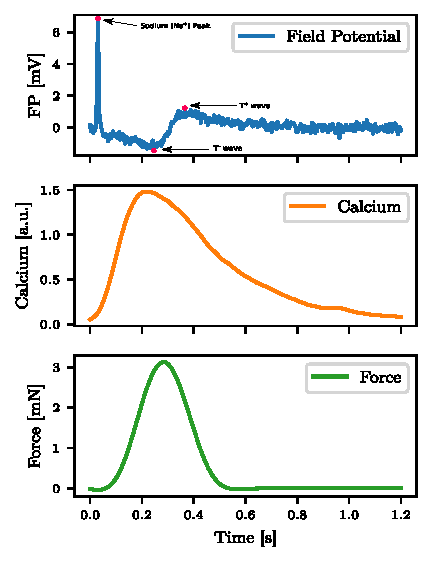
\includegraphics[width=\textwidth]{plots/chapter_3/single_contraction_plot_annotatedpdf.pdf}
                    \caption[Non-arrhythmic contraction]{}
                    % \textbf{Single contraction cycle}  \par \small 
                    % Synchronized view of a single contraction cycle across modalities: (a) Field potential (Na$^+$ peak, T$^-$, T$^+$ waves), (b) calcium transient, and (c) force signal.}
                    \label{fig:single-contraction}
                \end{subfigure}
                ~~~
                \begin{subfigure}[b]{0.4\textwidth}
                    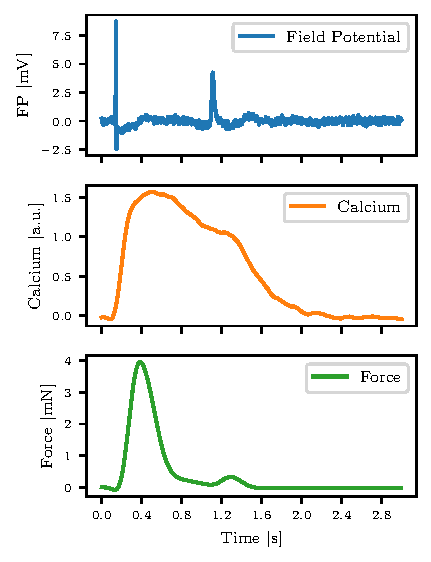
\includegraphics[width=\textwidth]{plots/chapter_3/single_arrythmic_contraction_plot.pdf}
                    \caption[Arrhythmic contraction]{}
                        % \textbf{Arrhythmia morphology} \par \small
                        % Irregular contraction excluded from analysis: 
                        % Multiple force peaks, abnormal calcium decay, 
                        % and disrupted field potential morphology.}
                    \label{fig:arrhythmic-contraction}
                \end{subfigure}
                \caption[Contraction Types]{\textbf{Contraction Types} \textbf{(a) Non-arrhythmic contraction}: Synchronized view of a single contraction event across modalities: (i) Field potential (Na$^+$ peak, T$^-$, T$^+$ waves), (ii) Calcium transient, and (iii) Force signal. \textbf{(b) Arrhythmic Contraction}: Irregular contractions, excluded from analysis, characterized by multiple force peaks, abnormal calcium decay, or disrupted field potential morphology.}
            \end{figure}

            \begin{figure}[h]
                \centering
                \begin{subfigure}[b]{0.3\textwidth}
                    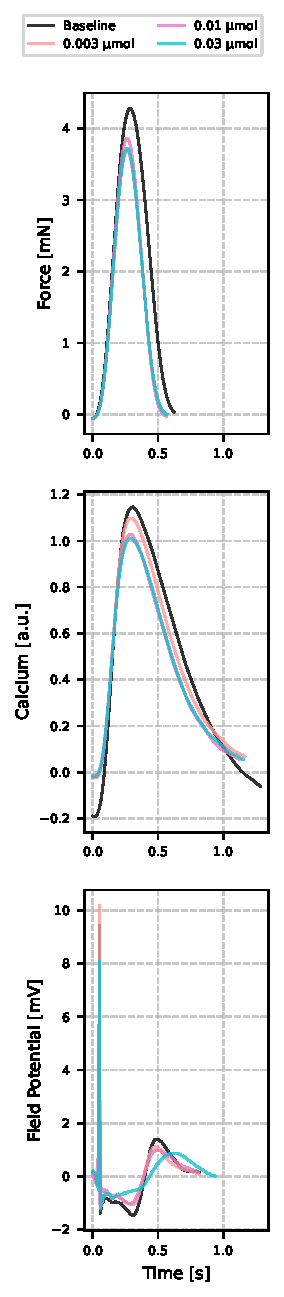
\includegraphics[width=\textwidth, height=0.92\textheight]{plots/chapter_3/average_signals_e4031.pdf}
                    \caption[E-4031 average contraction]{}
                    % \textbf{Single contraction cycle}  \par \small 
                    % Synchronized view of a single contraction cycle across modalities: (a) Field potential (Na$^+$ peak, T$^-$, T$^+$ waves), (b) calcium transient, and (c) force signal.}
                    \label{fig:e4031-average}
                \end{subfigure}
                ~
                \begin{subfigure}[b]{0.3\textwidth}
                    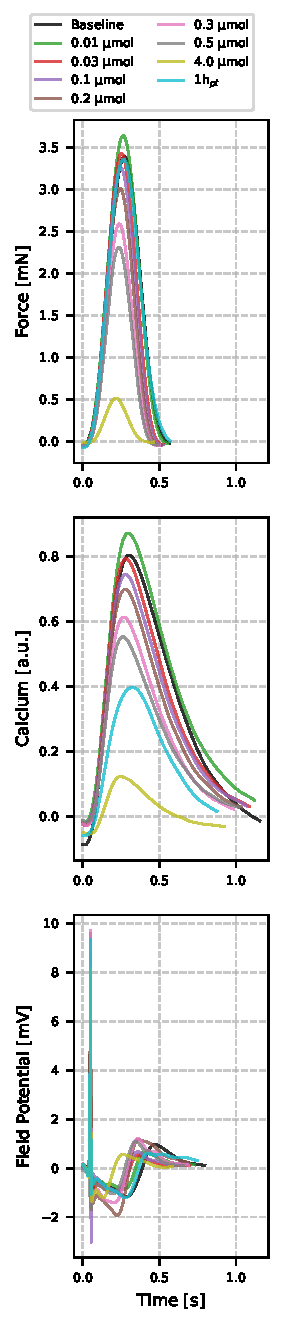
\includegraphics[width=\textwidth, height=0.92\textheight]{plots/chapter_3/average_signals_nifedipine.pdf}
                    \caption[Nifedipine average contraction]{}
                        % \textbf{Arrhythmia morphology} \par \small
                        % Irregular contraction excluded from analysis: 
                        % Multiple force peaks, abnormal calcium decay, 
                        % and disrupted field potential morphology.}
                    \label{fig:nifedipine-average}
                \end{subfigure}
                ~
                \begin{subfigure}[b]{0.34\textwidth}
                    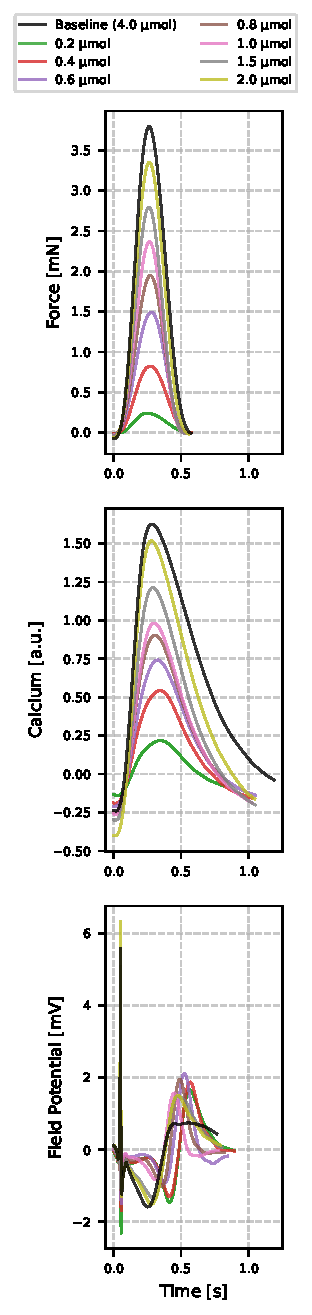
\includegraphics[width=\textwidth, height=0.927\textheight]{plots/chapter_3/average_signals_ca_titration.pdf}
                    \caption[Calcium Titration average contraction]{}
                        % \textbf{Arrhythmia morphology} \par \small
                        % Irregular contraction excluded from analysis: 
                        % Multiple force peaks, abnormal calcium decay, 
                        % and disrupted field potential morphology.}
                    \label{fig:ca-titration-average}
                \end{subfigure}
               \caption[Average Tissue Response in Pharmacological Experiments]{\textbf{Average Tissue Response in Pharmacological Experiments.} \textbf{(a) E-4031}: Averaged contraction signals recorded under baseline conditions and after E-4031 treatment, presented for three modalities (Force, Calcium and Field Potential) along a shared time axis. \textbf{(b) Nifedipine}: Tissue contraction response under baseline and Nifedipine treatment. \textbf{(c) Calcium Titration}: Contraction dynamics observed across different calcium concentrations.}
                \label{fig:average-contraction}
            \end{figure}

          With multimodal data collected under pharmacological perturbations, the next step involves preprocessing to enhance signal fidelity. This includes filtering noise, identifying contraction events, and removing arrhythmias (Figure~\ref{fig:arrhythmic-contraction}). The following chapter details the preprocessing workflow and feature extraction techniques used to derive biologically meaningful insights from the recorded signals.

\chapter{Data Preprocessing and Feature Extraction}
\label{data-prep}
    After acquiring raw multimodal data, a structured preprocessing pipeline was applied to improve signal fidelity and remove systematic noise. Once preprocessed, contraction events were identified using peak detection algorithms, followed by arrhythmia classification to exclude irregular contractions. Finally, biologically relevant features were extracted from each contraction event to facilitate downstream analysis. The peak detection methodology, originally developed in an arrhythmia classification study \cite{Sarwar2024}, was refined in this work, particularly for Field Potential (FP) signal. The following sections detail these preprocessing and feature extraction steps.

   \section{Preprocessing and Signal Enhancement}
   \label{signal-enhancement}
   Each signal in functional MT data i.e Force, Calicum and FP underwent a series of preprocessing steps to improve data quality and eliminate systematic noise.
   \subsection{Force Signal Preprocessing}
   \label{sec:force-prep}

    \begin{enumerate}
        \item \textbf{Systematic Noise Removal}  
        \begin{itemize}
            \item High-frequency noise, primarily originating from external interference, was identified through frequency-domain analysis.
            \item A 5th-order Butterworth low-pass filter was applied, with the cutoff frequency set to eliminate components exceeding the heart's physiological frequency limit (\SI{3.6}{\hertz}) while preserving critical contraction-related components.
        \end{itemize}
    
        \item \textbf{Baseline Offset Correction}  
        \begin{itemize}
            \item The force signal often contains an inherent baseline shift due to sensor drift or passive tissue tension.
            \item A histogram-based approach is used, where a Gaussian curve is fitted to the histogram peak for approximating the noise density.
            \item The mean of the fitted Gaussian is taken as the offset value and subtracted from the entire signal, ensuring accurate force measurements (Figure \ref{fig:force-histogram}).
        \end{itemize}
    
        \item \textbf{Smoothing and Noise Reduction}  
        \begin{itemize}
            \item A Savitzky-Golay (SavGol) \cite{SavitzkyGolayWiki} filter is applied to the baseline-corrected signal for smoothing while preserving peaks and critical features associated with cardiomyocyte contractions.
        \end{itemize}
    \end{enumerate}
    
    The final preprocessed force signal is \textbf{filtered, baseline-corrected, and smoothed} (Figure~\ref{fig:force-preprocessed}), providing a robust representation of contractile behavior. For a more detailed discussion of the methodology, refer to \cite[Section 3.1]{Sarwar2024}.  

    % \begin{figure}[H]
    %         \centering
    %         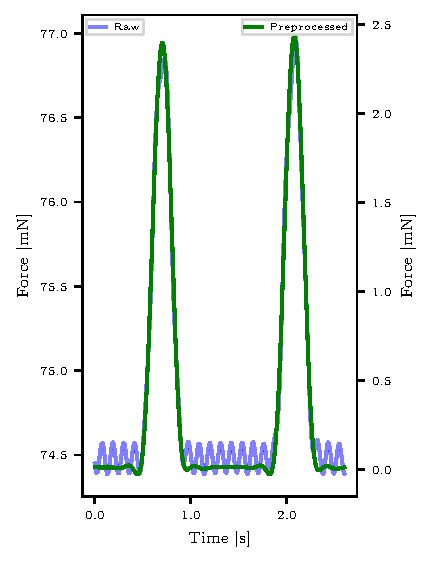
\includegraphics[]{plots/chapter_3/force_raw_vs_preprocessed.pdf}
    %         \caption[Force signal enhancement]{
    %             \textbf{Force signal enhancement} \par \small
    %             Raw force (Blue, Axis: Left), Preprocessed force (Green, Axis: Right).
    %             Preprocessing steps: (1) Systematic noise removal, (2) Baseline correction, 
    %             and (3) Savitzky-Golay filtering.}
    %         \label{fig:force-preprocessed}
    % \end{figure}

     \begin{figure}[H]
                \centering

                 \begin{subfigure}[b]{0.45\textwidth}
                    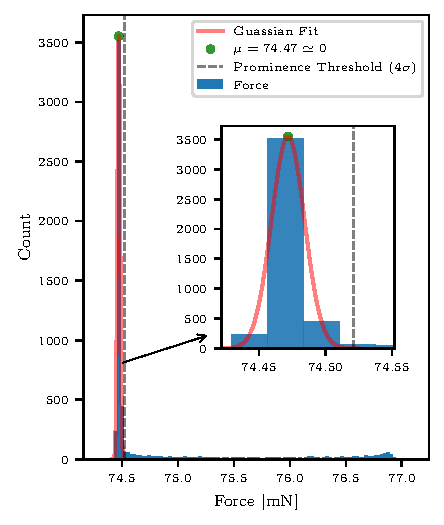
\includegraphics[width=\textwidth, height=0.49\textheight]{plots/chapter_3/force_histogram_inset.pdf}
                    \caption[Force Histogram]{}
                        % \textbf{Arrhythmia morphology} \par \small
                        % Irregular contraction excluded from analysis: 
                        % Multiple force peaks, abnormal calcium decay, 
                        % and disrupted field potential morphology.}
                    \label{fig:force-histogram}
                \end{subfigure}
                ~
                \begin{subfigure}[b]{0.45\textwidth}
                   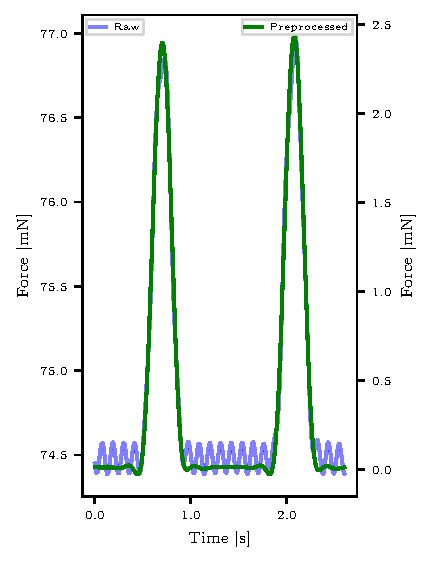
\includegraphics[]{plots/chapter_3/force_raw_vs_preprocessed.pdf}
                    \caption[Force signal enhancement]{}
                        % \textbf{Force signal enhancement} \par \small
                        % Raw force (Blue, Axis: Left), Preprocessed force (Green, Axis: Right).
                        % Preprocessing steps: (1) Systematic noise removal, (2) Baseline correction, 
                        % and (3) Savitzky-Golay filtering.}
                    \label{fig:force-preprocessed}
                \end{subfigure}
                \caption[Force Preprocessing]{\textbf{Force Preprocessing.} \textbf{(a)} Histogram of the force signal with a fitted Gaussian curve centered at the histogram peak. The Gaussian mean, representing the baseline offset, is subtracted from the signal during baseline correction to achieve a zero-mean baseline. A 4$\sigma$ threshold from this fit is then used as the prominence threshold for peak detection (see Section \ref{force-peak-detection}). \textbf{(b)} Comparison of the raw force signal (blue) and its preprocessed version (green), demonstrating the combined effects of noise removal, baseline correction, and smoothing on enhancing the signal quality.}

    \end{figure}

    \newpage
    \subsection{Calcium Signal Preprocessing}
    \label{sec:calc-prep}

    \begin{enumerate}
        \item \textbf{Baseline Offset Correction}  
        \begin{itemize}
            \item The calcium signal exhibited a sloped baseline or pedestal offset, requiring correction to ensure accurate intracellular calcium measurements.
            \item A \textit{two-step correction process} is applied:
            \begin{itemize}
                \item First, a method similar to force signal correction is used, where a Gaussian curve is fitted around the peak corresponding to baseline noise in the histogram. The mean of the fitted Gaussian serves as the initial estimated baseline.
                \item To refine this estimation, a Random Sample Consensus (RANSAC) algorithm is applied. RANSAC fits a regression line to data points around the initial estimated baseline by utilizing the standard deviation of the fitted guassian, ensuring a more robust correction (Figure \ref{fig:calc-ransac}).
            \end{itemize}
            \item The refined baseline estimate is then subtracted from the entire calcium signal to achieve accurate baseline correction.
        \end{itemize}
    
        \item \textbf{Smoothing}  
        \begin{itemize}
            \item A Savitzky-Golay (SavGol) filter is applied to the baseline-corrected signal for further smoothing of the signal which enhances the signal-to-noise ratio.
        \end{itemize}
    
        \item \textbf{Time-Axis Correction}  
        \begin{itemize}
            \item A time-axis adjustment is performed to correct for a hardware-induced delay affecting calcium signal recordings.
            \item This step ensures accurate synchronization with other signals, allowing for more precise multimodal analysis.
        \end{itemize}
    \end{enumerate}
    
    The final preprocessed calcium signal is \textbf{baseline-corrected, smoothed, and time-adjusted} (Figure~\ref{fig:calc-preprocessed}). A more detailed explanation of these preprocessing methods can be found in \cite[Section 3.3]{Sarwar2024}.  

    % \begin{figure}[H]
    %         \centering
    %         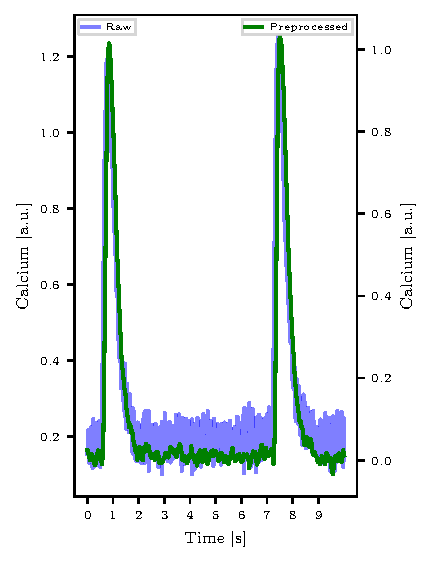
\includegraphics[]{plots/chapter_3/calc_raw_vs_preprocessed.pdf}
    %         \caption[Calcium signal adjustments]{
    %             \textbf{Calcium signal adjustments} \par \small
    %             Raw calcium (Blue, Axis: Left), Preprocessed calcium (Green, Axis: Right).
    %             Preprocessing workflow: (1) Time correction for hardware delay, (2) Baseline correction, 
    %             and (3) Savitzky-Golay filtering.}
    %         \label{fig:calc-preprocessed}
    %     \end{figure}

    \begin{figure}[t]
                \centering
                 \begin{subfigure}[b]{0.4\textwidth}
                    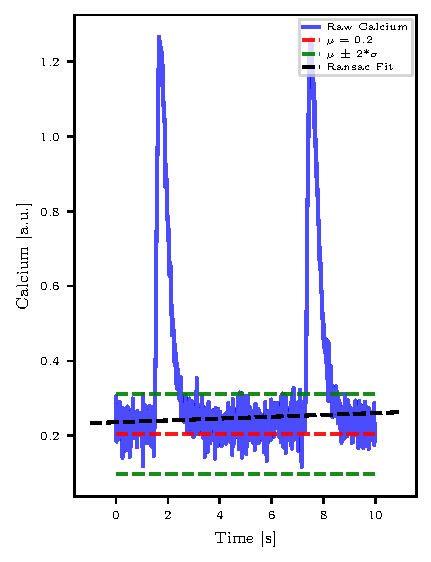
\includegraphics[width=\textwidth, keepaspectratio]{plots/chapter_3/calc_ransac_fit.pdf}
                    \caption[Calcium Ransac Fit]{}
                        % \textbf{Arrhythmia morphology} \par \small
                        % Irregular contraction excluded from analysis: 
                        % Multiple force peaks, abnormal calcium decay, 
                        % and disrupted field potential morphology.}
                    \label{fig:calc-ransac}
                \end{subfigure}
                ~
                \begin{subfigure}[b]{0.4\textwidth}
                   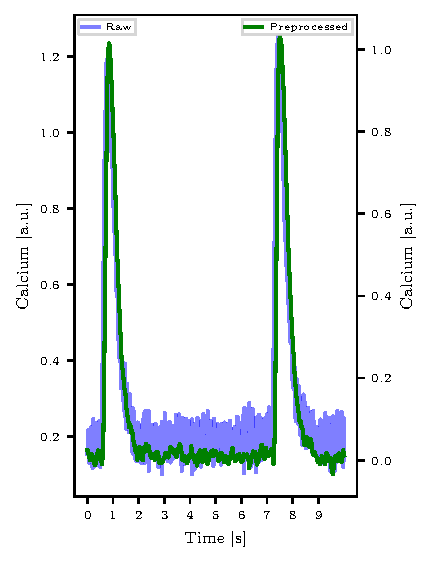
\includegraphics[width=\textwidth, keepaspectratio]{plots/chapter_3/calc_raw_vs_preprocessed.pdf}
                    \caption[Calcium signal enhancement]{}
                        % \textbf{Force signal enhancement} \par \small
                        % Raw force (Blue, Axis: Left), Preprocessed force (Green, Axis: Right).
                        % Preprocessing steps: (1) Systematic noise removal, (2) Baseline correction, 
                        % and (3) Savitzky-Golay filtering.}
                    \label{fig:calc-preprocessed}
                \end{subfigure}
                \caption[Calcium Preprocessing]{\textbf{Calcium Preprocessing} \textbf{(a)} A 10-second segment of the calcium signal with vertical lines indicating the mean (red) and $\pm 2 $ standard deviations ($\sigma$, green) of the fitted gaussian distribution around signal's histogram maximum. A RANSAC linear fit (black) is applied to the data points within a region of $\mu \pm 2 \sigma$ to estimate baseline slope and use it as subtraction offset for baseline correction. \textbf{(b)} Comparison of the raw calcium signal with its preprocessed version.}
    \end{figure}
    

    \subsection{Field Potential Signal Preprocessing}

    The preprocessing of Field Potential (FP) signal was performed in two stages. The initial preprocessing, conducted as part of prior work \cite{Sarwar2024}, focused on identifying high-quality signal channels and applying basic denoising techniques. This involved classifying channels based on signal quality, averaging selected channels to enhance stability, and applying a low-pass filter for noise reduction. Although initial preprocessing enhanced signal clarity, residual high-frequency noise and channel variability still affected the data. To address this, advanced denoising techniques, including Discrete Wavelet Transform (DWT) decomposition, were applied in this thesis to further refine signal quality and improve robustness in downstream analysis.
    
    \subsubsection{Channel Quality Classification and Averaging}
    \label{channel-quality-classification}
    
    \begin{itemize}
        \item \textbf{Channel Quality Classification}  
        \begin{itemize}
            \item As stated in Section \ref{sec:daq}, FP recordings consisted of signals from 32 MEA channels, each exhibiting varying signal quality.
            \item The channels from a random subset of FP recordings were selected and manually labeled into three categories: \textbf{bad, medium} and \textbf{good}, based on their signal characteristics (Figure \ref{fig:mea-channel-categories}).
            \item Statistical features such as \textit{mean, median, mode, standard deviation}, and various other time and frequency domain descriptors were extracted from each channel using the \textbf{Time Series Feature Extraction Library (TSFEL)} \cite{barandas2020tsfel}.
            \item A Random Forest classifier with `balanced' class weights (due to high class imbalance) was trained on these extracted features to learn the mapping between statistical features and channel quality.
            \item The trained model achieved a high classification accuracy, effectively distinguishing high-quality channels for further analysis.
        \end{itemize}
    
        \item \textbf{Selection and Averaging of Good Channels}  
        \begin{itemize}
            \item Only channels classified as "good" were retained for further analysis.
            \item The signals from all good channels were averaged to obtain a single representative FP signal.
            % \item This averaging approach helped improve timing consistency and reduce variability.
        \end{itemize}
    
        \item \textbf{Initial Noise Filtering}  
        \begin{itemize}
            \item A low-pass filter was applied to the averaged signal, preserving key features of the FP signal while attenuating high-frequency noise.
        \end{itemize}
    \end{itemize}
    
    For a more detailed explanation of these preprocessing steps, refer to \textit{Section 3.4} of previous work \cite{Sarwar2024}. An averaged FP signal is shown in Figure \ref{fig:mea-final}

    % \begin{figure}[H]
    %         \centering
    %         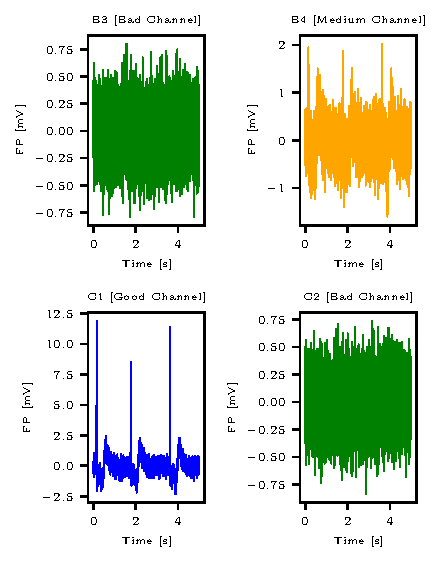
\includegraphics[width=0.8\textwidth, keepaspectratio]{plots/chapter_3/mea_4_channels_plot.pdf}
    %         \caption[MEA channel quality classification]{
    %            \textbf{MEA channel quality classification} \par \small
    %             Channel categorization: 
    %             (A) Good quality (Blue, capturing all aspects of FP signal), 
    %             (B) Medium-quality (Orange, capturing Na$^+$ peaks only), 
    %             (C) Bad-quality (Green, complete noise).}
    %         \label{fig:mea-channel-categories}
    %     \end{figure}
    
    %     \begin{figure}[H]
    %         \centering
    %         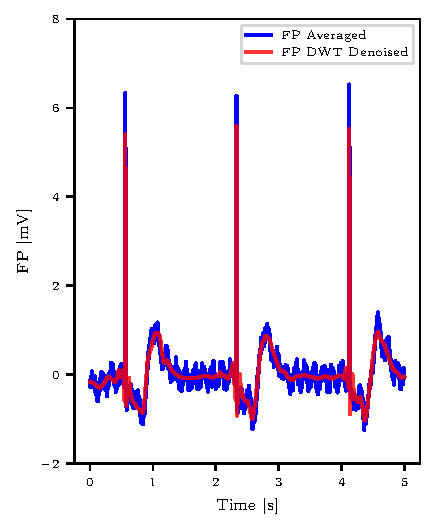
\includegraphics[width=1\textwidth, keepaspectratio]{plots/chapter_3/mea_avg_filtered_preprocessed_plot.pdf}
    %         \caption[Processed field potential]{
    %         \textbf{Processed field potential} \par \small
    %         Averaged FP signal from high-quality MEA channels 
    %         after low-pass filtering. }
    %         \label{fig:mea-final}
    %     \end{figure}    



    \begin{figure}[H]
                \centering
                 \begin{subfigure}[b]{0.45\textwidth}
                    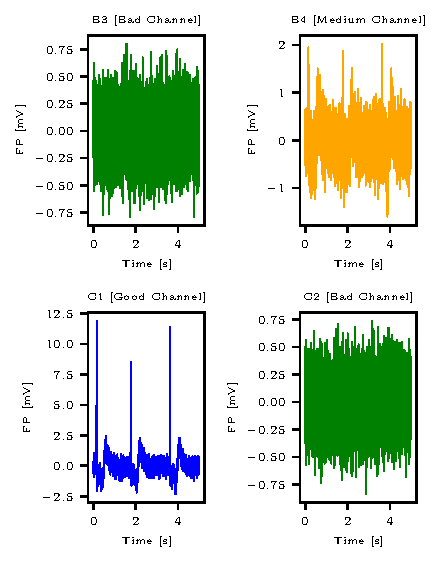
\includegraphics[width=\textwidth,keepaspectratio]{plots/chapter_3/mea_4_channels_plot.pdf}
                    \caption[MEA channel quality classification]{}
                        % \textbf{Arrhythmia morphology} \par \small
                        % Irregular contraction excluded from analysis: 
                        % Multiple force peaks, abnormal calcium decay, 
                        % and disrupted field potential morphology.}
                    \label{fig:mea-channel-categories}
                \end{subfigure}
                ~
                \begin{subfigure}[b]{0.45\textwidth}
                   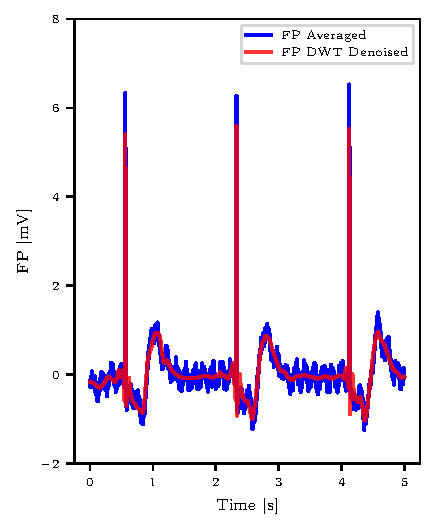
\includegraphics[width=\textwidth, keepaspectratio]{plots/chapter_3/mea_avg_filtered_preprocessed_plot.pdf}
                    \caption[Processed field potential]{}
                        % \textbf{Force signal enhancement} \par \small
                        % Raw force (Blue, Axis: Left), Preprocessed force (Green, Axis: Right).
                        % Preprocessing steps: (1) Systematic noise removal, (2) Baseline correction, 
                        % and (3) Savitzky-Golay filtering.}
                    \label{fig:mea-final}
                \end{subfigure}
                \caption[Field Potential Signal Processing]{\textbf{Field Potential (FP) Signal Processing.} \textbf{(a)} \textbf{MEA Channel Quality Classification}: Channels are categorized as (i) Good (blue), capturing all aspects of the FP signal; (ii) Medium (orange), capturing peaks despite higher noise levels; and (iii) Bad (green), dominated by noise. \textbf{(b)} \textbf{Processed FP}: Comparison of the averaged and low-pass filtered FP signal (blue) from high-quality channels with its DWT-denoised version (red), illustrating the improvement in signal clarity.}
    \end{figure}
    
    \subsubsection{DWT-Based Denoising}
    
        In this thesis, further FP signal denoising was performed to enhance signal quality. Despite the initial noise reduction, high-frequency noise was still present, as seen in Figure~\ref{fig:mea-final}. To address this, Discrete Wavelet Transform (DWT) \cite{DWTWiki} was applied to decompose the signal into different frequency components and selectively remove noise.
    
            The frequency composition of the FP was first analyzed using the Fourier Transform (Figure~\ref{fig:fp_fft}), which revealed the dominant signal energy components within the \textbf{0-200 \SI{}{\textbf{\hertz}} range}, as components outside this range were attenuated through the low-pass filter (Section \ref{channel-quality-classification}). This information guided the denoising approach by selectively modifying the wavelet coefficients corresponding to high-to-medium frequency components.
            
            DWT decomposition was performed using the \textbf{Daubechies-4 (`db4') wavelet} with whole-sample symmetric padding (implemented as `reflect' in PyWavelets \cite{Lee2019}). This decomposition method separates the signal into \textbf{approximation coefficients} \textbf{(\(\bm{A_n}\))}, which capture low-frequency trends, and \textbf{detail coefficients} \textbf{(\(\bm{D_n}\))}, which represent high-frequency variations. Each level of decomposition halves the frequency range of the previous level, with the first level spanning 500-1000 \SI{}{\hertz}, the second level covering 250-500 Hz, and so on. At each step, only the detail coefficients (\(\bm{D_n}\)) are further decomposed, while the approximation coefficients remain unchanged. The decomposition continued up to \textbf{14 levels}, starting from the \textbf{Nyquist frequency (}\(\bm{F_s/2 = 1000}\) \SI{}{\textbf{\hertz}}) where $F_s$ is the sampling rate of FP signal. 
            
            \begin{table}[H]
                \centering
                \caption{Decomposition and Transformation of Averaged FP Signal using DWT}
                \label{tab:fp_dwt_decomposition}
                \begin{tabular}{c c c}
                    \toprule
                    \textbf{Level} & \textbf{Frequency Range (Hz)} & \textbf{Transformation Applied} \\
                    \midrule
                    1 & 500 - 1000  & Detail Coefficients Removed (\(D_1 = 0\)) \\
                    2 & 250 - 500   & Detail Coefficients Removed (\(D_2 = 0\)) \\
                    3 & 125 - 250   & Soft Thresholding (\(\lambda = 0.5\)) \\
                    4 & 62.5 - 125  & Soft Thresholding (\(\lambda = 0.5\)) \\
                    5 & 31.25 - 62.5 & Soft Thresholding (\(\lambda = 0.5\)) \\
                    6 & 15.62 - 31.25 & Soft Thresholding (\(\lambda = 0.5\)) \\
                    7 & 7.81 - 15.62 & Soft Thresholding (\(\lambda = 2.5\)) \\
                    8 & 3.90 - 7.81 & Soft Thresholding (\(\lambda = 2.5\)) \\
                    9 - 14 & \( < 3.9 \) & No Transformation Applied \\
                    \bottomrule
                \end{tabular}
            \end{table}
            
            Denoising was performed by modifying the detail coefficients while preserving the essential signal structure. The high-frequency detail coefficients at levels 1 and 2 were completely removed (\(\bm{D_1, D_2 = 0}\)), eliminating components above \SI{250}{\hertz}. Soft thresholding was applied to the detail coefficients of levels 3 to 8. A threshold of \(\bm{\lambda = 0.5}\) for levels 3 to 6 and a higher threshold of \(\bm{\lambda = 2.5}\) for levels 7 and 8 to suppress low-frequency fluctuations.  These threshold values were selected based on empirical evaluation, testing different values and choosing those that visibly demonstrated optimal noise suppression while preserving signal integrity. Levels 9 to 14, corresponding to frequencies below  \SI{3.9}{\hertz}, were retained as they contribute to slow moving trends. 
            
            Soft thresholding was applied using the following transformation:
            
            \[
            D'_n(x, \lambda)  = 
            \begin{cases} 
            \text{sign}(x) \cdot (\lvert x \rvert - \lambda) & \text{if } \lvert x \rvert > \lambda \\
            0 & \text{otherwise}
            \end{cases}
            \]
            
            where \( x \) represents the wavelet coefficients, and \( \lambda \) is the threshold value. This function reduces small fluctuations while preserving larger signal components, effectively suppressing noise without distorting the true signal. The frequency breakdown and transformations applied at each level are summarized in Table~\ref{tab:fp_dwt_decomposition}.  Figure \ref{fig:fp_dwt} shows exemplary levels to illustrate the effect of thresholding transformations on detail coefficients.
            
            After modifying the wavelet coefficients, the Inverse Discrete Wavelet Transform (IDWT) was applied to reconstruct the denoised signal. The comparison of the original (averaged FP) and DWT denoised signal is presented in Figure \ref{fig:mea-final}, demonstrating the removal of high-frequency noise and the preservation of the essential FP signal features. 
            
            Additionally, the Fourier Transform of the original and denoised signals (Figure~\ref{fig:fp_fft}) confirms the suppression of noise components, validating the effectiveness of the denoising process. The preprocessed FP signal obtained after denoising was used for subsequent analysis.

            % \begin{figure}[H]
            %     \centering
            %     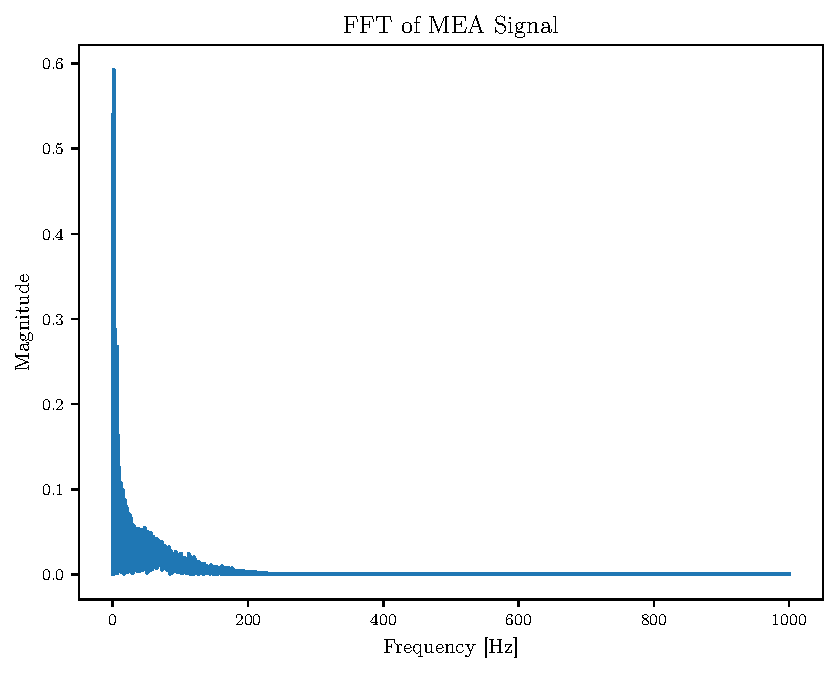
\includegraphics[width=1\textwidth, keepaspectratio]{plots/chapter_3/mea_sft_fft.pdf}
            %     \caption[Field Potential Frequency analysis]{
            %     \textbf{Field Potential Frequency analysis} \par \small
            %     Field Potential Fourier transform revealing dominant signal energy 
            %     below 200 \SI{}{\hertz}.}
            %     \label{fig:fp_fft}
            % \end{figure}

            % \begin{figure}[H]
            %     \centering
            %     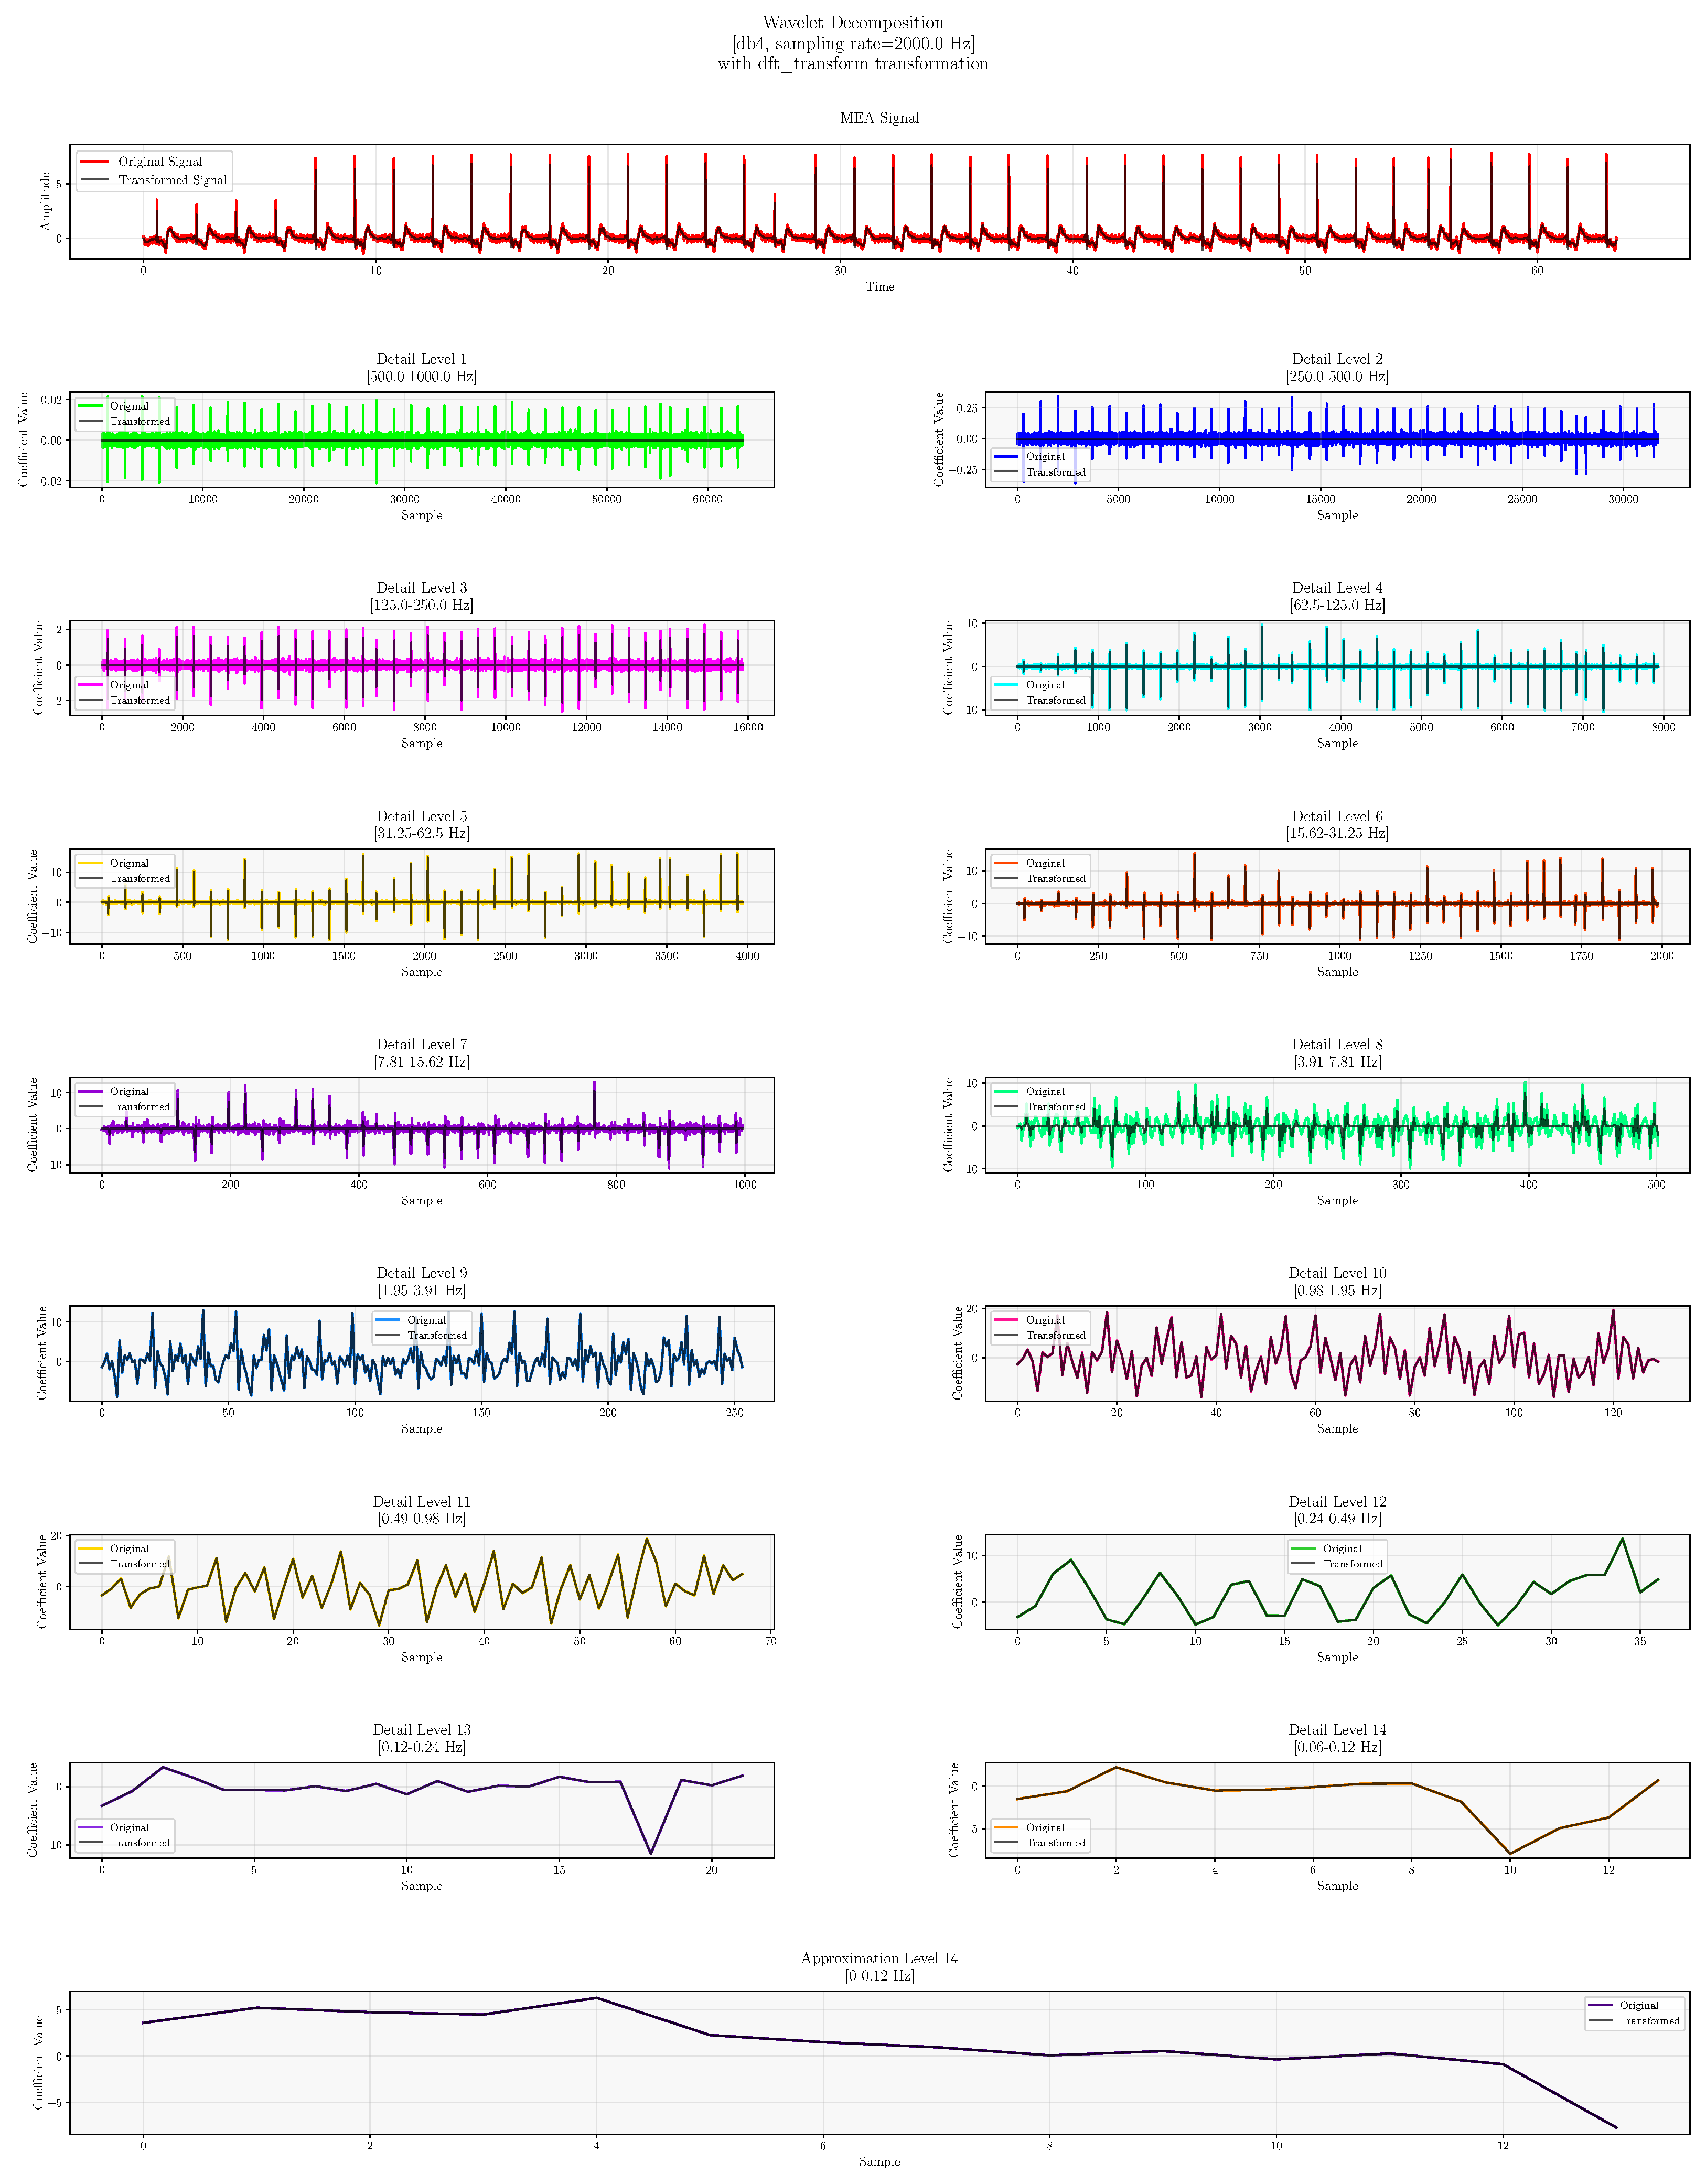
\includegraphics[width=1\textwidth, keepaspectratio]{plots/chapter_3/mea_sft_wavelet_transformed.pdf}
            %     \caption[Field Potential DWT-based denoising strategy]{
            %             \textbf{Field Potential DWT-based denoising strategy}  \par \small
            %             DWT 14-level Daubechies-4 decomposition: 
            %             Levels 1-2 removed (500-1000 \SI{}{\hertz}), 
            %             Levels 3-6 soft-thresholded ($\lambda$=0.5), 
            %             Levels 7-8 soft-thresholded ($\lambda$=2.5), 
            %             Levels 9-14 retained.}
            %     \label{fig:fp_dwt}
            % \end{figure}

            \begin{figure}[H]
                \centering
                 \begin{subfigure}[b]{0.4\textwidth}
                    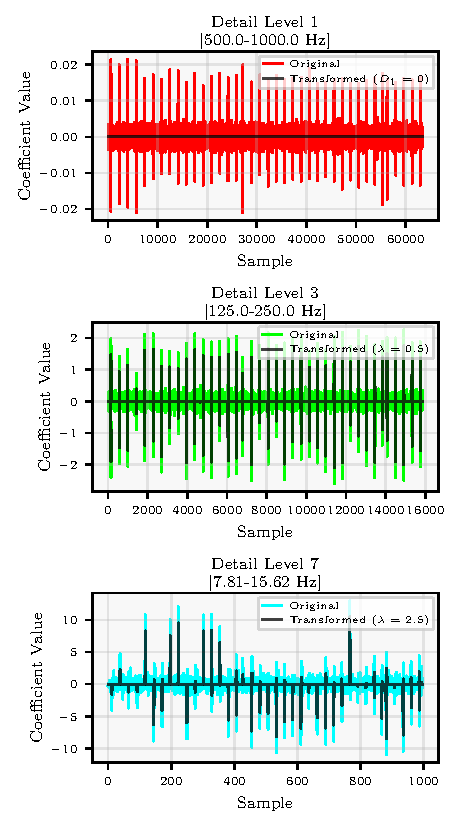
\includegraphics[width=\textwidth, height=0.47\textheight, keepaspectratio]{plots/chapter_3/mea_sft_wavelet_details_selected.pdf}
                    \caption[Field Potential DWT-based denoising strategy]{}
                        % \textbf{Arrhythmia morphology} \par \small
                        % Irregular contraction excluded from analysis: 
                        % Multiple force peaks, abnormal calcium decay, 
                        % and disrupted field potential morphology.}
                    \label{fig:fp_dwt}
                \end{subfigure}
                ~
                \begin{subfigure}[b]{0.45\textwidth}
                   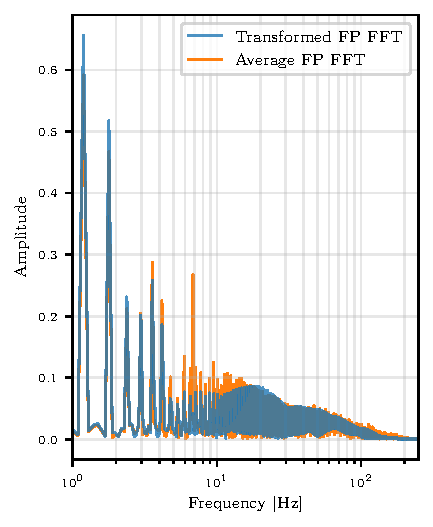
\includegraphics[width=\textwidth,keepaspectratio]{plots/chapter_3/mea_sft_wavelet_comparison_fft.pdf}
                    \caption[Processed field potential]{}
                        % \textbf{Force signal enhancement} \par \small
                        % Raw force (Blue, Axis: Left), Preprocessed force (Green, Axis: Right).
                        % Preprocessing steps: (1) Systematic noise removal, (2) Baseline correction, 
                        % and (3) Savitzky-Golay filtering.}
                    \label{fig:fp_fft}
                \end{subfigure}
                \caption[Field Potential Signal Processing]{\textbf{(a) Effect of DWT-based Denoising on FP Signal}: Detail coefficients of the FP signal at selected decomposition levels: Level 1 (\(D_1\)) shows complete removal of coefficients for high-frequency noise reduction, Level 3 applies soft thresholding with \(\lambda = 0.5\), and Level 7 applies soft thresholding with \(\lambda = 2.5\) to suppress medium-to-low frequency noise. \textbf{(b) FFT of FP signals}: Comparison of the Fourier Transform (FFT) components for the original (averaged FP, orange) and DWT-denoised FP signal (blue) is shown, with the amplitude axis log-transformed to clearly illustrate the attenuation of noise components after denoising.}
             \end{figure}

            
    
    \section{Identification of Contraction Events}
    \label{contraction-events}
     After preprocessing, the next step was precise contraction event detection, which is critical for extracting biologically relevant features. This required accurate peak identification, as each detected peak corresponds to a distinct contraction. A prominence-thresholding-based peak detection logic was adapted from an arrhythmia classification study \cite{Sarwar2024} to detect peaks in force and calcium signals. The high-level overview of the method is described in the following section. For the FP signal, a new method for deriving the prominence threshold was developed.

     \subsection{Force and Calcium Peak Detection}
     A peak’s \textbf{prominence} quantifies its relative importance by measuring the vertical difference between the peak's apex and its lowest contour point. A higher prominence indicates a more distinct peak, making it a robust criterion for peak selection. To implement this, the \texttt{find\_peaks}\cite{SciPyFindPeaks} method from SciPy signal processing module was utilized, with a dynamically determined prominence threshold tailored to each measurement.

    To define an appropriate prominence threshold, the histogram of the preprocessed signal was analyzed. A Gaussian curve was fitted around the peak of the preprocessed signal. Baseline correction (Section \ref{sec:force-prep} \& \ref{sec:calc-prep}) ensures that the dominant noise distribution is centered around zero, i.e $\mu=0$. The standard deviation ($\sigma$) of this fitted Gaussian was utilized for determining prominence threshold, and peaks were retained if their prominence exceeded a threshold set at \textbf{+4 standard deviations}. This thresholding method is based on the statistical principle that approximately 99.9\% of data points in a normal distribution lie within four standard deviations, ensuring that only the most relevant peaks are selected.
    
    This prominence-based approach effectively identifies contraction peaks in both force and calcium signals, ensuring robust detection of contraction events (Figure \ref{fig:force-calc-peaks}). A more detailed explanation of this methodology can be found in \cite[Section 4.1]{Sarwar2024}

    % \begin{figure}[H]
    %             \centering
    %              \begin{subfigure}[b]{0.45\textwidth}
    %                 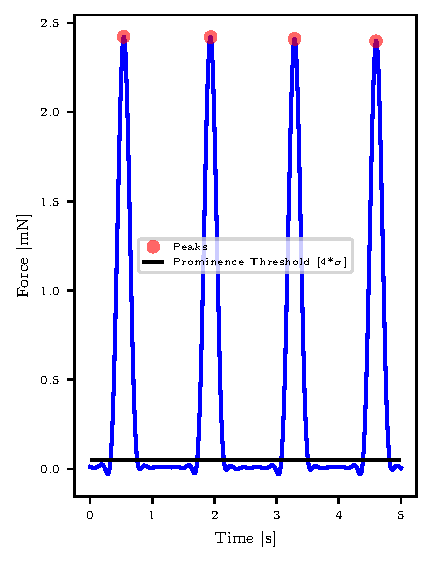
\includegraphics[width=\textwidth, keepaspectratio]{plots/chapter_3/force_peaks_plot.pdf}
    %                 \caption[Force Peaks]{}
    %                     % \textbf{Arrhythmia morphology} \par \small
    %                     % Irregular contraction excluded from analysis: 
    %                     % Multiple force peaks, abnormal calcium decay, 
    %                     % and disrupted field potential morphology.}
    %                 \label{fig:force-peaks}
    %             \end{subfigure}
    %             ~
    %             \begin{subfigure}[b]{0.45\textwidth}
    %                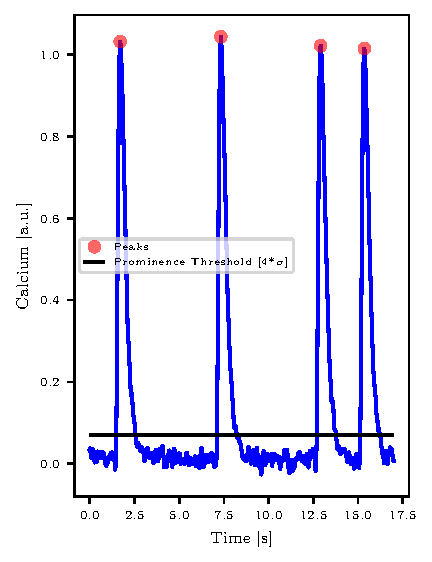
\includegraphics[width=\textwidth,keepaspectratio]{plots/chapter_3/calc_peaks_plot.pdf}
    %                 \caption[Calcium Peaks]{}
    %                     % \textbf{Force signal enhancement} \par \small
    %                     % Raw force (Blue, Axis: Left), Preprocessed force (Green, Axis: Right).
    %                     % Preprocessing steps: (1) Systematic noise removal, (2) Baseline correction, 
    %                     % and (3) Savitzky-Golay filtering.}
    %                 \label{fig:calc-peaks}
    %             \end{subfigure}
    %             \caption[Peak Detection via Prominence Threshold]{\textbf{Peak Detection via Prominence Threshold.} (a) \textbf{Force Signal:} Using SciPy's \texttt{find\_peaks}, force peaks are detected by applying a dynamic prominence threshold set at 4 standard deviations ($\sigma$) of the noise distribution, ensuring that only significant contraction events are identified. (b) \textbf{Calcium Signal:} The same method is used to detect calcium peaks, capturing the most relevant contraction events while filtering out noise.}
    % \end{figure}

    \begin{figure}[H]
        \centering

        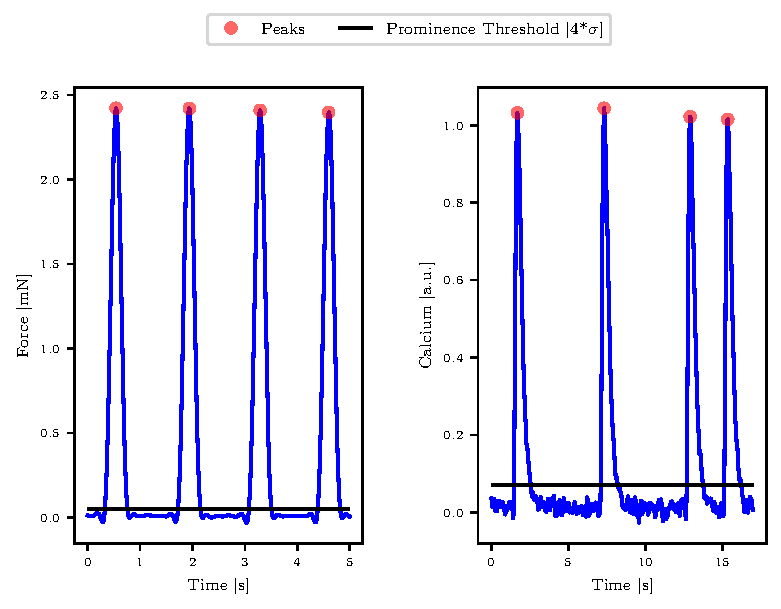
\includegraphics[width=\textwidth, height=0.5\textheight, keepaspectratio]{plots/chapter_3/combined_peaks_plot.pdf}
        \caption[Peak Detection via Prominence Threshold for Force and Calcium signals]{\textbf{Peak Detection via Prominence Threshold for Force and Calcium signals}: Using SciPy's \texttt{find\_peaks}, force and calcium peaks are detected by applying a dynamic prominence threshold set at 4 standard deviations ($\sigma$) of the noise distribution, ensuring that only significant contraction events are identified. }
                        % \textbf{Arrhythmia morphology} \par \small
                        % Irregular contraction excluded from analysis: 
                        % Multiple force peaks, abnormal calcium decay, 
                        % and disrupted field potential morphology.}
        \label{fig:force-calc-peaks}
    \end{figure}

     \subsection{Field Potential Peak Detection}
            
            To detect FP peaks, a Gaussian Mixture Model (GMM) \cite{scikit-learn_gaussian_mixture} was fitted to the signal amplitude distribution. As shown in Figure~\ref{fig:single-contraction}, a single contraction in the FP signal is characterized by a sharp \textbf{sodium} (\(\textbf{Na}^+\)) peak, followed by two \textbf{T-waves}, where the negative component (\(\textbf{T}^-\)) appears before the positive component (\(\textbf{T}^+\)).
            
            The histogram of FP signal  (Figure~\ref{fig:fp-gmm-prominenence-algos}) exhibits three distinct regions:
            \begin{itemize}
                \item A sharp density peak around zero, indicative of baseline noise.
                \item A moderate-density negative peak, corresponding to the \(\text{T}^-\) wave.
                \item A lower-density positive peak, corresponding to the \(\text{T}^+\) wave.
            \end{itemize}

            
            The remaining distribution represents the density of the high-amplitude sodium (\(\text{Na}^+\)) peak.
            
            To model this distribution, a GMM with four components was fitted to the signal. This optimal number of components was selected using the Elbow criterion \cite{thorndike1953hierarchical} applied to the Akaike Information Criterion (AIC) \cite{Akaike_information_criterion} score (Figure~\ref{fig:fp-aic-optimal-gmm}). The fitted GMM parameters (mean \(\bm{\mu}\) and standard deviation \(\bm{\sigma}\)) were then used to derive prominence thresholds for peak detection.
            
            Two different prominence thresholding methods were evaluated:
            
            \begin{enumerate}
                \item \textbf{Algorithm 1:} The Gaussian component with the highest mean (\(\bm{\mu_{\text{hmean}}}\)) was selected, and the prominence threshold was set as:
                \[
                \text{threshold} = \bm{\mu_{\text{hmean}}} + 0.8 \cdot \bm{\sigma_{\text{hmean}}}.
                \]
            
                \item \textbf{Algorithm 2:} The sharpest Gaussian component (i.e., the one with the lowest standard deviation \(\bm{\sigma_{\text{sharp}}}\)) was chosen, with the threshold defined as:
                \[
                \text{threshold} = \bm{\mu_{\text{sharp}}} + 7.5 \cdot \bm{\sigma_{\text{sharp}}}.
                \]
            \end{enumerate}

            % \begin{figure}[h]
            %     \centering
            %     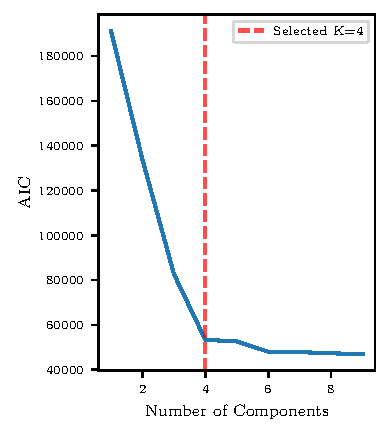
\includegraphics[width=0.6\textwidth, keepaspectratio]{plots/chapter_3/mea_denoised_aic.pdf}
            %     \caption[GMM optimal AIC with Knee]{
            %         \textbf{GMM optimal AIC with Knee}  \par \small
            %         AIC for finding out Optimal GMM components of Denoised Field Potential Signal using Knee criterion [K=4 Optimal].}
            %     \label{fig:fp-aic-optimal-gmm}
            % \end{figure}
            
            % \begin{figure}[h]
            %     \centering
            %     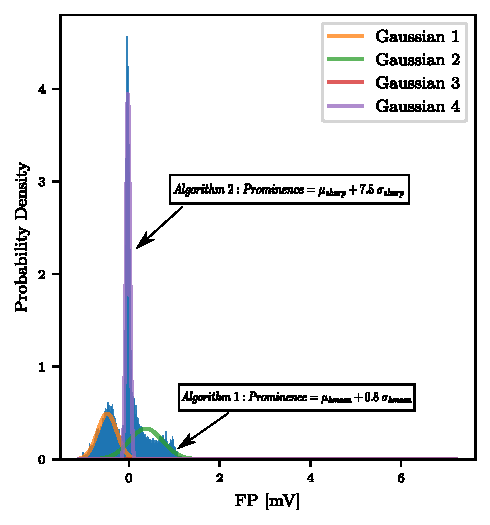
\includegraphics[]{plots/chapter_3/mea_denoised_gmm_components_annotaed_2.pdf}
            %     \caption[GMM-based prominence threshold determination]{
            %        \textbf{GMM-based prominence threshold determination}: Gaussian Mixture Model (K=4) fit to denoised FP: Algorithm 1 threshold (green density): $\mu$\textsubscript{hmean}+~0.8~$\sigma$\textsubscript{hmean}. Algorithm 2 threshold (purple density): $\mu$\textsubscript{sharp}+~7.5~$\sigma$\textsubscript{sharp}.}
            %     \label{fig:fp-gmm-prominenence-algos}
            % \end{figure}

            \begin{figure}[h]
                \centering
                 \begin{subfigure}[b]{0.45\textwidth}
                    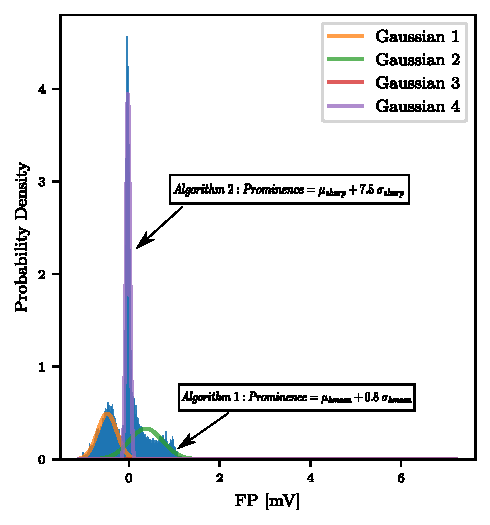
\includegraphics[width=\textwidth,keepaspectratio]{plots/chapter_3/mea_denoised_gmm_components_annotaed_2.pdf}
                    \caption[GMM-based prominence threshold determination]{}
                        % \textbf{Arrhythmia morphology} \par \small
                        % Irregular contraction excluded from analysis: 
                        % Multiple force peaks, abnormal calcium decay, 
                        % and disrupted field potential morphology.}
                   \label{fig:fp-gmm-prominenence-algos}
                \end{subfigure}
                ~
                \begin{subfigure}[b]{0.45\textwidth}
                   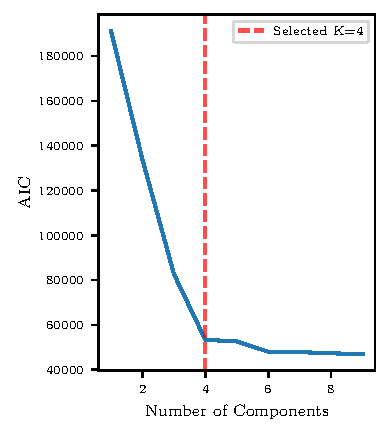
\includegraphics[width=\textwidth,height=0.38\textheight, keepaspectratio]{plots/chapter_3/mea_denoised_aic.pdf}
                    \caption[GMM optimal AIC with Knee]{}
                        % \textbf{Force signal enhancement} \par \small
                        % Raw force (Blue, Axis: Left), Preprocessed force (Green, Axis: Right).
                        % Preprocessing steps: (1) Systematic noise removal, (2) Baseline correction, 
                        % and (3) Savitzky-Golay filtering.}
                    \label{fig:fp-aic-optimal-gmm}
                \end{subfigure}
                \caption[Field Potential Peaks Detection Algorithms Based on GMM]{\textbf{Field Potential Peaks Detection Algorithms Based on GMM.} \textbf{(a) GMM-based Prominence Threshold Determination:} A Gaussian Mixture Model (K=4) is fitted to the denoised FP signal to model its amplitude distribution. Two thresholding methods are evaluated: Algorithm 1 sets the prominence threshold as $\mu_{\text{hmean}}+0.8\,\sigma_{\text{hmean}}$ (green density), while Algorithm 2 uses the sharpest Gaussian component with a threshold of $\mu_{\text{sharp}}+7.5\,\sigma_{\text{sharp}}$ (purple density). \textbf{(b) Optimal GMM Component Selection:} The optimal number of GMM components is determined using the AIC Knee criterion, which identifies K=4 as optimal for the FP signal.}

             \end{figure}
            
            
            Following peak detection, a post-processing step was applied to filter out multiple peaks occurring within a 0.05s window of each peak, retaining the absolute maximum signal value as the peak for that window. After filtering, each peak was categorized as Sodium (\(\text{Na}^+\)), \(\text{T}^-\), or \(\text{T}^+\) based on its half-width at half-maximum (HWHM) and amplitude.
            
            Peak classification was performed based on the following criteria:
           \begin{equation}
            L(P) =
            \begin{cases} 
                \text{Na}^+, & \text{if HWHM}(P) < \text{\SI{0.01}{\s}}, \\
                \text{T}^-, & \text{else if Amplitude}(P) < 0, \\
                \text{T}^+, & \text{otherwise},
            \end{cases}
            \label{eq:peak-classification}
            \end{equation}
            where \textbf{HWHM} represents the peak width at half its maximum height. Sodium (\(\text{Na}^+\)) peaks are sharp with \(\textbf{HWHM < 0.01 \SI{}{\textbf{\s}}}\) (Figure~\ref{fig:fp-na-peak-width}), while \(\text{T}^-\) and \(\text{T}^+\) peaks are differentiated by their negative or positive amplitude. The complete peak detection and classification process is summarized in Procedure~\ref{alg:peak-detection}.

            \begin{figure}[H]
                \centering
                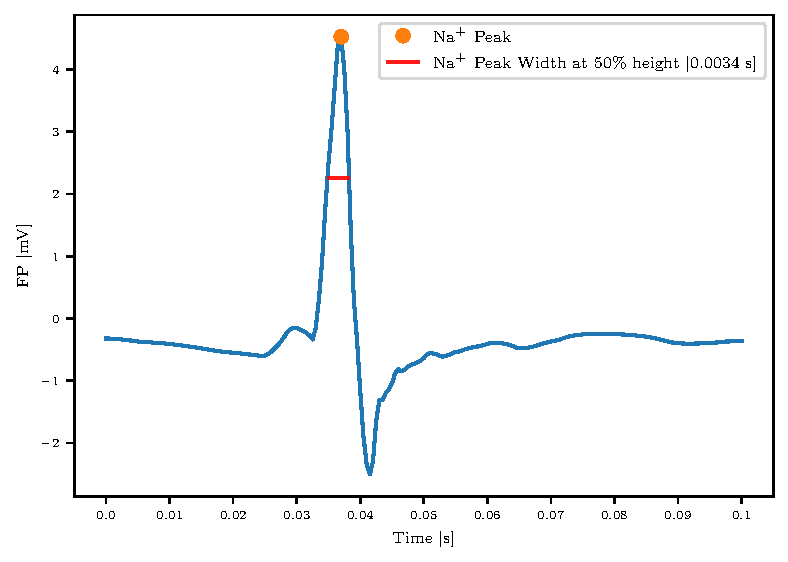
\includegraphics[width=0.6\textwidth, keepaspectratio]{plots/chapter_3/single-na-width-target-case.pdf}
                \caption[Na${^+}$ Peak Decision Factor]{\textbf{Na${^+}$ Peak Decision Factor.} The plot illustrates the criterion used for identifying Na${^+}$ peaks in the FP signal. In this plot, Na${^+}$ peak (shown in orange) is characterized by a half-width at half-maximum (HWHM) of less than 0.01 seconds (marked in red). This threshold serves as a decisive factor for distinguishing sharp Na${^+}$ peaks.}

                \label{fig:fp-na-peak-width}
            \end{figure}
            
            \begin{algorithm}[H]
            \caption{Field Potential Peak Detection}
            \label{alg:peak-detection}
            \textbf{Input:} FP signal, method \(\in\) \{'Algorithm1', 'Algorithm2'\} \\
            \textbf{Output:} Categorized peaks (\(\text{Na}^+, T^-, T^+\))
            \begin{algorithmic}[1]
                \State Fit GMM with 4 components to the signal.
                \State Extract Gaussian parameters (\(\bm{\mu}, \bm{\sigma}\)) from the fitted model.
                \If {method == `Algorithm1'}
                    \State \( hmean\_idx = \arg\max(\bm{\mu}) \)
                    \State \( \bm{\mu_{\text{hmean}}}, \bm{\sigma_{\text{hmean}}} = \bm{\mu}[hmean\_idx], \bm{\sigma}[hmean\_idx] \)
                    \State \( \text{threshold} = \bm{\mu_{\text{hmean}}} + 0.8 \cdot \bm{\sigma_{\text{hmean}}} \)
                \ElsIf {method == `Algorithm2'}
                    \State \( sharp\_idx = \arg\min(\bm{\sigma}) \)
                    \State \( \bm{\mu_{\text{sharp}}}, \bm{\sigma_{\text{sharp}}} = \bm{\mu}[sharp\_idx], \bm{\sigma}[sharp\_idx] \)
                    \State \( \text{threshold} = \bm{\mu_{\text{sharp}}} + 7.5 \cdot \bm{\sigma_{\text{sharp}}} \)
                \EndIf
                \State Detect peaks using prominence threshold.
                \State Apply post-processing: filter multiple peaks within 0.05s window.
                \State Categorize peaks using \(L(P)\) (see Equation~\ref{eq:peak-classification}).
            \end{algorithmic}
            \end{algorithm}
            
            To evaluate the two prominence thresholding methods, eight cases were randomly selected from the dataset. Each peak, along with its category, was manually annotated using the TRAINSET annotation tool \cite{trainset}. The detected peaks and their corresponding labels were compared against the manually annotated ground truth.
            
            Matching was performed using linear cost assignment for bipartite matching, where the cost matrix was defined as:
            \[
            \text{cost}[P_i, P_j] =
            \begin{cases} 
                |t_i - t_j| + 1, & \text{if } L_i \neq L_j \text{ and } L_i = \text{Na}^+,\\
                |t_i - t_j| + 0.5, & \text{if } L_i \neq L_j \text{ and } L_i \neq \text{Na}^+.
            \end{cases}
            \]
            where:
            \begin{itemize}
                \item \(i\) belongs to the indices of ground truth peaks,
                \item \(j\) belongs to the indices of algorithm-detected peaks,
                \item \(t_i, t_j\) are the time indices of peaks \(P_i\) and \(P_j\), and
                \item \(L_i, L_j\) are their respective labels.
            \end{itemize}
            
            The Hungarian algorithm \cite{HungarianAlgorithmWiki} was then applied to determine the optimal assignment score of peaks and labels for each Algorithm. The total cost of the optimal assignment over labeled cases was used to evaluate the performance of the two thresholding methods. The results are summarized in Table~\ref{tab:selected_peak_cases}.
            
            According to the results, Algorithm 2, which uses the sharpest Gaussian component as the threshold, outperformed Algorithm 1 by detecting peaks at a lower overall cost. A single case comparison for each method is shown in Figure~\ref{fig:fp-gmm-thresholding-comparision-single-case}. Algorithm 1 in contrast captured a lot of noise peaks. As a result, Algorithm 2 was selected for FP peak detection across the entire dataset.



            \begin{table}[H]
                \centering
                \caption{Linear Cost Assignment Comparison of Field Potential Peak Detection Methods on Ground Truth.}
                \label{tab:selected_peak_cases}
                \renewcommand{\arraystretch}{1.2} % Adjusts row height for better readability
                \begin{tabular}{p{3cm} *{8}{c} c}
                    \toprule
                    \textbf{Algorithm/Case} & \textbf{1} & \textbf{2} & \textbf{3} & \textbf{4} & \textbf{5} & \textbf{6} & \textbf{7} & \textbf{8} & \textbf{Total} \\
                    \midrule
                    GMM--$\mu_{hmean}$ & 94.0 & 104.0 & 68.0 & 60.0 & 61.43 & 36.0 & 44.0 & 30.0 & 497.43 \\
                    GMM--$\mu_{sharp}$ & 94.0 & 104.0 & 68.0 & 60.0 & 42.10 & 36.09 & 45.25 & 30.0 & 479.44 \\
                    \bottomrule
                \end{tabular}
            \end{table}
            

            \begin{figure}[H]
                \centering
                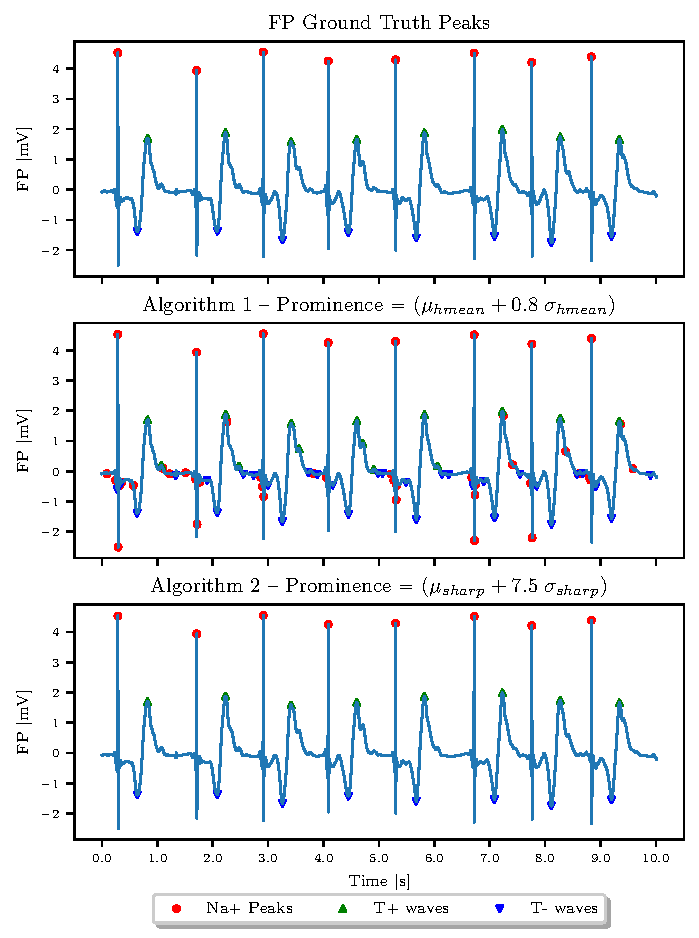
\includegraphics[width=1\textwidth, keepaspectratio]{plots/chapter_3/peak-comparison-target-case.pdf}
                \caption[Field Potential Peak detection comparison]{
                   \textbf{Field Potential Peak Detection Comparison.} The figure presents a side-by-side comparison for a single case: Ground Truth (top), Algorithm 1 (middle), and Algorithm 2 (bottom). Algorithm 2, which uses the sharpest Gaussian component as its threshold, achieves a lower overall cost in peak assignment (see Table~\ref{tab:selected_peak_cases}), whereas Algorithm 1 captures numerous noise peaks. This comparison underlines the superior performance of Algorithm 2 for FP peak detection.
                    }
                \label{fig:fp-gmm-thresholding-comparision-single-case}
            \end{figure}
            
    
   \section{Arrhythmia Detection and Removal}
        \label{sec:arrythmia}
        Arrhythmic contractions are irregular heartbeats that disrupt the normal ECC process. These anomalies require individual analysis and, for this study, they were systematically identified and removed using a machine learning-based arrhythmia classification approach developed during a prior study \cite{Sarwar2024}. The models from that project were integrated into this work to eliminate arrhythmic contractions, ensuring that only non-arrhythmic valid contractions were analyzed. A representative arrhythmic contraction is shown in Figure~\ref{fig:arrhythmic-contraction}, characterized by abnormal signal decay and the presence of multiple peaks.
        
            \subsection{Arrhythmia Classification Framework}
            
            After signal preprocessing and identification of contraction events, the next step was labeling each contraction event. The force signal was selected as the primary reference for arrhythmia labeling due to its higher signal-to-noise ratio (SNR) and consistent peak morphology, making it more reliable for detecting abnormal contractions. A 3.0-second time window around each force peak was extracted. These windows were manually labeled as \textbf{arrhythmic} or \textbf{non-arrhythmic} based on signal morphology, and the labels were transferred to the corresponding calcium and FP signals in the same time window.
            
            To build the classification model, the 3.0-second windows were further divided into smaller time windows ranging from 0.6 to 3.0 seconds. From each window, statistical features (such as mean, median, mode, percentiles, and 40+ others) were extracted using the TSFEL. These extracted features, along with their respective arrhythmic/non-arrhythmic labels, formed the final dataset for training the arrhythmia classification models (Figure \ref{fig:gt_workflow}).

            \begin{figure}[h]
                \centering
                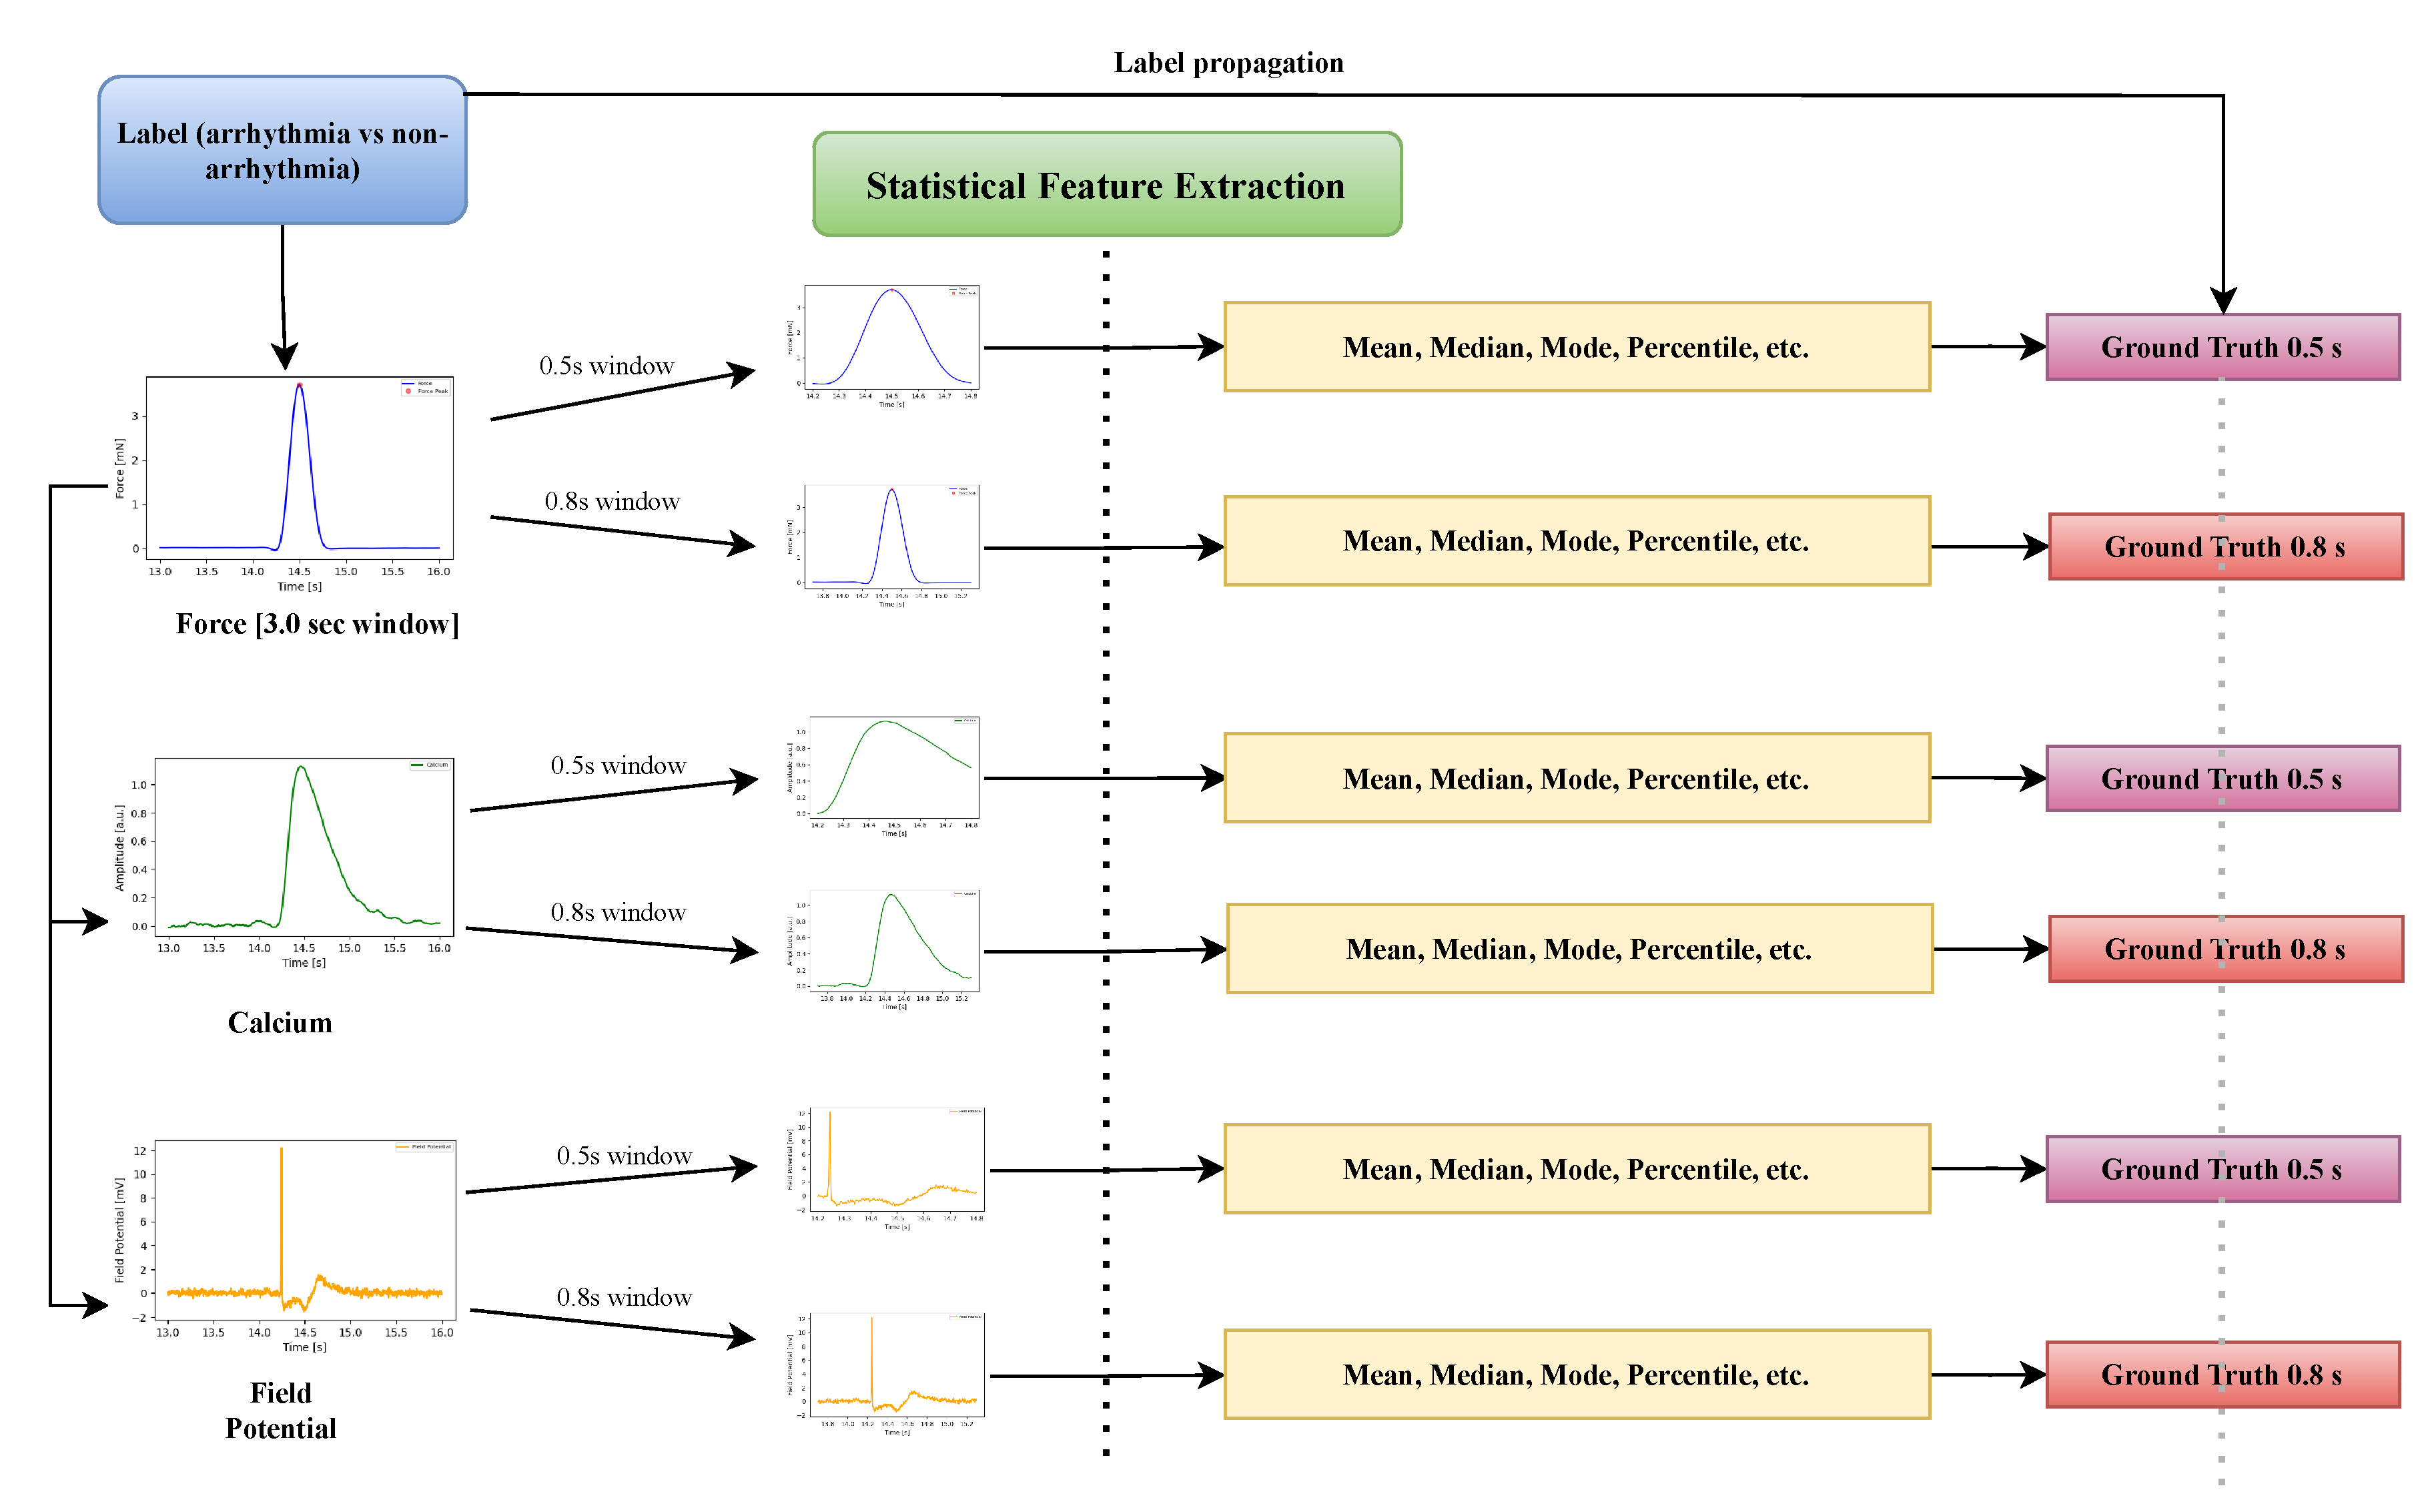
\includegraphics[width=1\textwidth, keepaspectratio]{plots/chapter_3/groundtruth-pipeline.drawio_new.pdf}
                \caption[Arrhythmia classification pipeline]{
                    \textbf{Arrhythmia classification pipeline} \par \small
                    Machine learning workflow: 
                    (1) Force-based peak detection, 
                    (2) 3s window extraction, 
                    (3) Manual labeling, 
                    (4) Window sub-division and TSFEL feature extraction (44 features), 
                    (5) Label Assignment,
                    (6) Random Forest Modeling (Balanced weights). 
                    Final models for Force and Calcium achieved F1=0.97 and F1=1.0 on arrhythmic and non-arrhythmic classes respectively, while for FP, best model achieved F1=0.99 and F1=1.0 for arrhythmic and non-arrhythmic events.}
                \label{fig:gt_workflow}
            \end{figure}
            
            Given the class imbalance (only 8\% of contractions were arrhythmic), Random Forest Classifiers with `balanced' weights were used for binary classification. Separate models were trained for each signal type and window size. The best test-set results were achieved with:
            \begin{itemize}
                \item A 2.4-second window model for force and calcium, achieving an \textbf{F1-score of 0.97 and 1.0} for arrhythmic and non-arrhythmic classes respectively.
                \item A 0.6-second window model for FP, achieving an \textbf{F1-score of 0.99 and 1.0} for arrhythmic and non-arrhythmic classes respectively.
            \end{itemize}
            
            For more details on modeling methodology and evaluation, refer to \textit{Section 4.5} of Arrhythmia Classification work \cite{Sarwar2024}.
            \subsection{Integration to current work}
            
            The trained arrhythmia detection models demonstrated high accuracy and generalizability, allowing for their integration into this thesis project. Before conducting further analysis, \textbf{all arrhythmic contractions were identified and removed} using these models, ensuring that only non-arrhythmic contractions were included in the dataset. This preprocessing step helped maintain data integrity and improved the robustness of subsequent analyses.


    \newpage
    \section{Feature Extraction}
        \label{feature-extraction}
        With preprocessed signals and accurately detected non-arrhythmic peaks, the next step involved extracting quantitative biomarkers that characterize tissue contraction strength, relaxation time, and electrical activity patterns. These features provide physiological insights into cardiac function and treatment-induced effects.
        
        \subsection{Biological Features from Force \& Calcium}
        \label{force-peak-detection}
            Features extracted from the force and calcium signals (Figure \ref{fig:force-related-features}) were computed using SciPy’s signal processing module, specifically the `peak\_widths' \cite{SciPy_peak_widths} function. This function, given the peak indices, signal values, and a relative height, determines the peak widths at that relative height with respect to peak amplitude. Additionally, it identifies the left and right intersection points of a horizontal line with the signal at a given relative height of the peak. These intersection points were further utilized to extract contraction and relaxation features. The extracted features are as follows:
            
            \begin{itemize}
                \item \textbf{Peak Amplitude}: The maximum signal value at the detected peak, measured in \SI{}{\textbf{\milli\newton}}
 for force and \textbf{arbitrary units (a.u.)} for calcium, respectively.
                \item \textbf{Peak Widths (0.2, 0.5, 0.8) [\SI{}{\textbf{\s}}]}: The signal width at relative \textbf{20\SI{}{\textbf{\percent}}}, \textbf{50\SI{}{\textbf{\percent}}}, and \textbf{80\SI{}{\textbf{\percent}}} of the peak height, measured in seconds (\SI{}{\textbf{\s}}).
                \item \textbf{Rise Time (RT 0.2-0.8) [\SI{}{\textbf{\s}}]}: The absolute time taken for the signal to rise from \textbf{20\SI{}{\textbf{\percent}} to 80\SI{}{\textbf{\percent}}} of the peak height, representing \textbf{contraction time}. Measured in seconds (\SI{}{\textbf{\s}}).
                \item \textbf{Rise Time (RT 0.8-Max) [\SI{}{\textbf{\s}}]}: The absolute time taken for the signal to rise from \textbf{80\SI{}{\textbf{\percent}} to peak amplitude}, measured in seconds (\SI{}{\textbf{\s}}).
                \item \textbf{Decay Time (DT Max-0.8) [\SI{}{\textbf{\s}}]}: The absolute time taken for the signal to decay from \textbf{peak amplitude to 80\SI{}{\textbf{\percent}}} of peak height, measured in seconds (\SI{}{\textbf{\s}}).
                \item \textbf{Decay Time (DT 0.2-0.8) [\SI{}{\textbf{\s}}]}: The absolute time taken for the signal to decay from \textbf{80\SI{}{\textbf{\percent}} to 20\SI{}{\textbf{\percent}}} of peak height, representing \textbf{relaxation time}. Measured in seconds (\SI{}{\textbf{\s}}).
            \end{itemize}

        
        \begin{figure}[H]
            \centering
            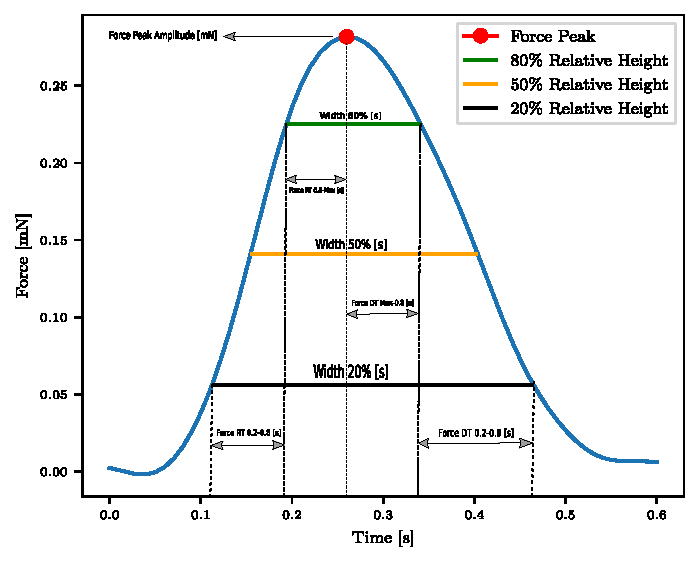
\includegraphics[ keepaspectratio]{plots/chapter_3/force-peak-widths-annotated.pdf}
               \caption[Biologically Relevant Feature Extraction for Force]{\textbf{Biologically Relevant Feature Extraction for Force.} This figure illustrates the key quantitative parameters extracted from the force signal, including peak amplitude (red), peak widths at 20\%, 50\%, and 80\% of the peak height (black, orange, green), rise times (RT\textsubscript{20-80}, RT\textsubscript{80-max}), and decay times (DT\textsubscript{max-80}, DT\textsubscript{20-80}). These parameters characterize contraction strength, timing, and relaxation dynamics. The same extraction approach applies to the calcium signal.}
    
            \label{fig:force-related-features}
        \end{figure}

        \subsection{Features from Field Potential}
        
            For the FP signal, two key features were extracted:
            
            \begin{itemize}
                \item \textbf{Field Potential Duration (FPD) [\SI{}{\textbf{\s}}]}: The absolute time difference (\SI{}{\textbf{\s}}) between the \textbf{Sodium (\(\text{Na}^+\)) peak} and the \textbf{T\(^+\) wave}, representing the \textbf{total duration of the contraction event}.
                \item \textbf{Local Frequency [\SI{}{\textbf{\hertz}}]}\footnote{The accuracy of this feature depends on the performance of the FP peak detection algorithm. If consecutive FP peaks are missed, the computed local frequency deviates from its intended definition, as it will measure time intervals between non-adjacent detected events. Improving the peak detection algorithm would enhance the reliability of this feature.}: Estimated using the time intervals between consecutive \textbf{Sodium (\(\text{Na}^+\)) peaks}, calculated as:
                \[
                \bm{f_{\text{local}}} = \frac{\bm{t_p + t_n}}{2 \cdot (\bm{t_p} \cdot \bm{t_n})}
                \]
                where \(\bm{t_p}\) and \(\bm{t_n}\) represent the time difference to the \textbf{previous} and \textbf{next} Sodium peak, respectively (measured in Hertz [Hz]). The formula is basically the reciprocal of \textit{harmonic mean} between two time periods, which provides a more appropriate averaging method for frequency-based measurements, as it better accounts for variations in peak intervals by reducing the influence of disproportionately large values. The \textbf{first and last detected peaks} were excluded from this calculation to avoid boundary effects (Figure \ref{fig:fp-definiton}).
            \end{itemize}

             \begin{figure}[H]
                \centering
                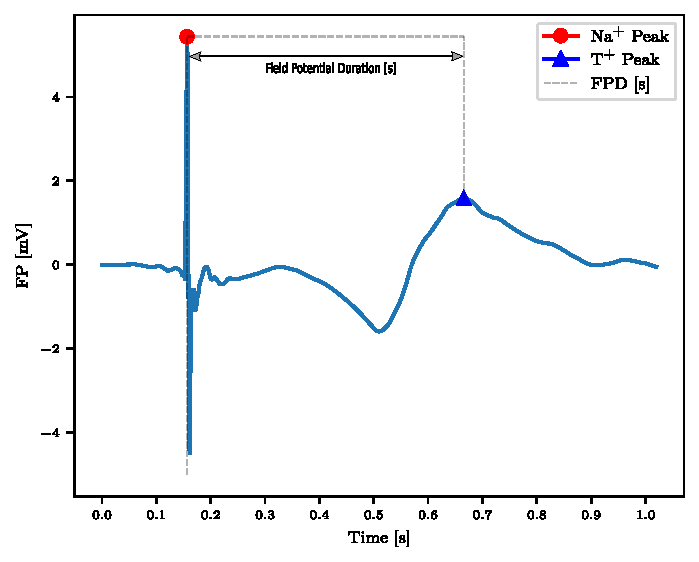
\includegraphics[width=0.6\textwidth]{plots/chapter_3/fp-duration-annotated.pdf}
                    \caption[Field Potential Duration Measurement]{\textbf{Field Potential Duration (FPD) Measurement.} The field potential duration (FPD) is computed as the time difference between the Na\textsuperscript{+} peak and the T\textsuperscript{+} wave in the FP signal. This measurement represents the total duration of a contraction event and serves as a key biomarker for assessing electrical activity and contraction timing.}
                \label{fig:fp-definiton}
            \end{figure}
        
        \begin{table}[H]
            \centering
            \caption{Summary of Extracted Features}
            \label{tab:features-summary}
            \begin{tabular}{l l l l}
                \toprule
                \textbf{Feature} & \textbf{Description} & \textbf{Signal Type} & \textbf{Unit} \\
                \midrule
                Peak Amplitude & Maximum peak value & Force, Calcium & \SI{}{\milli\newton}, a.u. \\
                Peak Width (0.2, 0.5, 0.8) & Width at 20\SI{}{\percent}, 50\SI{}{\percent}, 80\SI{}{\percent} peak height & Force, Calcium & \SI{}{\s} \\
                Rise Time (RT 0.2-0.8) & Time for 20\%-80\% peak rise & Force, Calcium & \SI{}{\s} \\
                Rise Time (RT 0.8-Max) & Time from 80\% to peak rise & Force, Calcium & \SI{}{\s} \\
                Decay Time (DT Max-0.8) & Time from peak to 80\% decay & Force, Calcium & \SI{}{\s} \\
                Decay Time (DT 0.2-0.8) & Time from 80\%-20\% decay & Force, Calcium & \SI{}{\s} \\
                Field Potential Duration (FPD) & Time between \(\text{Na}^+\) peak and \(\text{T}^+\) wave & Field Potential & \SI{}{\s} \\
                Local Frequency & Instantaneous beat frequency & Field Potential & \SI{}{\hertz} \\
                \bottomrule
            \end{tabular}
        \end{table}
        
        
        The extracted features across all signal types are summarized in Table~\ref{tab:features-summary}. To integrate extracted features across modalities, time alignment was performed based on detected peak indices. Specifically:
        \begin{itemize}
            \item Force and calcium peaks \textbf{co-occurring within the FPD of a detected field potential event} were linked to the corresponding field potential event.
            \item Any force or calcium peaks without an associated FP peak were excluded from the final dataset.
            \item  Likewise, FP peaks without corresponding force and calcium peaks were discarded.
        \end{itemize}
       
        This filtering ensured that the final dataset contained only fully matched contraction events, allowing for a coherent multimodal analysis of contraction dynamics. The resulting dataset was subsequently used for analyzing treatment-induced changes in tissue response quantified through the above extracted features.
        
        

\chapter{Data Mining and Analysis}
\label{analysis}
This chapter builds upon the rigorous preprocessing and feature extraction methodologies detailed in the preceding chapter, setting the stage for comprehensive data mining and analytical exploration of ECC responses. Having established robust datasets through careful preprocessing and feature extraction, this chapter leverages advanced analytical methods, including statistical hypothesis testing, dimensionality reduction (t-SNE), and regression-based modeling, to uncover meaningful biological insights from multimodal data. Specifically, the analysis systematically evaluates the effects of pharmacological stimulus—E-4031, Nifedipine, and Calcium titration experiments—on cardiac tissue functionality, elucidates dose-response relationships, assesses feature correlation dynamics, and identifies intricate treatment-induced feature associations. Collectively, these analyses aim to enhance understanding of treatment-induced modulation in ECC, reinforcing the utility of MTs as predictive human cardiac models.

\section{Global Overview}
    \label{global-overview}
    Following the extraction of biologically relevant features, the analysis began with establishing a global perspective of the dataset. A total of 18 features were extracted (Section \ref{feature-extraction}), and t-distributed Stochastic Neighbor Embedding (t-SNE) \cite{tsne} was applied to project high-dimensional feature representations of contraction events onto a 2D space, preserving local structure while reducing dimensionality. This aids in visualizing the data space at both treatment and concentration levels.

    \subsection{Data Projection to 2D Space}
    \label{sec:global-perp}
        As described in Section~\ref{sec:drugs}, the dataset consists of three different pharmacological treatments, each applied at varying concentrations\footnote{These pharmacological interventions exhibit sufficiently rapid onset within hiPSC-derived MTs, thereby eliminating the need for a formal washout period between concentrations and minimizing the risk of carry-over effects.}. The treatments and their respective concentrations are summarized in Table~\ref{tab:drug-concentrations}.

        \begin{table}[H]
            \centering
            \caption[Treatments and corresponding concentration levels]{
                Treatments and corresponding concentration levels. 
                * For Calcium Titration, the highest calcium concentration (\SI{4.0}{\umol}) was considered the baseline due to its distinct experimental nature. 
                For \textbf{Nifedipine}, a one-hour post-treatment condition (1h$_{pt}$) was included as a washout experiment to evaluate tissue recovery after drug removal. 
                Additional \textbf{E-4031} concentrations (\SI{0.1}{\umol} to \SI{1.0}{\umol}) were tested but discarded as all contractions were arrhythmic at these levels.
            }
            \label{tab:drug-concentrations}
            \begin{tabular}{l l}
                \toprule
                \textbf{Treatment} & \textbf{Concentration Levels (\SI{}{\textbf{\umol}})} \\
                \midrule
                \textbf{E-4031} & 0.003, 0.01, 0.03, 0.1, 0.3, 0.6, 1.0 \\
                \textbf{Nifedipine} & 0.01, 0.03, 0.1, 0.2, 0.3, 0.5, 1.0, 4.0, 10.0, 1h$_{pt}$ \\
                \textbf{Calcium Titration ($\bm{\text{Ca}^{2+}}$)} & 0.1, 0.2, 0.4, 0.6, 0.8, 1.0, 1.5, 2.0, 4.0* \\
                \bottomrule
            \end{tabular}
        \end{table}
        
        
        For \textbf{Nifedipine}, an additional condition referred to as \textbf{one-hour post-treatment (1h$_{pt}$)} was included in the dataset. This condition represents a \textbf{washout experiment}, where after the removal of the drug, measurements were taken one hour later. The purpose of this measurement is to assess whether the tissue recovers to its baseline state after drug exposure or if any residual effects persist. In the case of \textbf{E-4031}, an extended concentration range (\SI{0.1}{\umol} to \SI{1.0}{\umol}) was tested to investigate its effects at higher doses. However, at these concentrations, all contractions exhibited \textbf{arrhythmic behavior}, leading to their exclusion from further analysis. The retained concentration levels (\SI{0.003}{\umol} to \SI{0.03}{\umol}) were selected as they provided physiologically relevant responses without inducing complete arrhythmic activity.  Unlike E-4031 and Nifedipine, which were investigated for their dose-dependent effects, Calcium Titration primarily served to assess the influence of varying extracellular $\bm{\text{Ca}^{2+}}$ concentrations on contraction dynamics. The highest calcium \textbf{4.0} \SI{}{\textbf{\umol}} concentration was considered the baseline due to its distinct experimental nature compared to the other two drugs.

        
       Each drug was tested on two different tissues. To visualize the global feature space, features from all treatment concentrations were pooled before computing Scipy's  \cite{scikit-learn} t-SNE using default parameters (\textbf{perplexity = 30}, \textbf{iterations = 1000}). The resulting low-dimensional representation was averaged over contraction events per tissue and concentration, such that each point in Figure~\ref{fig:global-tsne} represents a unique combination of tissue and concentration. This visualization reveals structural relationships between contraction events across different experimental conditions.

    \subsection{Key Findings}
        A notable observation in Figure~\ref{fig:global-tsne} is the close proximity of contraction events for tissue \textbf{`1.20b\_B01'} under \textbf{E-4031 at 0.003 \SI{}{\textbf{\umol}}} and \textbf{$\bm{\text{Ca}^{2+}}$ at 2.0 \SI{}{\textbf{\umol}}} (from Calcium Titration) indicating a high degree of \textbf{feature similarity}. Further analysis of their feature distributions (Figure~\ref{fig:overlapping}) confirms that their values are closely aligned. This may be attributed to the fact that the same tissue was used in both experiments, leading to baseline-like feature distributions at these specific concentrations. Since 0.003  \SI{}{\umol} for E-4031 and 2.0  \SI{}{\umol} for $\bm{\text{Ca}^{2+}}$ are close to their respective baseline conditions, their contraction dynamics may exhibit similar characteristics. These findings highlight potential overlapping physiological effects, which could provide insight into alternative drug actions or shared mechanisms of action across treatments.

        Another key observation from this representation is that \textbf{different tissues exhibit distinct mean responses to drug exposure}, as shown by their spatial distribution in t-SNE space. This suggests potential tissue-specific variations in drug response, which may be relevant for identifying phenotypic differences across tissues and refining treatment strategies.



        \begin{figure}[H]
            \centering
            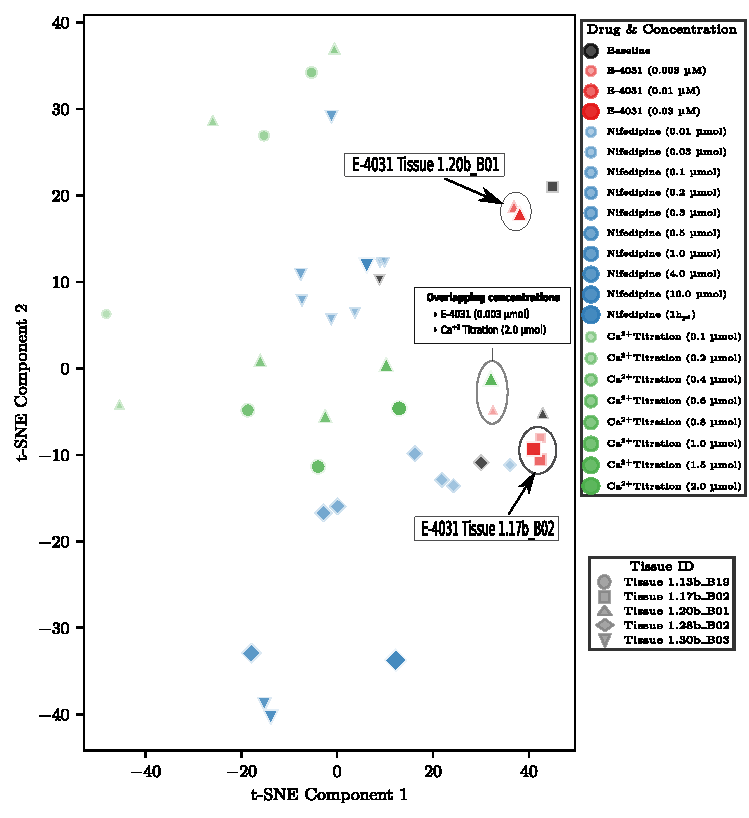
\includegraphics[width=1\textwidth, height=0.62\textheight,keepaspectratio]{plots/chapter_4/drug_wise_global_tsne_averaged_annotaed_2.pdf}
            \caption[Global t-SNE Projection of All Treatments and Concentrations (Perplexity = 30)]{
                \textbf{Global t-SNE Projection of All Treatments and Concentrations (Perplexity = 30)}:  
                This t-SNE visualization provides an overview of the feature space across all treatments and concentrations. Each point represents the averaged low-dimensional embedding for a unique tissue and treatment concentration combination. Proximity between points indicates similarity in feature distributions, highlighting potential physiological relationships. Notably, the overlap between contraction events under E-4031 (0.003  \SI{}{\umol}) and $\text{Ca}^{2+}$ from Calcium Titration (2.0  \SI{}{\umol}) for tissue `1.20b\_B01' suggests a high degree of feature similarity, possibly due to shared baseline-like characteristics. This finding may indicate similar mechanisms of action or alternative pharmacological effects, warranting further investigation. Additionally, distinct spatial separation between tissues highlights variations in their mean drug response (for instance, E-4031 `1.20b\_B01' and `1.17b\_B02' tissues, shown in red triangle and squares, respectively), suggesting potential tissue-specific effects that could be relevant for phenotypic characterization and treatment optimization.}
            \label{fig:global-tsne}
        \end{figure}

       \begin{figure}[H]
            \centering
            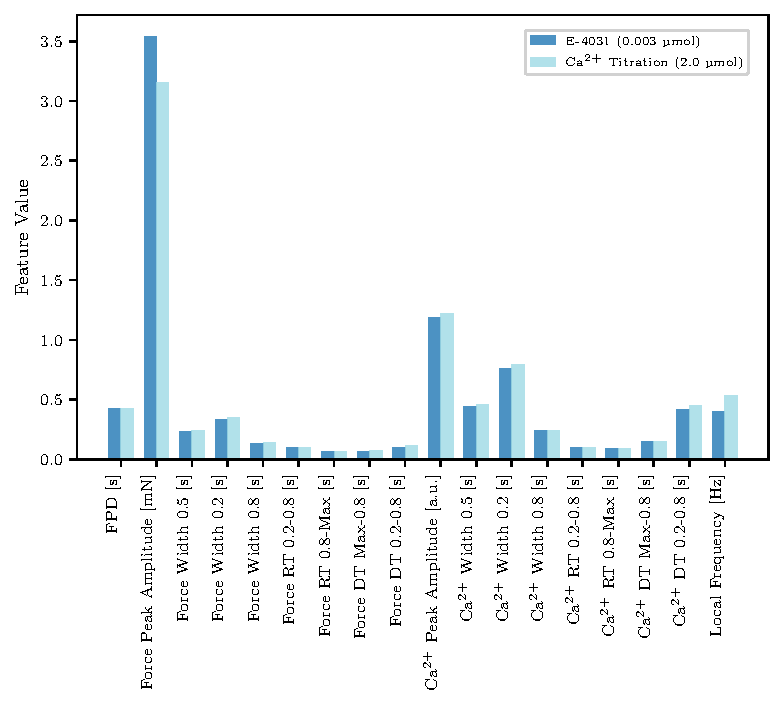
\includegraphics[width=0.8\textwidth, keepaspectratio]{plots/chapter_4/drug_tsne_overlapping_concentration.pdf}
            \caption[Feature Distribution for Overlapping E-4031 (0.003 \SI{}{\umol}) and Calcium Titration (2.0 \SI{}{\umol}) Concentrations]{
                \textbf{Feature Distribution for Overlapping E-4031 (0.003 \SI{}{\textbf{\umol}}) and Calcium Titration (2.0 \SI{}{\textbf{\umol}}) Concentrations}:  
                This plot displays the averaged feature values of contraction events recorded from tissue `1.20b\_B01' under two distinct treatment conditions--E-4031 (0.003 \SI{}{\umol}) and Calcium ($\text{Ca}^{2+}$) Titration (2.0 \SI{}{\umol}). Averaged representation from these conditions exhibited significant overlap in the t-SNE representation (Figure~\ref{fig:global-tsne}) and are also comparable in this plot. The similarity in feature values suggests that these conditions induce comparable physiological effects, potentially due to their proximity to baseline conditions. Such overlaps in feature space can help identify alternative treatment strategies or reveal shared pharmacodynamic mechanisms between drug treatments.}
            \label{fig:overlapping}
        \end{figure}

        \subsection{Section Summary}
        In summary, the t-SNE visualization provided a global perspective on treatment-induced contraction dynamics, revealing potential relationships between treatments and tissues. Notably, treatment conditions E-4031 (0.003 \SI{}{\umol}) and $\text{Ca}^{2+}$ (2.0 \SI{}{\umol}) from Calcium Titration experiment for tissue `1.20b\_B01' exhibited feature similarity, suggesting potential shared physiological effects. Additionally, distinct clustering across tissues highlighted potential tissue-specific variations in drug response, relevant for phenotypic characterization.

        % In the next section, a statistical analysis will be performed to further investigate the effects of drug treatments and quantify significant changes in contraction features.

    % \section{Drug-Level Perspective}  

    % To further drill down into the data space, t-SNE was performed at the drug level. For each drug, feature representations were computed, and t-SNE was applied using the default parameters (Section~\ref{sec:global-perp}). In this representation, each data point corresponds to the average t-SNE embedding of all contraction events for a given tissue and drug concentration combination. This averaging ensures that the representation reflects the overall response rather than individual fluctuations.  
    
    % A key observation from this representation is that \textbf{different tissues exhibit distinct mean responses to drug exposure}, as shown by their spatial distribution in t-SNE space. This suggests potential \textbf{tissue-specific variations in drug response}, which may be relevant for identifying phenotypic differences across tissues and refining treatment strategies.  
    
    % Figure~\ref{fig:nifedipine-tsne} presents the t-SNE projection for \textbf{Nifedipine}, illustrating how tissues respond at different drug concentrations. The corresponding t-SNE plots for \textbf{E-4031} and \textbf{$\bm{\text{Ca}^{2+}}$ titration} are available in the supplementary figures.  
    
    % \section{Drug-Level Perspective}
    %     To further investigate the structure of the dataset, t-SNE was performed at the drug level. Features from each drug were combined, and t-SNE was applied using the default parameters (Section \ref{sec:global-perp}). The t-SNE plots for \textbf{E-4031}, \textbf{Nifedipine}, and \textbf{$\bm{\text{Ca}^{2+}}$} are shown in Figures~\ref{fig:e4031-tsne},~\ref{fig:nifedipine-tsne}, and~\ref{fig:catitration-tsne}, respectively.
        
    %     At the drug level, data points from different tissues were highlighted using distinct markers to identify possible phenotypic variations. A key observation is that \textbf{tissues exhibit different clustering behaviors across drug concentrations}, which may indicate tissue-specific responses to drug exposure. This differentiation is particularly relevant in identifying variations in phenotypic response and may assist in refining personalized treatment strategies.


    % \begin{figure}
    %     \centering
    %     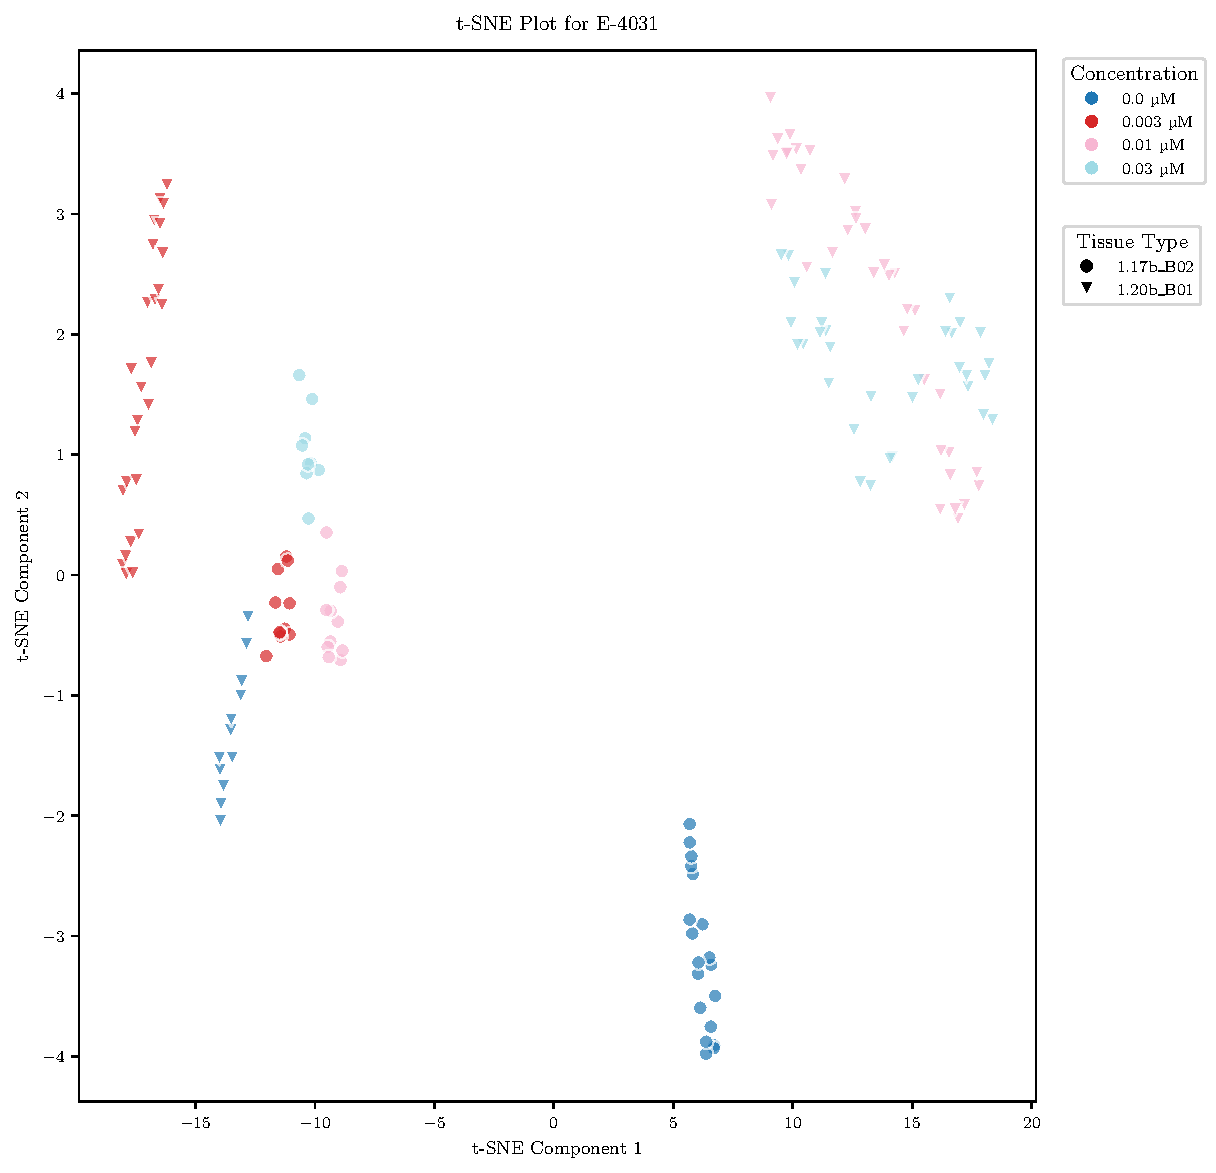
\includegraphics[width=0.8\textwidth, keepaspectratio]{plots/chapter_4/e4031_plot.pdf}
    %     \caption[t-SNE Projection of Feature Space for E-4031 Treatment (Perplexity = 30)]{\textbf{t-SNE Projection of Feature Space for E-4031 Treatment (Perplexity = 30)}:
    %     This plot visualizes the feature space distribution for samples treated with different concentrations of E-4031.}
    %     \label{fig:e4031-tsne}
    % \end{figure}

        % \begin{figure}[H]
        %     \centering
        %     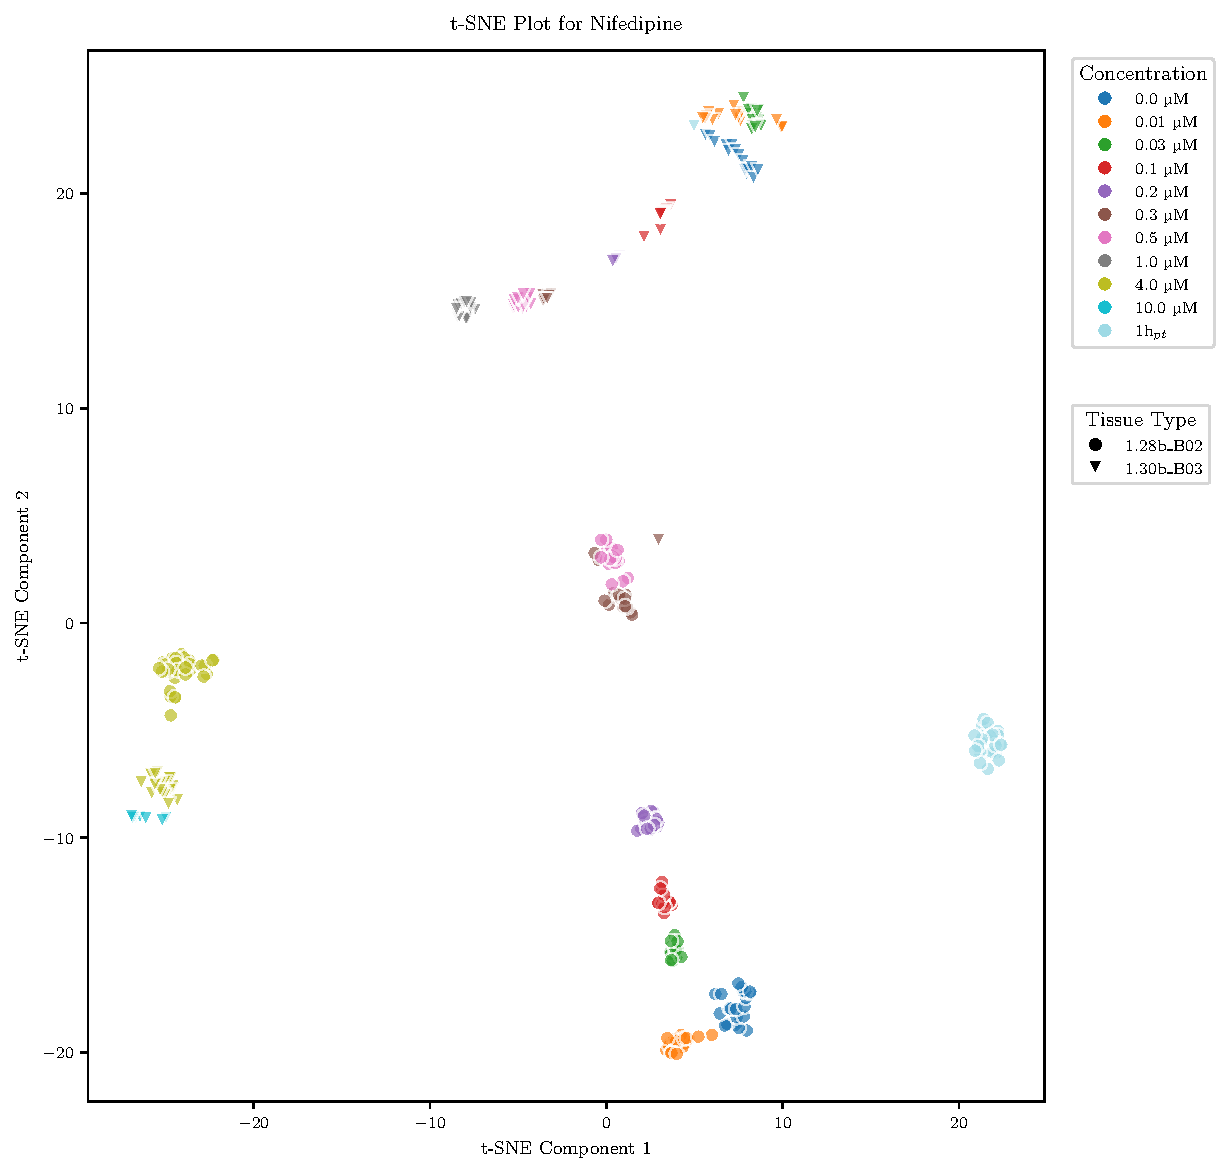
\includegraphics[width=0.8\textwidth, keepaspectratio]{plots/chapter_4/nifedipine_plot.pdf}
        %     \caption[t-SNE Projection of Feature Space for Nifedipine Treatment (Perplexity = 30)]{\textbf{t-SNE Projection of Feature Space for Nifedipine Treatment (Perplexity = 30)}:
        %     This plot visualizes the feature space distribution for samples treated with different concentrations of Nifedipine.}
        %     \label{fig:nifedipine-tsne}
        % \end{figure}

    % \begin{figure}
    %     \centering
    %     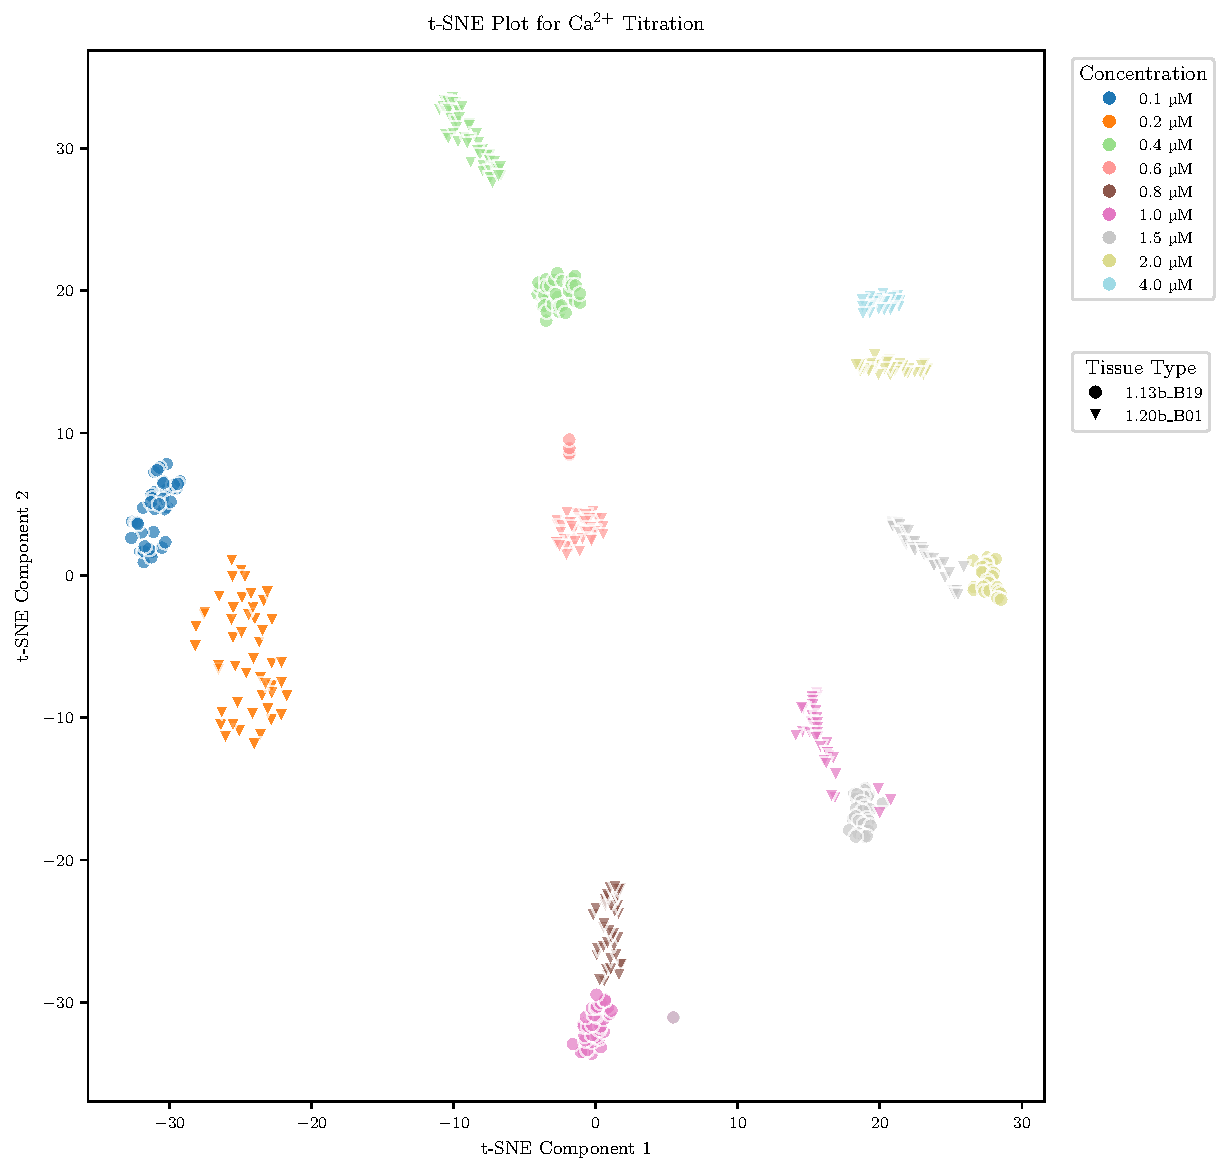
\includegraphics[width=1.0\textwidth, keepaspectratio]{plots/chapter_4/ca_titration_plot.pdf}
    %     \caption[t-SNE Projection of Feature Space for Calcium Titration Experiment (Perplexity = 30)]{\textbf{t-SNE Projection of Feature Space for Calcium Titration Experiment (Perplexity = 30)}:
    %     This plot visualizes the feature space distribution for samples treated with different concentrations of Calcium.}
    %     \label{fig:catitration-tsne}
    % \end{figure}

\section{Statistical Analysis of Treatment Effects} 
    \label{chap:statistical_analysis}

    Having established a global overview of the data space, the next crucial step was to determine the statistically significant effects of pharmacological treatments. This analysis was conducted at both the overall treatment level and the concentration level using mixed modeling and post-hoc tests, respectively. Specific hypotheses regarding known treatment effects, previously presented in the literature (see Literature Review, Chapter \ref{literature}; \cite{Kawatou2017-gh, Min2024-nc}), were reformulated and systematically evaluated.

    
    \subsection{E-4031} 
    \label{e4031-significance-analysis}
        \subsubsection{Methodology}
        \label{e4031-met}
            E-4031, known to induce arrhythmias at higher concentrations, was tested. Measurements from higher concentrations were discarded in the arrhythmia classification study (Section~\ref{sec:arrythmia}), leaving only data from three concentrations and baseline. A summary of available data is shown  in Table \ref{tab:e4031}. Since measurements were available for both tissues at each concentration, a crossed design\footnote{A \textbf{crossed design} in statistical modeling refers to an experimental setup where each level of one factor appears in combination with all levels of another factor \cite{nestedcrossed}.} with repeated measures\footnote{As each tissue is repeatedly exposed to multiple concentrations, its a repeated measure design.} was employed. To account for tissue variability, a mixed-effects model was used, treating tissue as a random effect while keeping concentration as a fixed effect\footnote{A \textbf{fixed effect} represents a factor whose levels are of direct interest and are assumed to be consistent across different samples, while a \textbf{random effect} is a factor whose levels are drawn from a larger population and introduce variability that is accounted for in the model. \cite{WikipediaMixedModel}}. This approach improves control of the Type I error rate and increases statistical power, leading to more accurate inference. The model decomposes error variation into two components: one due to tissue variability ($\sigma_\alpha$) and the other due to measurement residuals ($\sigma_\epsilon$).
            
            The model was fitted using the \texttt{lmerTest} \cite{lmertest} package in R and is expressed as:
            \[
            Y = \beta_0 + \beta_1 \cdot [\text{Concentration}] + Z_\alpha \cdot \text{[Tissue ID]} + \epsilon,
            \]
            where:
            \begin{itemize}
                \item \(Y\) is the target feature.
                \item \(\beta_0\) is the intercept, capturing the overall mean response.
                \item \(\beta_1\) is the fixed effect of concentration and is the primary effect of interest in this analysis, capturing the direct influence of concentration on the feature response (i.e. \(Y\)). \text{[Concentration]} is the corresponding factor variable\footnote{A \textbf{factor variable} is a categorical variable with a fixed set of levels, used in statistical models to represent group differences where one level is typically chosen as the \textbf{reference category (baseline)} for comparison.} with four levels (baseline and 3 concentrations).
                \item \(Z_\alpha\) represents the random effect (a.k.a random intercept) of tissue, modeled as a normally distributed variable: i.e \(Z_\alpha \sim \mathcal{N}(0, \sigma_\alpha^2)\). The variable \text{[Tissue ID]} is the  2-level factor distinguishing different tissues. Since $Z_\alpha$ is a random effect, the model estimates its variance $\sigma_\alpha^2$ rather than individual $Z_\alpha$ values.
                \item \(\epsilon\) is the error term, with \(\epsilon \sim \mathcal{N}(0, \sigma_\epsilon^2)\).
            \end{itemize}
            
            For post-hoc analyses, the Dunnett's test \cite{WikipediaDunnettTest} was used to compare concentration levels with the baseline. This test adjusts the significance level for multiple comparisons and was implemented using the \texttt{multcomp} \cite{multcomp} package in R. The significance level was set to 0.05.
            
            The results for a subset of features are shown in Figure~\ref{fig:sig_subset_e4031}. For each feature, the global p-value\footnote{Statistical significance of \(\beta_1\).} (with Welch's correction) is displayed at the top of the plot, along with the decomposition of error variance into \(\sigma_\alpha\) and \(\sigma_\epsilon\). This global p-value indicates whether the treatment has a statistically significant effect on feature response compared to the baseline, with a significant value suggesting that the treatment induces measurable changes beyond natural variability. The fit's singularity (or non-singularity) is also indicated. A singular fit occurs when the estimated value of \(\sigma_\alpha\) is zero. Welch's correction \cite{WikipediaWelchSatterthwaite} was applied to adjust for heteroscedasticity\footnote{\textbf{Heteroscedasticity} refers to the condition where the variance of the errors in a regression model is not constant across observations, potentially violating model assumptions and affecting inference.} (unequal variances between tissues), which was observed in residual diagnostics (Figure~\ref{fig:fit_v_residual_subset_e4031}). This ensures more reliable significance testing despite violating the homoscedasticity (equal variance) assumption. For example, the \textit{\(\text{Ca}^{2+}\)Peak Amplitude} feature exhibits heteroscedasticity, with residuals increasing as fitted values increase, following a funnel-shaped pattern.
            
            The p-values from the Dunnett's test are shown as horizontal significance lines above each concentration on the x-axis, where "ns" indicates non-significance and asterisks (*) indicate significance compared to the baseline. The significance levels are: * \(p < 0.05\), ** \(p < 0.01\), *** \(p < 0.001\). A significant p-value for a concentration indicates a statistically significant deviation in feature response at that concentration of treatment compared to the baseline. If the global p-value is not significant, no post-hoc concentration-level tests are performed (as for \textit{\(\text{Ca}^{2+}\)Peak Amplitude}).
            
            The Quantile-Quantile (QQ) plots of residuals for each feature (Figure~\ref{fig:qq_subset_e4031}) were used to assess the residuals normality assumption. While some residuals deviate slightly from normality, linear mixed models are known to be robust to such deviations \cite{jacqmingadda:inserm-00084214}, and the residuals are not excessively non-normal. Results for additional features are provided in the supplementary figures (Figures \ref{fig:e4031-remaining-significance}--\ref{fig:e4031-remaining-resid}).
            

           \begin{table}[H]
                \centering
                \caption{Contraction event counts across E-4031 concentrations (Crossed Design).}
                \label{tab:e4031}
                \begin{tabular}{p{2.5cm} @{\hskip 6pt} cccc | c}
                    \toprule
                    \multirow{2}{*}{\textbf{Tissue ID}} & \multicolumn{4}{c|}{\textbf{E-4031 Concentration (\SI{}{\textbf{\umol}})}} & \multirow{2}{*}{\textbf{Total}} \\
                    \cmidrule(lr){2-5}
                     & \textbf{0.0} & \textbf{0.003} & \textbf{0.01} & \textbf{0.03} &  \\
                    \midrule
                    1.17b\_B02 & 19  & 11  & 11  & 9   & 50 \\
                    1.20b\_B01 & 12  & 26  & 35  & 32  & 105 \\
                    \midrule
                    \textbf{Total} & 31  & 37  & 46  & 41  & \textbf{155} \\
                    \bottomrule
                \end{tabular}
            \end{table}
            
    
            \begin{figure}[h]
                \centering
                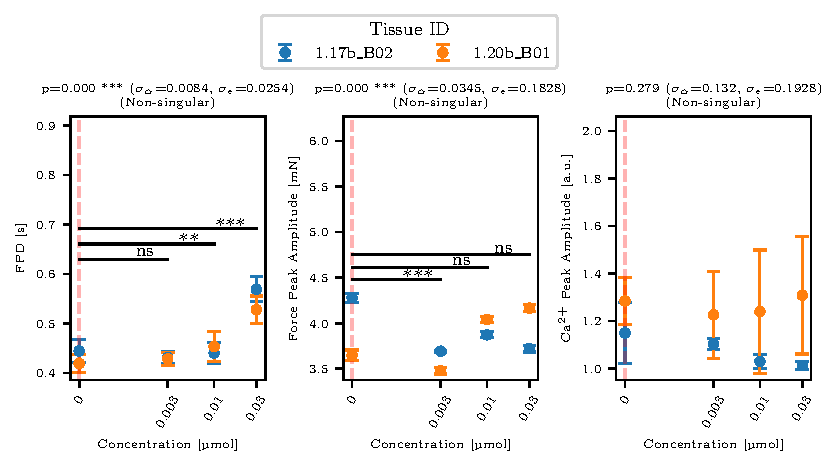
\includegraphics[width=1.0\textwidth, keepaspectratio]{plots/chapter_5/e4031/significance_features_lmer_subset_3.pdf}
                \caption[Statistical significance of E-4031 treatment on subset of Biological features.]{\textbf{Statistical significance of E-4031 treatment on subset of Biological features}:  
                This figure presents the results of a mixed-effects model assessing the impact of E-4031 on a subset of biological features, controlling for tissue-specific variability through inclusion of a random-effect. Global p-values (with Welch's correction for heteroscedasticity) are shown atop each subplot, while horizontal significance lines (from post-hoc Dunnett’s tests) compare each treatment concentration with baseline (orange, dotted). Significance is indicated as * \(p < 0.05\), ** \(p < 0.01\), *** \(p < 0.001\), and "ns" denotes non-significance. Additionally, each subplot displays the estimated decomposition of error variance into tissue variability (\(\sigma_\alpha\)) and residual noise (\(\sigma_\epsilon\)). The hypothesis that increasing E-4031 concentration leads to a significant increase in field potential duration (FPD) is strongly supported by these results (\textit{FPD} **\(p < 0.01\) and ***\(p < 0.001\) for 0.01 \SI{}{\umol} and 0.03 \SI{}{\umol} respectively.)}
            
                \label{fig:sig_subset_e4031}
            \end{figure}
        
            \begin{figure}[h]
                \centering
                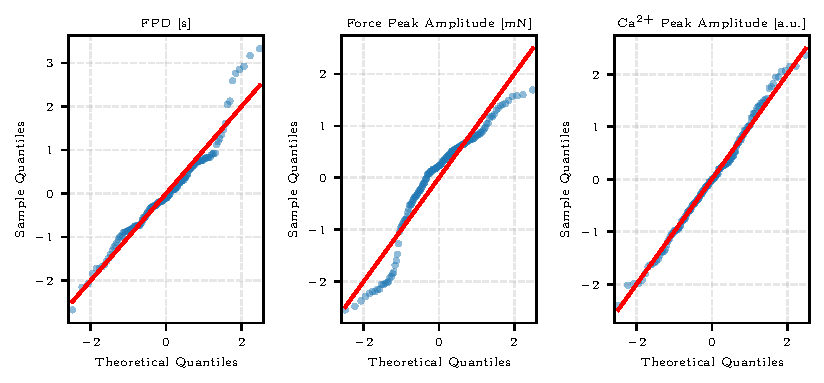
\includegraphics[width=1.0\textwidth, keepaspectratio]{plots/chapter_5/e4031/qq_mixed_subset_3.pdf}
                \caption[QQ Plot of Residuals for Mixed Model Fit of E-4031 Treatment.]{\textbf{QQ Plot of Residuals for Mixed Model Fit of E-4031 Treatment.}: This QQ plot evaluates the normality of residuals from the mixed-effects model. Although some deviation from the normal line is apparent, linear mixed models are robust to such deviations  \cite{jacqmingadda:inserm-00084214}.}
                \label{fig:qq_subset_e4031}
            \end{figure}
        
            \begin{figure}[H]
                \centering
                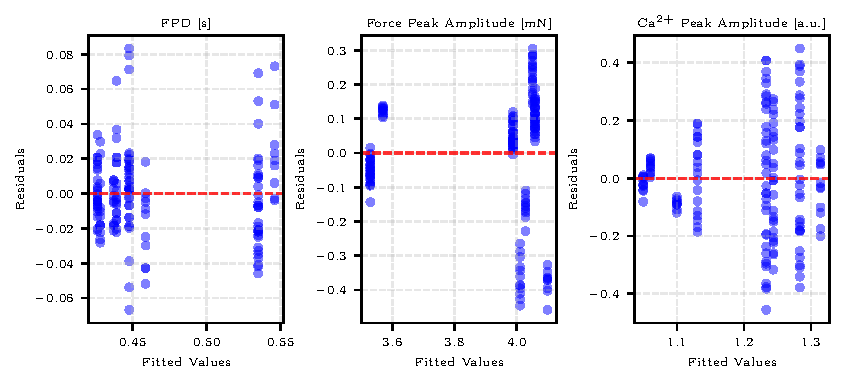
\includegraphics[width=1\textwidth, keepaspectratio]{plots/chapter_5/e4031/resid_mixed_subset_3.pdf}
                \caption[Residuals vs. Fitted Values for Mixed Model Fit of E-4031 Treatment]{\textbf{Residuals vs. Fitted Values for Mixed Model Fit of E-4031 Treatment}: This diagnostic plot shows the relationship between residuals and fitted values. A funnel-shaped pattern in \textit{\(\text{Ca}^{2+}\)Peak Amplitude} indicates heteroscedasticity, which was addressed via Welch's correction during significance testing.}
                \label{fig:fit_v_residual_subset_e4031}
            \end{figure}
        \subsubsection{Hypothesis Evaluation}
            The hypothesis for E-4031 is that it increases field potential duration (FPD) at lower concentrations, ultimately inducing arrhythmia's at higher concentrations. Thus, the hypothesis statement is:
            \[
            \text{The field potential duration (FPD) should increase significantly with increasing E-4031 concentration.}
            \]
            
            As shown in Figure~\ref{fig:sig_subset_e4031}, the overall drug effect on field potential duration (FPD) is highly significant (\(p < 0.001\)). Post-hoc analysis reveals that concentrations of 0.01 \SI{}{\umol} and 0.03 \SI{}{\umol} significantly increase FPD compared to baseline (\(p < 0.01\) and \(p < 0.001\), respectively). This confirms the hypothesis, demonstrating that E-4031 significantly impacts FPD as E-4031 concentration increases.
        
    \subsection {Nifedipine} 
     \label{nifedipine-significance-analysis}
        \subsubsection{Methodology}
            \label{nifedipine-sig-methodology}
            For Nifedipine, measurements were not available for all concentrations in both tissues (Table~\ref{tab:nifedipine}), resulting in a nested design\footnote{A \textbf{nested design} is an experimental setup where the levels of one factor are unique to each level of another factor, meaning they do not repeat across different levels of the higher-order factor \cite{nestedcrossed}.}. To account for this, a nested random effect\footnote{The model design was motivated from this StackExchange \href{https://stats.stackexchange.com/questions/630358/how-to-handle-pseudoreplication-aggregate-observations-per-group-for-linear-mi?fbclid=IwY2xjawHCF1hleHRuA2FlbQIxMAABHcBmtcQyzFZ_QiBUKlHD6kRFqbgdVj-UZTF8316U_KKMeWe5sUYCXl0TwQ_aem_qwBMa6uYIez1NB2aRHz5vQ}{thread}.} for concentration within tissue was added to the model:
            \[
            Y = \beta_0 + \beta_1 \cdot [\text{Concentration}] + Z_\alpha \cdot \text{[Tissue ID]} + Z_\beta \cdot [\text{Tissue ID:Concentration}] + \epsilon,
            \]
            where:
            \begin{itemize}
                \item \(Z_\beta\) is the random effect of concentration nested within tissue, with \(Z_\beta \sim \mathcal{N}(0, \sigma_\beta^2)\). Since nested effects are modeled as random, the model estimates only the variance of the nested effect $\sigma_\beta^2$, rather than individual values $Z_\beta$.
                \item \text{[Tissue ID:Concentration]} is a factor variable that uniquely identifies each combination of tissue and its corresponding concentrations. Based on the Nifedipine data structure (Table ~\ref{tab:nifedipine}), the number of levels for this nested effect is 20, considering that 9 concentrations are applied to both tissues, while 2 concentrations (1 \SI{}{\umol} and 10 \SI{}{\umol}) are exclusive to tissue 1.30b\_B03.
            \end{itemize}
            
            The methodology otherwise remains consistent with the E-4031 analysis. Significance results for a subset of features are shown in Figure~\ref{fig:sig_subset_nifedipine}. The results for remaining features along with their diagnostic plots are provided in the supplementary figures (Figures \ref{fig:nifedipine-remaining-significance}--\ref{fig:nifedipine-remaining-resid}).
            

            \begin{table}[H]
                \centering
                \caption{Contraction event counts across Nifedipine concentrations (Nested Design).}
                \label{tab:nifedipine}
                \begin{tabular}{p{2.5cm} @{\hskip 6pt} ccccccccccc | c}
                    \toprule
                    \multirow{2}{*}{\textbf{Tissue ID}} & \multicolumn{11}{c|}{\textbf{Nifedipine Concentration (\SI{}{\textbf{\umol}})}} & \multirow{2}{*}{\textbf{Total}} \\
                    \cmidrule{2-12}
                     & \textbf{0.0} & \textbf{0.01} & \textbf{0.03} & \textbf{0.1} & \textbf{0.2} & \textbf{0.3} & \textbf{0.5} & \textbf{1.0} & \textbf{4.0} & \textbf{10.0} & \textbf{1h$_{pt}$} &  \\
                    \midrule
                    1.28b\_B02 & 24  & 18  & 15  & 15  & 19  & 16  & 19  & 0   & 32  & 0   & 29  & 187 \\
                    1.30b\_B03 & 16  & 16  & 16  & 13  & 11  & 10  & 15  & 19  & 24  & 9   & 1   & 150 \\
                    \midrule
                    \textbf{Total} & 40  & 34  & 31  & 28  & 30  & 26  & 34  & 19  & 56  & 9   & 30  & \textbf{337} \\
                    \bottomrule
                \end{tabular}
            \end{table}
    
            \begin{figure}[H]
                \centering
                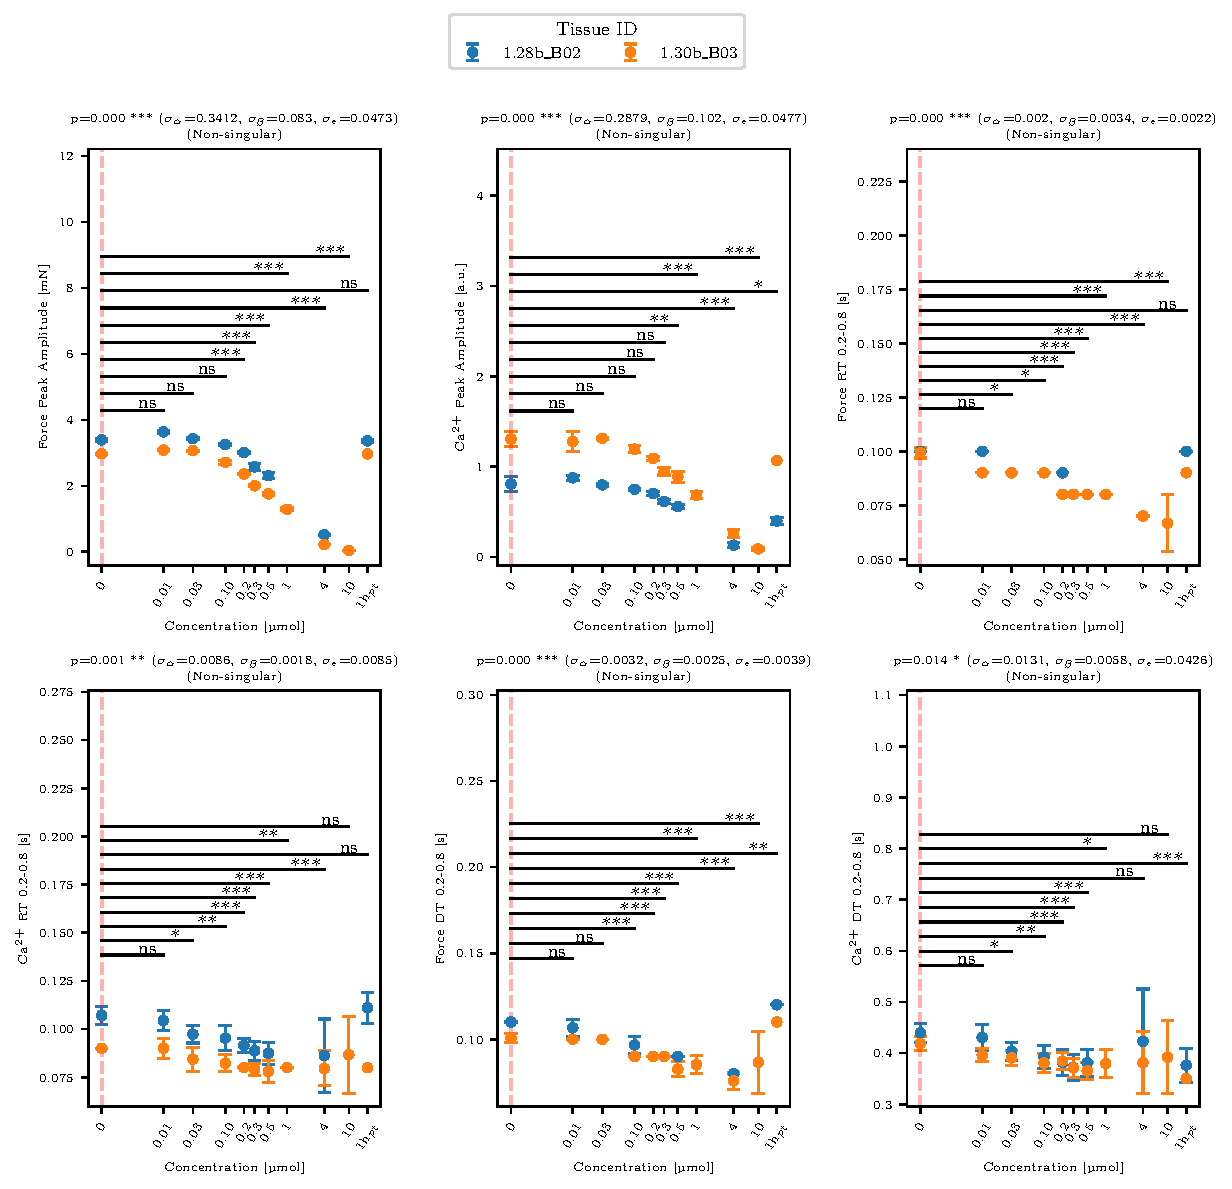
\includegraphics[width=1.0\textwidth, keepaspectratio]{plots/chapter_5/nifedipine/significance_features_lmer_subset_6.pdf}
                \caption[Statistical significance of Nifedipine treatment on subset of Biological features.]{\textbf{Statistical significance of Nifedipine treatment on subset of Biological features.}: This figure presents the results of an extended mixed-effects model, incorporating a nested design to account for concentration effects within tissues. Global p-values (with Welch’s correction) are displayed on-top of each feature, with post-hoc Dunnett’s test comparisons (denoted by * \(p < 0.05\), ** \(p < 0.01\), *** \(p < 0.001\), and “ns” for non-significance) marking significant differences from baseline. Both force and calcium peak amplitudes, as well as contraction and relaxation times (e.g., \textit{Force RT 0.2–0.8, Ca\(^{2+}\) RT 0.2–0.8, Force DT 0.2–0.8}, and \textit{Ca\(^{2+}\) DT 0.2–0.8}), are shown in the plot. The estimated variance for the nested concentration effect (\(\sigma_\beta\)) is also provided on top. These results confirm that increasing Nifedipine concentrations significantly reduce peak amplitudes and shorten contraction and relaxation durations, supporting the hypothesis that Nifedipine weakens contractions by disrupting calcium-dependent ECC (*** \(p < 0.001\) for \textit{Force Peak Amplitude} \& \textit{Calcium Peak Amplitude} at 0.2–10 \SI{}{\umol} and 1–10 \SI{}{\umol} respectively. Contraction and Relaxation features also show significant decline at increasing concentrations of Nifedipine.)}
                \label{fig:sig_subset_nifedipine}
            \end{figure}
        
            % \begin{figure}
            %     \centering
            %     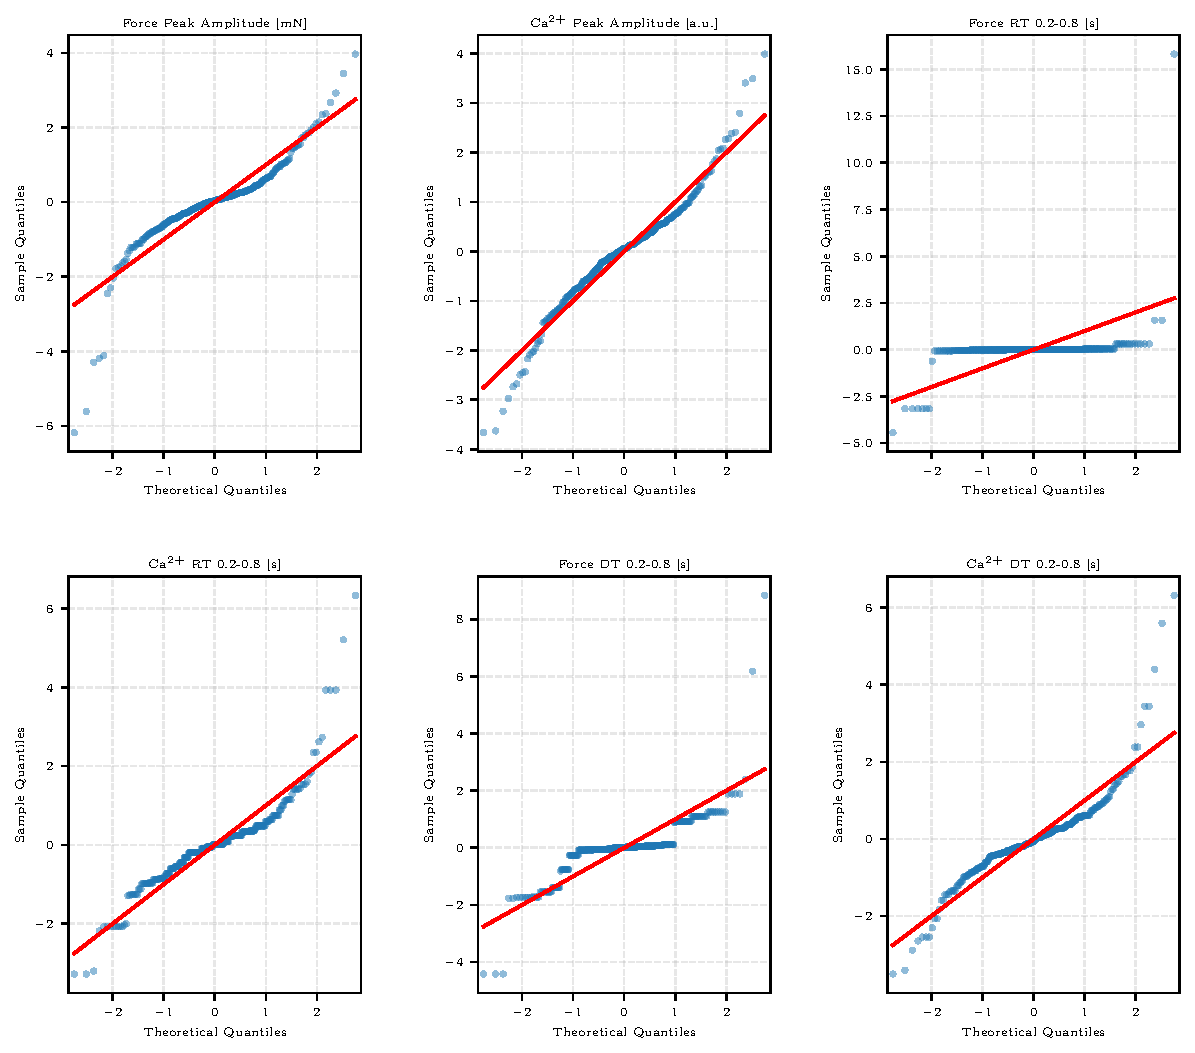
\includegraphics[width=1.0\textwidth, keepaspectratio]{plots/chapter_5/nifedipine/qq_mixed_subset_6.pdf}
            %     \caption[QQ Plot of Residuals for Mixed Model Fit of Nifedipine Treatment.]{\textbf{QQ Plot of Residuals for Mixed Model Fit of Nifedipine Treatment.}}
            %     \label{fig:qq_subset_nifedipine}
            % \end{figure}
        
            % \begin{figure}
            %     \centering
            %     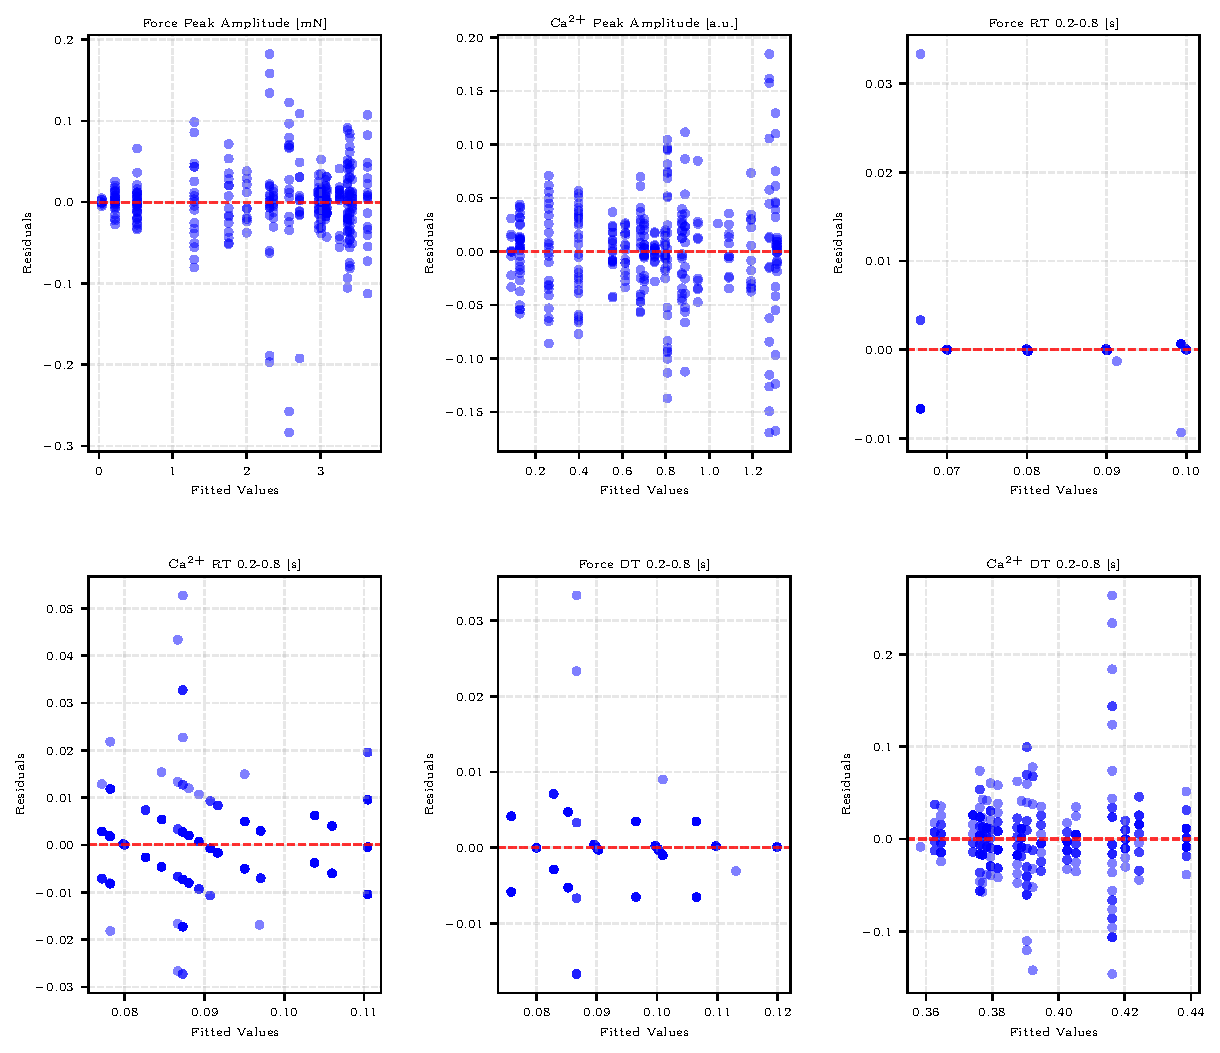
\includegraphics[width=0.9\textwidth, keepaspectratio]{plots/chapter_5/nifedipine/resid_mixed_subset_6.pdf}
            %     \caption[Residuals vs. Fitted Values for Mixed Model Fit of Nifedipine Treatment.]{\textbf{Residuals vs. Fitted Values for Mixed Model Fit of Nifedipine Treatment.}}
            %     \label{fig:fit_v_residual_subset_nifedipine}
            % \end{figure}
    
            % \begin{figure}[H]
            %     \centering
            %     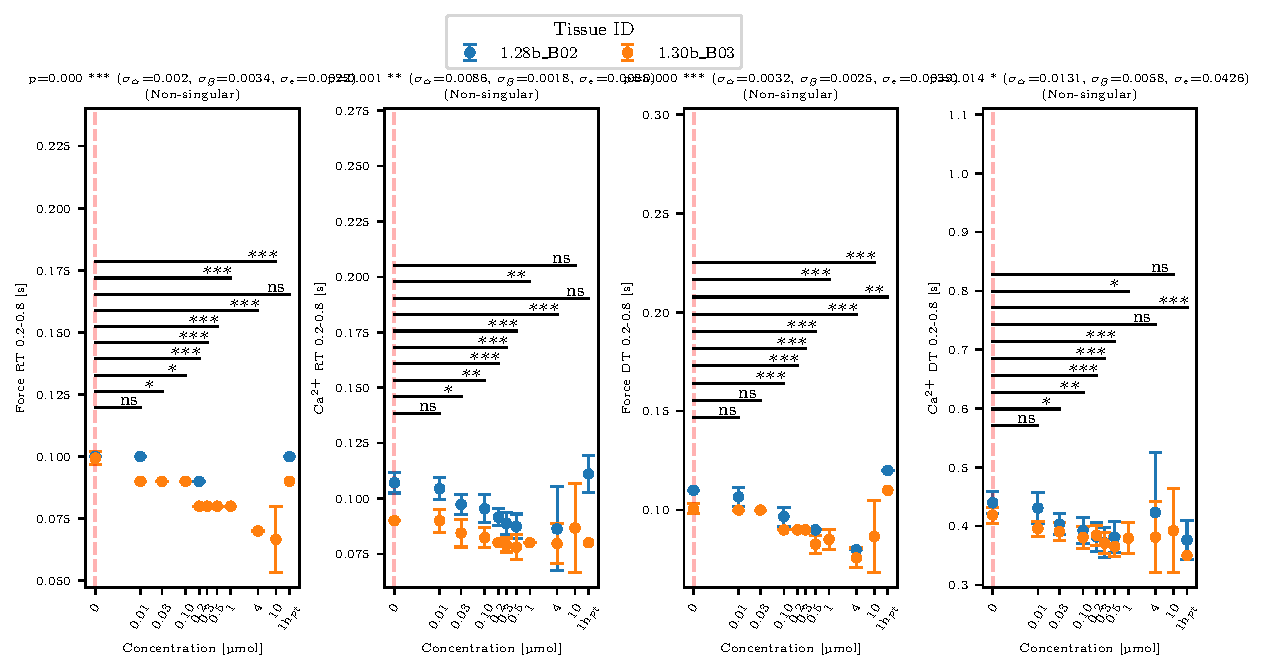
\includegraphics[width=1.0\textwidth, keepaspectratio]{plots/chapter_5/nifedipine/significance_features_lmer_subset_4.pdf}
            %     % \caption[Nifedipine’s Effects on Contraction and Relaxation Features.]{\textbf{Nifedipine’s Effects on Contraction and Relaxation Features.}: 
            %     % This figure provides a focused analysis of Nifedipine’s impact on contraction and relaxation dynamics in cardiac tissues. The results confirm that increasing concentrations of Nifedipine significantly reduce contraction duration and relaxation duration, consistent with its role in inhibiting calcium-dependent excitation-contraction coupling.}
            %     \label{fig:sig_subset_hypothesis_nifedipine}
            % \end{figure}
            
        \subsubsection{Hypothesis Evaluation}
            Nifedipine, a calcium channel blocker, weakens contractions by disrupting the calcium-induced calcium release (CICR) cycle. The hypothesis is:
            \begin{quote}
                The amplitude of calcium and force, as well as tissue contraction and relaxation times, should decrease with increasing Nifedipine concentration.
            \end{quote}
            
            
            As shown in Figure~\ref{fig:sig_subset_nifedipine}, the force peak and calcium peak amplitudes decrease significantly with increasing Nifedipine concentration (\(p < 0.001\)). Post-hoc analysis indicates that concentrations of 0.2–10 \SI{}{\umol} and 1–10 \SI{}{\umol} significantly reduce force and calcium peak amplitudes compared to baseline. Similarly, features representing tissue contraction and relaxation times (e.g., \textit{Force RT 0.2–0.8, Ca$^{+2}$ RT 0.2–0.8, Force DT 0.2-0.8} and \textit{Ca$^{+2}$ DT 0.2-0.8)} also show significant decreases. These results confirm the hypothesis, demonstrating that Nifedipine weakens contractions and reduces tissue contraction and relaxation times.
            
        
   \subsection{Calcium Titration Experiment}
    \label{ca-significance-analysis}
        \subsubsection{Methodology}
           The methodology for the calcium titration experiment follows the same design as the Nifedipine experiment, using a nested design approach (Table~\ref{tab:ca_titration}). In this context, \textit{Force Peak Amplitude} is the only relevant feature for hypothesis evaluation due to its sensitivity to changes in calcium concentrations, making it a key indicator of the physiological response in this experiment. The result for \textit{Force Peak Amplitude} is shown in Figure~\ref{fig:sig_subset_ca_titration}.

            
            \subsubsection{Hypothesis Evaluation}
            The hypothesis for the calcium titration experiment is straightforward:
            \[
            \text{Increasing calcium concentration enhances contractile force.}
            \]
            
            As shown in Figure~\ref{fig:sig_subset_ca_titration}, the force peak amplitude increases significantly with calcium concentration (\(p < 0.001\)), confirming the hypothesis.
    

        
            \begin{table}[H]
                \centering
                \caption{Contraction event counts across Calcium Titration experiment concentrations (Nested Design).}
                \label{tab:ca_titration}
                \begin{tabular}{p{2.5cm} @{\hskip 6pt} ccccccccc | c}
                    \toprule
                    \multirow{2}{*}{\textbf{Tissue ID}} & \multicolumn{9}{c|}{\textbf{Calcium Concentration (\SI{}{\textbf{\umol}})}} & \multirow{2}{*}{\textbf{Total}} \\
                    \cmidrule{2-10}
                     & \textbf{4.0} & \textbf{0.1} & \textbf{0.2} & \textbf{0.4} & \textbf{0.6} & \textbf{0.8} & \textbf{1.0} & \textbf{1.5} & \textbf{2.0} &  \\
                    \midrule
                    1.13b\_B19 & 0  & 40  & 0  & 35  & 9  & 0  & 34  & 31  & 25  & 174 \\
                    1.20b\_B01 & 22  & 0  & 98  & 47  & 37  & 39  & 36  & 33  & 32  & 344 \\
                    \midrule
                    \textbf{Total} & 22  & 40  & 98  & 82  & 46  & 39  & 70  & 64  & 57  & \textbf{518} \\
                    \bottomrule
                \end{tabular}
            \end{table}
    
    
            \begin{figure}[H]
                \centering
                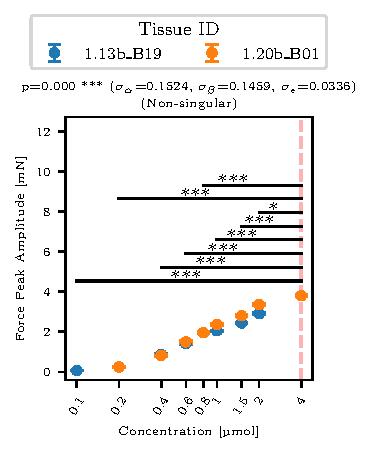
\includegraphics[width=0.5\textwidth, keepaspectratio]{plots/chapter_5/ca_titration/significance_features_lmer_subset_1.pdf}
                    \caption[Statistical significance of Calcium Titration on Force Peak Amplitude]{\textbf{Statistical significance of Calcium Titration on Force Peak Amplitude}:  
                This figure displays the results of a mixed-effects model (nested design, see \ref{nifedipine-sig-methodology}) applied to the Calcium Titration experiment. Only \textit{Force Peak Amplitude} is shown here since it is the primary feature for hypothesis evaluation, testing the hypothesis that increasing calcium concentration during Calcium Titration enhances contractile force. The results reveal that \textit{Force Peak Amplitude} increases significantly with calcium concentration (*** \(p < 0.001\)), confirming the expected effect.
                }
                
                \label{fig:sig_subset_ca_titration}
            \end{figure}

        %     \begin{figure}[H]
        %         \centering
        %         \begin{subfigure}[b]{0.4\textwidth}
        %             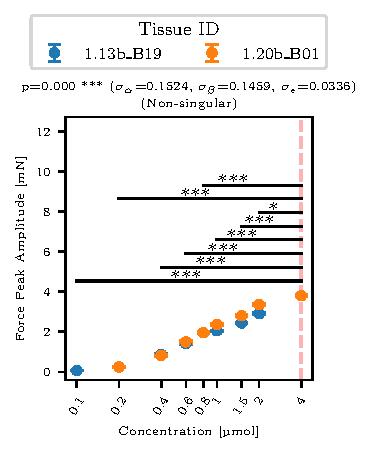
\includegraphics[width=\textwidth]{plots/chapter_5/ca_titration/significance_features_lmer_subset_1.pdf}
        %             \caption[Statistical Significance of Calcium Titration Experiment Across Biological Features.]{\textbf{}}
        %             \label{fig:sig_subset_ca_titration}
        %         \end{subfigure}
        %         ~
        %         \begin{subfigure}[b]{0.4\textwidth}
        %              \centering
        %             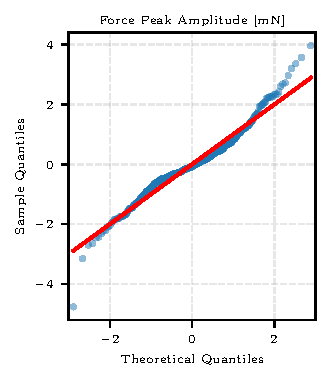
\includegraphics[width=\textwidth]{plots/chapter_5/ca_titration/qq_mixed_subset_1.pdf}
        %              \caption[]{}
        %              \label{fig:qq_subset_ca_titration}
        %         \end{subfigure}
        %         ~
        %         \begin{subfigure}[b]{0.5\textwidth}
        %              \centering
        %             \includegraphics[width=\textwidth]{plots/chapter_5/ca_titration/resid_anova_subset_1.pdf}
        %              \caption[]{}
        %              \label{fig:qq_subset_ca_titration}
        %         \end{subfigure}
        %         \caption[Statistical Significance of Calcium Titration with Diagnostic Plots]{ \textbf{Statistical Significance of Calcium Titration with Diagnostic Plots}: (a)
        %            Statistical Significance of Calcium Titration Experiment for Force Peak Amplitude (b) QQ Plot of Residuals for Mixed Model Fit of Calcium Titration Experiment. (c) Residuals vs. Fitted Values for Mixed Model Fit of Calcium Titration. }
        % \end{figure}
            % \begin{figure}
            %     \centering
            %     \includegraphics[width=1.0\textwidth, keepaspectratio]{plots/chapter_5/ca_titration/qq_mixed_subset_6.pdf}
            %     \caption[QQ Plot of Residuals for Mixed Model Fit of Calcium Titration Experiment]{\textbf{QQ Plot of Residuals for Mixed Model Fit of Calcium Titration Experiment.}}
            %     \label{fig:qq_subset_ca_titration}
            % \end{figure}
        
            % \begin{figure}
            %     \centering
            %     \includegraphics[width=1.0\textwidth, keepaspectratio]{plots/chapter_5/ca_titration/resid_mixed_subset_6.pdf}
            %     \caption[Residuals vs. Fitted Values for Mixed Model Fit of Calcium Titration.]{\textbf{Residuals vs. Fitted Values for Mixed Model Fit of Calcium Titration.}}
            %     \label{fig:fit_v_residual_subset_ca_titration}
            % \end{figure}
    \subsection{Section Summary}
       The statistical analysis confirms that the observed treatment effects align with expected physiological mechanisms, supporting the validity of the experimental approach. The results suggest that MTs exhibit pharmacological responses consistent with known treatment actions, making them a promising in vitro model candidates for studying cardiac treatment effects. However, further research is required to fully establish their translational relevance to human heart physiology, including comparing responses to human cardiac tissues and validating findings in additional experimental conditions.
        
\newpage
\section{Drug Response Modeling and Feature Analysis}
\label{sec:drug-response-feature-analysis}
  After assessing treatment effects, the next step was to identify biologically informative drug concentrations and analyze feature variations across treatments. This was achieved through the following steps:
    \begin{itemize}
        \item \textbf{Hill equation fitting} to model drug response curves and estimate the half-maximal effective concentration (\(\text{EC}_{50}\)) or inhibitory concentration (\(\text{IC}_{50}\)).
        \item \textbf{Relative comparison of treatment effects} by assessing changes in biological features at the \(\text{EC}_{50}\)/\(\text{IC}_{50}\) concentration in relation to baseline values.
        \item \textbf{Principal Component Influence Analysis (PCIA)} to systematically identify features that exhibit similar variation across different treatment concentrations, enabling a more data-driven understanding of treatment-induced effects.
    \end{itemize}

    The following sections provide a detailed explanation of each step.


    \subsection{Hill Fitting} 
    \label{sec:hillfitting}
        To model the dose-response relationship of the treatments, the Hill equation was fitted to the extracted features. The Hill equation is defined as:
        
        \begin{equation}
            \frac{E}{E_{\max}} = \frac{[A]^n}{\text{EC}_{50} + [A]^n}
        \end{equation}
        
        where:
        \begin{itemize}
            \item \(E\) represents the measured feature response.
            \item \(E_{\max}\) is the maximum observed feature response.
            \item \([A]\) is the treatment concentration.
            \item \(\text{EC}_{50}\) is the treatment concentration at which the response reaches half of \(E_{\max}\).
            \item \(n\) is the Hill coefficient, describing the steepness of the dose-response curve.
        \end{itemize}
        
        For this analysis, four key features were considered: \textit{Field Potential Duration (FPD)}, \textit{Force Peak Amplitude}, \textit{Calcium Peak Amplitude}, and \textit{Local Frequency}. The Hill equation was fitted to the data for Calcium Titration and Nifedipine, while E-4031 was excluded due to an insufficient number of concentration levels.
        
        Since the primary focus of this analysis was on overall treatment effects rather than inter-tissue variability, response values were averaged across tissues to ensure a generalized pharmacological interpretation.
        
        Hill fitting was performed using the \texttt{Hillfit} package \cite{himoto_hillfit} in Python (Figure~\ref{fig:hill_analysis}), and the estimated \(\text{EC}_{50}\)/\(\text{IC}_{50}\) values of above selected features were averaged and used for further analysis. The closest available experimental concentration available to this value was selected:
        \begin{itemize}
            \item \(\text{IC}_{50} \approx 1.22\) \SI{}{\umol} for Calcium Titration, mapped to the available concentration of \SI{1.0}{\umol}.
            \item \(\text{EC}_{50} \approx 0.91\) \SI{}{\umol} for Nifedipine, mapped to the available concentration of  \SI{1.0}{\umol}.
        \end{itemize}
        
        These values serve as a reference point for assessing the relative impact of pharmacological treatment in the next section.
        
        \begin{figure}[H]
            \centering
            \includegraphics[width=1.0\textwidth, height=0.8\textheight, keepaspectratio]{plots/chapter_6/ca_nifedipine_mean_hill_analysis_legend_fix.pdf}
            \caption[Hill Equation Fitting for Calcium Titration and Nifedipine.]{\textbf{Hill Equation Fitting for Calcium Titration Experiment and Nifedipine}:
            This figure presents the normalized dose-response curves for Calcium Titration (left) and Nifedipine (right), fitted using the Hill equation. Four key biological features were analyzed: \textit{Field Potential Duration (FPD) [\SI{}{\textit\s}]}, \textit{Force Peak Amplitude [\SI{}{\textit{\milli\newton}}]}, \textit{Ca$^{+2}$ Peak Amplitude [a.u]}, \textit{Local Frequency [\SI{}{\textit{\hertz}}]}. The Hill equation was used to estimate the half-maximal effective concentration (\(\text{EC}_{50}\)) and the inhibitory concentration (\(\text{IC}_{50}\)) for Calcium Titration experiment and Nifedipine, respectively. The fitted curves help quantify the non-linear drug response and allow comparison between experimental data and expected pharmacological behavior. The experimental concentration closest to the mean of estimated \(\text{EC}_{50}\)/\(\text{IC}_{50}\) values  (1.0 \SI{}{\umol}) was selected as a reference for subsequent analyses, ensuring that treatment-induced effects are evaluated at a biologically relevant dosage.}
        
            \label{fig:hill_analysis}
        \end{figure}
        
    \subsection{Relative Comparison of Treatment Effect}
    \label{sec:relative_comparison}

        To evaluate how pharmacological treatments modify biological features, responses at \(\text{EC}_{50}\)/\(\text{IC}_{50}\) were compared to baseline measurements. The baseline was defined by aggregating feature values across all conditions before treatment. 

        For each feature, the mean baseline value was set to 100\%, and the percent change at the selected \(\text{EC}_{50}\)/\(\text{IC}_{50}\) concentration was computed as:
        
        \begin{equation}
            \text{Relative Change (\%)} = \frac{\text{Feature Value at EC}_{50}-\text{Feature Value at Baseline}}{\text{Feature Value at Baseline}} \times 100
        \end{equation}
        
       By normalizing feature changes relative to baseline, this approach enables a direct and standardized comparison of drug effects across treatments, improving interpretability. The results are presented in Figure~\ref{fig:mean_relative_change_baseline_ec50}. For E-4031, where the mean \(\text{EC}_{50}\) could not be determined, the largest available concentration (0.003 \SI{}{\umol}) was used as a substitute.
        
        
        \begin{figure}[H]
            \centering
            \includegraphics[width=1\textwidth, keepaspectratio]{plots/chapter_6/ec_ic50_mean_relative_changes.pdf}
            \caption[Mean Relative Change of Features Across Treatments at \(\text{EC}_{50}\)/\(\text{IC}_{50}\)]{\textbf{Mean Relative Change of Features Across Treatments at \(\text{EC}_{50}\)/\(\text{IC}_{50}\)}:
            This figure compares the percentage change in biological features relative to baseline at treatment concentrations approximating \(\text{EC}_{50}\)/\(\text{IC}_{50}\) for Nifedipine and Calcium Titration (1.0 \SI{}{\umol}). The baseline is defined as the mean feature value before treatment, set at 100\%. The observed changes reflect the extent of treatment-induced modifications in cellular function. For E-4031, where \(\text{EC}_{50}\)/\(\text{IC}_{50}\) could not be determined, the highest available concentration (0.003 \SI{}{\umol}) was used as a reference. These relative comparisons facilitate cross-drug analysis by normalizing responses, enabling a clearer interpretation of each treatment’s impact on tissue function.}

            \label{fig:mean_relative_change_baseline_ec50}
        \end{figure}
        
   \subsection{Principal Components Influence Analysis (PCIA)}
    \label{sec:pcia}
        Beyond individual feature analysis, a systematic approach was developed to identify groups of features that respond similarly across different treatment concentrations. This helps in recognizing shared biological mechanisms and uncovering functionally related feature groups.

        
        The approach is based on \textbf{Principal Component Analysis (PCA)} to reduce data dimensionality while preserving variance and \textbf{DBSCAN clustering} of principal component (PC) loadings to group features with similar contribution patterns. More briefly, PCA was applied to each treatment data, and principal components explaining 95\% of the variance were retained (Figure \ref{fig:variance_explained_nifedipine}). Feature contributions (loadings) to these components were then extracted and clustered using DBSCAN. To determine the optimal \(\varepsilon\) parameter for DBSCAN, the k-nearest neighbors (\textit{k-NN}) heuristic was employed with \(k = 2\), ensuring that even a cluster with only two features having similar concentration-dependent variations could be identified. The knee point in the decreasingly sorted k-NN distance curve ($d_i$) was identified and used as \(\varepsilon\) value (Figure~\ref{fig:kneedle-curve}). The resulting clustered feature groups captured functionally related responses, while features categorized as noise points were identified as independently varying.
        
        To determine the optimal \(\varepsilon\) for DBSCAN, the Kneedle algorithm \cite{kneedle} was applied using the \texttt{Kneed} \cite{arvkevi_kneed} package in Python. Since the algorithm is designed for concavely increasing functions, it first inverts the k-nearest neighbors (k-NN) distance curve (${d_i}^{*}$) to adapt it for knee point detection. Before identifying the knee point, the algorithm normalizes both the sample indices (\(x\)-axis) and the corresponding k-distances (\(y\)-axis), ensuring a scale-independent detection of the knee region. Once the knee point is detected, the algorithm returns the corresponding unnormalized k-distance value, which is then used as the final \(\varepsilon\) parameter for DBSCAN. 
        

         \begin{figure}[H]
                \centering
                \begin{subfigure}[b]{0.4\textwidth}
                    \includegraphics[width=\textwidth, height=0.39\textheight]{plots/chapter_6/pfa_dbscan_explained_variance_nifedipine.pdf}
                    \caption[Variance Explained by Principal Component Analysis (PCA) for Nifedipine]{}
                    \label{fig:variance_explained_nifedipine}
                \end{subfigure}
                ~
                \begin{subfigure}[b]{0.4\textwidth}
                     \centering
                    \includegraphics[width=\textwidth]{plots/chapter_6/pfa_dbscan_kneedle_curve_nifedipine.pdf}
                    \caption[Kneedle Algorithm Fit for Determining DBSCAN Clustering Parameter (\(\varepsilon\)) in Nifedipine Analysis]{}
                    \label{fig:kneedle-curve}
                \end{subfigure}
                \caption[Variance Explained by PCA and Kneedle Fit]{\textbf{(a) Variance Explained by Principal Component Analysis (PCA) for Nifedipine}: 
                   Cumulative variance explained by principal components (PCs) derived from Nifedipine-treated samples. The red vertical line marks the retention of 8 components (out of 18 total) required to capture 95\% of the variance. These 8 PCs were used in subsequent clustering of feature loadings to group concentration-dependent responses. \textbf{(b) Kneedle Algorithm Fit for Determining DBSCAN Clustering Parameter in Nifedipine Analysis}: K-nearest neighbors (k-NN, k=2) distance curve ($d_i$) sorted in decreasing order is used to determine the optimal \(\varepsilon\) for DBSCAN clustering. The Kneedle algorithm inverts the distance curve for concavity-based detection. It then normalizes sample indices (x-axis) and distances (y-axis) to identify the knee point (black dotted line). The unnormalized distance (i.e. ${d_i}$) at this knee (0.2) was selected as \(\varepsilon\).
                   }
        \end{figure}
        
        The full procedure is summarized in Procedure~\ref{alg:pcia}.
        
        \begin{algorithm}[H]
        \caption{Principal Components Influence Analysis (PCIA)}
        \label{alg:pcia}
        \textbf{Input:} Treatment response data with features across concentrations \\
        \textbf{Output:} Feature clusters exhibiting similar variation and Independently varying features (Noise points)
        \begin{algorithmic}[1]
            \State Perform PCA on the treatment data and retain components explaining 95\% variance.
            \State Compute k-nearest neighbors distances for features with \( k = 2 \).
            \State Sort distances in decreasing order.
            \State Apply Kneedle algorithm to determine the knee point; take the unnormalized distance ($d_i$) at knee as \(\varepsilon\).
            \State Perform DBSCAN clustering using \(\varepsilon\) and min\_samples = 2 (minimum samples required to form a cluster).
            \State Return noise points and feature clusters.
        \end{algorithmic}
        \end{algorithm}
                
        Applying PCIA to \textit{Nifedipine} resulted in one major feature cluster, consisting of six features with similar PC loading contributions (Figure~\ref{fig:nifedipine_feature_cluster}). The similarity in their behavior was further confirmed by visualizing their relative change across different drug concentrations (Figure~\ref{fig:nifedipine-average-concentration-diffs}). 
        
        \begin{itemize}
            \item Most features exhibited a consistent trend across concentrations.
            \item One feature, \textit{Force Peak Amplitude}, was clustered with the other features but showed greater variation at higher concentrations in the relative change plot. This suggests that its response pattern deviates from the cluster assignment made by DBSCAN, potentially due to the heuristic-dependent parameters of the algorithm. Further refinement of the clustering approach, such as adjusting distance metrics, could improve feature grouping accuracy.
        \end{itemize}
        
        Overall, this methodology systematically identifies biologically meaningful feature clusters by grouping features with similarly varying responses across treatment concentrations. It reveals functional relationships between biological signals and provides a basis for generating hypotheses for further experimental validation, aiding in the understanding of treatment effects and their physiological implications.


        % \begin{figure}[H]
        %     \centering
        %     \includegraphics[width=0.5\textwidth, keepaspectratio]{plots/chapter_6/pfa_dbscan_explained_variance_nifedipine.pdf}
        %     \caption[Variance Explained by Principal Component Analysis (PCA) for Nifedipine]{\textbf{Variance Explained by Principal Component Analysis (PCA) for Nifedipine}: 
        %     This figure displays the cumulative variance explained by principal components (PCs) derived from Nifedipine-treated samples. The red vertical line highlights the number of components (8) required to retain 95\% of the variance.}
        %     \label{fig:variance_explained_nifedipine}
        % \end{figure}

        % \begin{figure}[H]
        %     \centering
        %     \includegraphics[width=0.5\textwidth, keepaspectratio]{plots/chapter_6/pfa_dbscan_kneedle_curve_nifedipine.pdf}
        %     \caption[Kneedle Algorithm Fit for Determining DBSCAN Clustering Parameter (\(\varepsilon\)) in Nifedipine Analysis]{\textbf{Kneedle Algorithm Fit for Determining DBSCAN Clustering Parameter (\(\varepsilon\)) in Nifedipine Analysis}: To optimize feature clustering based on principal component loadings, the \(\varepsilon\) parameter for DBSCAN was determined using the Kneedle algorithm. The plot shows the k-nearest neighbors (\textit{k-NN}) distance curve (K=2), with the knee point (black dotted line) identified as the optimal threshold for clustering (after de-normalizing). }
        %     \label{fig:kneedle-curve}
        % \end{figure}

       
        
        % \begin{figure}[H]
        %     \centering
        %     \includegraphics[width=0.99\textwidth, height=0.8\textheight,keepaspectratio]{plots/chapter_6/pfa_dbscan_cluster_report_nifedipine.pdf}
        %     \caption[Feature Clusters Derived from DBSCAN on Nifedipine Principal Component Loadings]{\textbf{Feature Clusters Derived from DBSCAN on Nifedipine Principal Component Loadings}: This figure shows the outcome of DBSCAN clustering applied to the loadings of principal components extracted from Nifedipine-treated samples. The identified clusters group features that exhibit similar variations across drug concentrations, suggesting shared underlying biological mechanisms.}
        %     \label{fig:nifedipine_feature_cluster}
        % \end{figure}

        % \begin{figure}[H]
        %     \centering
        %     \includegraphics[width=0.9\textwidth, keepaspectratio]{plots/chapter_6/relative_differences_nifedipine__average_only.pdf}
        %      \caption[Relative Change in Nifedipine-Induced Feature Modifications Across Drug Concentrations.]{\textbf{Relative Change in Nifedipine-Induced Feature Modifications Across Drug Concentrations}: This figure displays the relative changes in biological features under Nifedipine treatment, averaged across tissues. The trends illustrate how feature values progressively shift with increasing drug concentrations. Most features identified in a cluster (Force Peak Amplitude, Force Width 0.2, Force Width 0.5, Force Width 0.8, Force RT 0.2-0.8, Force DT 0.2-0.8) follow a consistent varying pattern across concentrations, confirming their functional grouping as identified by DBSCAN. However, the deviation observed in \textit{Force Peak Amplitude} at higher concentrations suggests that further refinement of clustering methods, such as alternative distance metrics, may improve clustering accuracy.}
        %     \label{fig:nifedipine-average-concentration-diffs}
        % \end{figure}
        % \newpage
        \begin{figure}[H]
                \centering
                \begin{subfigure}[b]{1\textwidth}
                    \includegraphics[height=0.3\textheight, keepaspectratio]{plots/chapter_6/pfa_dbscan_cluster_report_nifedipine.pdf}
                    \caption[Feature Clusters Derived from DBSCAN on Nifedipine Principal Component Loadings]{}
                    \label{fig:nifedipine_feature_cluster}
                \end{subfigure}
                
                \begin{subfigure}[b]{1\textwidth}
                     \centering                 
                    \includegraphics[height=0.54\textheight, keepaspectratio]{plots/chapter_6/relative_differences_nifedipine__average_only.pdf}
                     \caption[Relative Change in Nifedipine-Induced Feature Modifications Across Drug Concentrations.]{}
                     \label{fig:nifedipine-average-concentration-diffs}    
                \end{subfigure}
                \caption[Feature Clusters from PCIA and their Relative Change]{(a) \textbf{Feature Clusters Derived from DBSCAN on Nifedipine Principal Component Loadings}: This figure presents the DBSCAN clustering results applied to the principal component loadings of Nifedipine-treated samples. The heatmap visualizes the identified feature cluster (comprising six features) that exhibit similar loading contributions, highlighting their shared variation patterns across principal components. (b) \textbf{Relative Change in Nifedipine-Induced Feature Modifications Across Concentrations}: This figure displays the relative changes in biological features under Nifedipine treatment, averaged across tissues. The trends illustrate how feature values progressively shift with increasing drug concentrations. Most features identified in cluster from (a), namely \textit{Force Peak Amplitude, Force Width 0.2, Force Width 0.5, Force Width 0.8, Force RT 0.2-0.8, and Force DT 0.2-0.8} follow a consistent varying pattern across concentrations, confirming their functional grouping as identified by DBSCAN. However, the deviation observed in \textit{Force Peak Amplitude} at higher concentrations suggests that further refinement of clustering methods, such as alternative distance metrics, may improve clustering accuracy.}
            \end{figure}

        \subsection{Section Summary}
        This chapter presented a systematic approach to modeling drug responses and identifying biologically relevant feature variations at treatment-effective concentrations. Hill equation fitting successfully quantified drug potency, with estimated \(\text{EC}_{50}\)/\(\text{IC}_{50}\) values. The relative comparison framework enabled cross-treatment analysis by normalizing responses, while PCIA revealed feature clusters with shared variation patterns across treatment concentrations, providing insight into underlying biological mechanisms. These findings demonstrate the utility of quantitative modeling in drug effect analysis, supporting further experimental validation and refinement of in-vitro MT based cardiac models.
        
\newpage
\section{Correlation Trend Analysis}
    \label{correlation-trend}
    After establishing the dose-response relationships and assessing relative changes in features under pharmacological treatments in the previous chapter, this analysis focuses on investigating correlation patterns between feature pairs across different pharmacological conditions. The goal is to establish robust estimates of inter-feature relationships and observe how they align or deviate from baseline conditions. This can help identify biologically relevant feature associations that persist or shift under treatment influence.
    
    \subsection{Methodology}
    To analyze correlations that are consistent irrespective of tissues and concentrations of pharmacological experiment, bootstrapping was used to estimate the distribution of correlation coefficients between feature pairs under different pharmacological conditions and the baseline. Since the interest lies in identifying global correlation trends persisting under treatment exposure rather than tissue and concentration specific effects, the data from all baseline experiments and all pharmacological conditions were combined, giving rise to a distinct dataset for baseline and each pharmacological condition.
    
    From each dataset, \(N=1000\) bootstrap samples were generated, each containing half the size of the original dataset, with replacement. This approach distorts tissue-level and concentration-level effects, allowing for a more generalized view of correlation patterns under pharmacological influence. For each bootstrap sample, the \textbf{Spearman correlation coefficient} was computed for all feature pairs, and its distribution was estimated. The same procedure was repeated for each pharmacological condition as well as for the baseline condition.
    
    Spearman correlation was chosen due to its ability to capture non-linear relationships, which are often biologically relevant. The distribution of bootstrapped Spearman correlations for a subset feature pairs under baseline conditions, along with their kernel density estimations, is shown in Figure~\ref{fig:bootstrapped_spearman_correlation_subset_baseline_histogram}.

     \begin{figure}[H]
        \centering
        \includegraphics[width=1.0\textwidth, keepaspectratio]{plots/chapter_7/correlation_grid_baseline_histogram_optional_features_6.pdf}
        \caption[Bootstrapped Distribution of Spearman Correlations for subset of Feature Pairs Under Baseline Conditions]{\textbf{Bootstrapped Distribution of Spearman Correlations for subset of Feature Pairs Under Baseline Conditions}:  
        This figure presents the distribution of bootstrapped Spearman correlation coefficients for a subset of feature pairs in the baseline condition (N=1000). The kernel density estimation (KDE) curves overlaying the histograms provide a smooth representation of correlation distributions. The estimated mean($\mu$) and sigma($\sigma$) of bootstrapped correlation distribution for each feature pair are also shown.}
        \label{fig:bootstrapped_spearman_correlation_subset_baseline_histogram}
    \end{figure}
    
    \subsection{Results and Interpretation}
    To determine whether a correlation was significant, a 95\% confidence interval (CI) criterion was applied. The nature of correlation was classified based on the following conditions:
    \begin{itemize}
        \item \textbf{Positive correlation}: The 95\% confidence interval does not include zero, and all values within the interval are positive.
        \item \textbf{Negative correlation}: The 95\% confidence interval does not include zero, and all values within the interval are negative.
        \item \textbf{No significant correlation}: The 95\% confidence interval includes zero, indicating that the relationship is not statistically significant.
    \end{itemize}
    
    To compare correlation patterns across treatment conditions, a Venn diagram was generated to visualize the overlap of correlation classifications (positive, negative, or no correlation) across pharmacological conditions (Figure~\ref{fig:correlation_venn}). To specifically analyze treatment-induced effects, the Venn diagram focuses on how correlations persist or shift under different treatments, excluding baseline conditions. This helps differentiate between treatment-specific and shared biological interactions:
    \begin{itemize}
        \item \textbf{37} feature pairs exhibited the same correlation nature (either positive or negative) across all three conditions, suggesting that these relationships persist regardless of treatment.
        \item \ \textbf{E-4031} shared correlation patterns with \textbf{Nifedipine} for \textbf{4} feature pairs and with the \textbf{Calcium Titration experiment} for \textbf{9} feature pairs, respectively.
        \item \textbf{Nifedipine} and the \textbf{Calcium Titration experiment} exhibited \textbf{67} shared feature pair correlations, indicating that their effects on feature relationships are more similar to each other than to \textbf{E-4031}.
        \item Unique correlation patterns were observed for \textbf{1, 14}, and \textbf{16} feature pairs under \textbf{E-4031, Nifedipine}, and the \textbf{Calcium Titration experiment}, respectively, suggesting that these pharmacological stimuli induce distinct interactions between certain features.
    \end{itemize}

    \begin{figure}[H]
        \centering
        \includegraphics[width=0.5\textwidth, keepaspectratio]{plots/chapter_7/correlation_venn.pdf}
         \caption[Venn Diagram of Shared Correlation Patterns Across Treatments]{\textbf{Venn Diagram of Shared Correlation Patterns Across Treatments}:
            This figure illustrates the overlap in correlation classifications (positive, negative, or non-significant) among the three pharmacological treatments: E-4031, Nifedipine, and Calcium (Ca\textsuperscript{2+}) Titration. 
            A total of 37 feature pairs exhibit consistent correlations across all three treatments, suggesting stable biological associations. Nifedipine and Calcium Titration share 67 feature pair correlations, indicating a stronger similarity in their effects. In contrast, E-4031 shares only 4 correlations with Nifedipine and 9 with the Calcium Titration experiment. Unique correlation patterns are observed for 1, 14, and 16 feature pairs under E-4031, Nifedipine, and Calcium Titration, respectively, highlighting treatment-specific effects on feature relationships.}
        \label{fig:correlation_venn}
    \end{figure}

    
    Since the baseline condition was not included in the Venn diagram, a separate visualization was developed to compare treatment-induced correlation trends to baseline. More briefly, a trend comparison was visualized in a line plot (Figure~\ref{fig:line_plot_correlation_trend}). In this plot:
    \begin{itemize}
        \item The x-axis represents feature pairs (mapped to a unique id).
        \item The y-axis shows the bootstrapped mean of Spearman correlation coefficients for each feature pair, along with the shaded 95\% confidence interval.
    \end{itemize}
    Feature pairs were sorted based on their baseline correlation, with strongly positive correlations on the left side of the plot transitioning toward negative correlations on the right. Due to the large number of feature pairs and for visualization clarity, each feature pair on the x-axis is mapped to a unique identifier instead of displaying full feature names. The dictionary defining the mapping between feature pairs and their corresponding IDs is provided in the supplementary section (Section \ref{feature-mapping}).
    
    This visualization provides a high-level, bird's-eye view of how different treatments alter biological interactions. It captures general trends in feature associations, offering insights into potential drug and treatment mechanisms and side effects. However, due to the large number of feature pairs, detailed interpretation requires zooming in on specific associations.
    
    A key consideration in interpreting the results is the degree of overlap in confidence intervals. Many confidence intervals, particularly those around zero (seen in the right portion of the plot for baseline), suggest that the correlation is not statistically significant. Therefore, only feature pairs where the confidence interval does not include zero should be considered for further investigation.

    
    \textbf{Example Interpretation:} For instance, the correlation between \textit{Duration} and \textit{Force Peak Amplitude} shows a significant positive correlation under baseline conditions, which is retained under Nifedipine and E-4031 but not in the Calcium Titration experiment, where the mean correlation shifts toward negative values. This suggests that the relationship between \textit{Duration} and \textit{Force Peak Amplitude} remains stable under Nifedipine and E-4031, but is altered by Calcium Titration, possibly due to calcium availability significance in ECC (Figure \ref{fig:line_plot_correlation_trend}).
    \begin{figure}[H]
        \centering
        \includegraphics[width=1\textwidth, keepaspectratio, height=1.0\textheight]{plots/chapter_7/drug_correlations_comparison_numbered_annotated.pdf}
        \caption[Treatment-Induced Changes in Feature Pair Correlation Trends Compared to Baseline]{\textbf{Treatment-Induced Changes in Feature Pair Correlation Trends Compared to Baseline}:
            This figure visualizes the mean of bootstrapped distribution of Spearman correlation coefficients for \textbf{153 feature pairs} across baseline and treatment conditions. The x-axis represents feature pairs, each mapped to a unique identifier for visualization clarity instead of displaying full feature names (Section~\ref{feature-mapping}). Feature pairs are sorted from \textbf{strong positive correlations} (left) to \textbf{strong negative correlations} (right) based on baseline correlation. The y-axis shows the mean correlation values, with shaded regions indicating \textbf{95\% confidence intervals}. Feature pairs with confidence intervals overlapping zero indicate weak or non-significant correlations. \textbf{Example Interpretation (Middle Box):} The correlation between \textit{Duration} and \textit{Force Peak Amplitude} is significantly positive under baseline conditions and remains stable under Nifedipine and E-4031. However, in Calcium Titration, the mean correlation shifts toward negative values, suggesting a disruption in their relationship.}
        
        \label{fig:line_plot_correlation_trend}
    \end{figure}

    Such a correlation trend can be used to identify feature pair associations that differ or persist across drug and treatment conditions. Additionally, some correlations may strengthen or weaken under treatment conditions compared to baseline, providing insights into treatment-induced interactions.


    
    \subsection{Biological Implications and Summary}
    This analysis provides a high-level, bird's-eye view of how pharmacological treatments influence biological feature associations by examining global correlation patterns across treatments. Bootstrapped Spearman correlations were used to identify both stable biological relationships and treatment-specific shifts, offering initial insights into potential modifications in biological pathways. Feature pairs that maintain consistent correlations across all conditions may represent fundamental biological interactions, whereas treatment-specific changes could indicate distinct pharmacological effects or potential side effects due to cross-treatment interactions.
    
    It is important to emphasize that these findings represent broad statistical associations rather than mechanistic causal relationships among feature pairs. As an initial screening tool, this analysis helps characterize treatment effects at a systems level, guiding future studies toward more targeted experimental validation or predictive modeling to explore specific biological mechanisms in greater depth.
    
\newpage
\section {Modeling Treatment-Induced Feature Associations} 
\label{regression-feature-associations}
    Following the exploration of global correlation trends among feature pairs, the final phase of the analysis focuses on identifying statistical associations between individual features under both baseline and pharmacological/experimental conditions through multiple regression. While this analysis does not provide a mechanistic explanation of tissue dynamics, it establishes an essential statistical framework for identifying potential regulatory interactions. This framework serves as a starting point for further modeling and experimental validation of treatment effects on MTs.

    To quantify these associations, a mixed modeling approach with \textbf{LASSO regression} was applied, where each feature was considered as the target variable and regressed against all other features. This was performed across both baseline and three experimental conditions of this study, allowing for the identification of statistical relationships that persist or change in response to pharmacological stimuli.

    \subsection{Model Specification}
    As in previous analyses, data across different treatment concentrations and tissues were merged to study the overall effect. However, as discussed in significance analysis (Section~\ref{chap:statistical_analysis}), some tissues lacked data points for certain concentrations (Tables~\ref{tab:nifedipine} and \ref{tab:ca_titration}), creating an unbalanced repeated-measures design. This was addressed using an appropriately nested mixed-effects model. However, in the current analysis, where each feature is regressed over all remaining features, the high-dimensional nature of the dataset necessitated the use of \textbf{LASSO regularization} to shrink coefficients of non-contributory predictors.
        
    Due to current limitations in applying LASSO to mixed models, only the \texttt{glmmLASSO} \cite{Schelldorfer03042014} package was available, which does not support a fully nested structure. To accommodate this, concentrations with missing data for one or more tissues were removed, converting the dataset into a crossed design. The final mixed model incorporated \textbf{tissue} and \textbf{concentration} as \textbf{random effects} with an intercept, while all other features were included as \textbf{fixed effects}. The general model structure is given by:
    
       \[
        x_j = \beta_0 + \sum_{i \neq j} \beta_i x_i + Z_\alpha \cdot \text{[Tissue ID]} + Z_\beta \cdot \text{[Concentration]} + \epsilon
        \]
        
        where:
        \begin{itemize}
            \item \( x_j \) is the target feature, analogous to \( Y \) in the statistical significance model~\ref{e4031-met}.
            \item \( \beta_0 \) is the intercept, capturing the overall mean response.
            \item \( x_i \) represents all other features (\( i \neq j \)) included as fixed effect covariates with coefficients $\beta_i$, extending the previous model by incorporating additional predictors.
            \item \( Z_\alpha \) is the random intercept for \textbf{tissue}, modeled as \( Z_\alpha \sim \mathcal{N}(0, \sigma_\alpha^2) \), consistent with the statistical significance model.
            \item \( Z_\beta \) is the random intercept for \textbf{concentration}, modeled as \( Z_\beta \sim \mathcal{N}(0, \sigma_\beta^2) \), thereby transitioning concentration from a fixed effect to a random effect in this model.
            \item \( \epsilon \sim \mathcal{N}(0, \sigma^2) \) represents the residual error.
        \end{itemize}
        This formulation assumes that the random effects of tissue and concentration are uncorrelated. However, in a more generalized setting, a full covariance structure\footnote{Mixed models allow for the specification of covariance structures between random effects, such as an \textbf{unstructured} or \textbf{compound symmetry} covariance matrix. These structures model dependencies between random effects rather than assuming independence. For further details, see \cite{PinheiroBates2000}} could be used to model potential correlations between these random effects.
        
    For each regression, the optimal LASSO shrinkage parameter (\( \lambda \)) was determined through \textbf{5-fold cross-validation}, selecting the value that minimized residual deviance. Baseline conditions from all experiments were combined to serve as a reference.
    
    \subsection{Results and Interpretation}
    
    The results of the regression analysis are visualized in Figure~\ref{fig:regression}, where instead of displaying numerical coefficient values, a color-coded heatmap representation is used to facilitate comparison between baseline and treatment-induced conditions. Each regression’s optimal five-fold cross-validated \( \lambda \) value is also provided.
    
    As highlighted earlier, this analysis is not intended to serve as a definitive mechanistic model but rather as a \textbf{high-level exploratory framework} for identifying statistical associations among multiple features that may guide further investigations. Some consistent coefficient patterns are observable across both treatment and baseline conditions, particularly in the bottom right of Figure~\ref{fig:regression}, where strong statistical associations persist regardless of pharmacological intervention. The observed differences in regression coefficients across treatment conditions may provide valuable insights into how specific features interact under varying pharmacological influences.

    \begin{figure}
        \centering
        \includegraphics[width=1\textwidth, keepaspectratio]{plots/chapter_8/coefficient_heatmap_pair.pdf}
        \caption[Feature Associations Identified via Generalized Linear Mixed Model with LASSO Regularization (Baseline \& Nifedipine)]{\textbf{Feature Associations Identified via Generalized Linear Mixed Model with LASSO Regularization (Baseline \& Nifedipine)}:
            The heatmaps visualizes the regression coefficients obtained from the LASSO-regularized generalized linear mixed model (GLMM-LASSO) applied to the dataset under baseline and  Nifedipine drug. The analysis identifies statistical associations between features while accounting for inter-tissue and concentration-level variability. Each cell represents the magnitude and direction of the estimated coefficient for a given feature pair, with a color gradient indicating positive or negative associations. The LASSO shrinkage parameter (\(\lambda\)) was selected using 5-fold cross-validation, ensuring optimal coefficient regularization while minimizing residual deviance. Persistent feature relationships across both baseline and drug condition (observed in the lower right region of the heatmap) suggest stable biological interactions, while changes in coefficient patterns under drug treatments indicate pharmacologically induced modifications in feature associations. This model serves as an exploratory framework for identifying key regulatory interactions that may guide further experimental validation and mechanistic modeling of treatment-induced effects in MTs. The heatmaps for E-4031 and Calcium Titration are provided in supplementary figure (Figure \ref{fig:regression-sup})}
        \label{fig:regression}
    \end{figure}
    
    % \section{Biological Implications and Future Directions}
    
    % This methodology provides an initial statistical foundation for understanding the regulatory interactions governing cardiac contraction dynamics in MTs. While statistical associations do not imply causality, they highlight features that may warrant further biological investigation. The differences in feature associations between baseline and treatment-induced conditions suggest potential shifts in regulatory mechanisms that could be explored through mechanistic modeling or experimental validation.

    % Future studies could refine this approach by incorporating Bayesian shrinkage methods, which allow the integration of biological priors into the regression framework. Additionally, dynamic modeling techniques that capture time-dependent responses may offer deeper insights into treatment-induced tissue dynamics, ultimately contributing to more predictive models of MTs behavior.

    \subsection{Biological Implications and Summary}
    This chapter applied LASSO-regularized based mixed modeling regression to identify statistical associations between biological features under baseline and pharmacological/experimental conditions. By regressing each feature against all others while accounting for tissue and concentration variability, the analysis revealed both persistent feature interactions and condition-specific shifts in association patterns. While these results do not imply causality, they offer a high-level statistical framework to guide future investigations into regulatory changes induced by pharmacological stimulus.
    
% \chapter{Integrative Discussion and Conclusion}

% This thesis developed and validated an integrative methodology for the characterization of treatment-induced responses in myocardial tissues (MTs) derived from human-induced pluripotent stem cells (hiPSCs), specifically focusing on excitation-contraction coupling (ECC) dynamics. The comprehensive pipeline established in this study comprised preprocessing for signal noise reduction, biologically relevant feature extraction, sophisticated data mining, and robust statistical analyses. Detailed preprocessing methods, including noise filtering and contraction event identification, laid the foundation for accurate downstream analysis (Chapter \ref{data-prep}). Subsequently, advanced analytical methods, including feature space visualization via t-SNE, statistical modeling, drug-response modeling, principal component-based feature grouping, correlation trend analysis, and regression-based feature associations, were systematically employed to uncover biologically relevant insights (Chapter \ref{analysis}).

%     \section{Summary of Methodology, Results, and Evaluation}
%     The preprocessing pipeline effectively reduced signal noise through low-pass filtering, discrete wavelet transform (DWT)-based denoising, and baseline correction methods, thereby enhancing the robustness of subsequent analyses (Section \ref{signal-enhancement}). Notably, contraction event identification leveraged a prominence-based peak detection algorithm, though occasional inaccuracies were observed in low signal-to-noise conditions, highlighting a limitation that could be addressed with adaptive methods sensitive to varying signal-to-noise ratios (Section \ref{contraction-events}). The classification and removal of arrhythmic contractions were successful, ensuring only physiologically valid contraction events were analyzed (Section \ref{sec:arrythmia}).
    
%     Feature extraction methods provided robust quantification of critical ECC parameters across multiple signal modalities (force, calcium, and field potential), forming the foundation for subsequent analyses (Section \ref{feature-extraction}). The data mining approaches applied subsequently, including t-SNE visualization, offered a global view of treatment-induced effects and revealed overlapping feature distributions belonging to different pharmacological treatments, albeit with inherent limitations regarding interpretability due to non-linear projection (Section \ref{global-overview}).
    
%     Statistical analyses involving mixed modeling provided precise evaluations of treatment-induced feature effects, confirming expected physiological outcomes consistent with the existing literature (Sections \ref{e4031-significance-analysis}–\ref{ca-significance-analysis}). Drug-response modeling using the Hill equation yielded biologically meaningful \(\text{EC}_{50}\)/\(\text{IC}_{50}\) values; however, limited data points at intermediate concentrations highlighted a significant limitation in accurately modeling dose-response curves (Section \ref{sec:hillfitting}). Principal Component Influence Analysis (PCIA)  facilitated grouping of similarly varying features, though dependence on heuristically determined clustering parameters remains a limitation, suggesting exploration of alternative clustering methods in future studies (Section \ref{sec:pcia}).
    
%     Bootstrapping based correlation trend analysis effectively identified stable feature associations under varying pharmacological conditions, offering preliminary insights into ECC dynamics rather than causal relationships (Section \ref{correlation-trend}). Regression-based feature association using LASSO-regularized mixed models highlighted key feature interdependencies, yet the absence of nesting tissue effects under concentration levels presented a limitation, pointing to potential enhancements via methods capable of addressing nested experimental designs (Section \ref{regression-feature-associations}).
    
%     \section{Limitations and Future Directions}
%     The established methodology, while robust, presents several limitations, including occasional inaccuracies in baseline correction for calcium signals with sloped baselines and challenges in accurate Hill equation fitting due to sparse experimental data points. Future improvements could include adaptive baseline correction techniques, increased concentration resolution for drug-response modeling, exploration of more robust clustering techniques for PCIA, and implementation of nested regression models or non-linear analytical frameworks like decision trees and Bayesian approaches.
    
%     \section{Biological Implications}
%     Biologically, this study emphasizes the utility of MTs in modeling human cardiac drug responses, highlighting their potential for preclinical drug screening. Findings demonstrate clear tissue-specific responses to pharmacological perturbations, reinforcing the biological validity of MTs as predictive human cardiac models. The methodology not only facilitates deeper understanding of drug-induced modulation of ECC dynamics but also has significant implications for developing targeted cardiac therapies, improving the precision and relevance of preclinical screenings.
    
%     \section{Future Directions}
%     Future research could leverage the presented methodology to explore additional pharmacological stimulus, expand the range of analyzed ECC features, and integrate multi-tissue data to strengthen generalizability and predictive power. Furthermore, incorporating molecular-level insights through multi-omics analyses could complement current empirical observations, bridging molecular mechanisms with physiological responses.
    
%     \section{Conclusion}
%     In conclusion, the systematic approach presented in this thesis successfully integrates advanced signal processing and statistical methods to characterize pharmacological influences on ECC dynamics in MTs. By bridging empirical data with biological interpretation, this study contributes significantly toward the validation of hiPSC-derived myocardial tissues as reliable, human-relevant cardiac models for drug testing, ultimately aiding in the advancement of cardiac pharmacology and therapeutic development.

\chapter{Integrative Discussion and Conclusion}

    \section{Integrative Summary of Thesis Work}
    This thesis develops a comprehensive, data-driven pipeline to characterize how different pharmacological interventions modulate ECC in iPSC-derived MTs. The motivation stems from limitations in existing approaches, which often consider ECC parameters independently without accounting for their interrelationships or variability due to experimental conditions. To address these gaps, the thesis integrates multimodal data—contractile force, calcium transients, and field potentials—under interventions with E-4031, Nifedipine, and Calcium Titration.

    The analytical workflow begins with meticulous preprocessing designed to improve signal fidelity. Signal noise was reduced using Butterworth and Savitzky-Golay filters for force and calcium signals, and discrete wavelet transform-based denoising for field potentials. Baseline offsets due to sensor drift were corrected using Gaussian-based histogram fitting methods, ensuring accurate signal representations. Subsequently, peak-detection algorithms identified contraction events, which were further filtered to exclude arrhythmic contractions using machine learning classifiers.
    
    Following preprocessing, biomarkers quantifying the ECC cycle—such as peak amplitudes, contraction and relaxation times, and field potential durations—were systematically extracted and fed into a suite of analytical methods. Initially, a global overview was obtained using t-SNE visualization to detect inherent patterns and potential clustering across treatments and concentration levels, providing immediate insights into data structure and treatment similarity.
    
    Statistical significance was assessed through mixed-effects modeling, accounting explicitly for tissue-to-tissue and tissue-to-concentration variability, confirming known pharmacological effects. Dose–response (Hill) modeling further characterized the relative impact of treatments, establishing the potency and effect magnitude for each treatment compared to baseline conditions. Principal Components Influence Analysis (PCIA) was developed to identify groups of features responding similarly across treatment concentrations, revealing clusters indicative of jointly modulated biological processes. 
    
    Subsequent correlation analysis established global feature correlation trends, identifying both conserved interactions suggestive of shared pathways and novel, treatment-specific correlations indicative of treatment-specific effects. Finally, LASSO-regularized regression modeling evaluated how each individual feature was influenced by other features, providing foundational information necessary for future mechanistic modeling and deeper insights into feature interplay under pharmacological influence. A concise summary of the applied methods and their outcomes is provided in Table \ref{tab:methods-summary}.
    
    The combined outcomes validated known mechanisms, such as E-4031 prolonging repolarization and Nifedipine reducing contraction force, while also uncovering novel feature interactions that inform future research into ECC modulation. Collectively, this thesis provides a framework for future researchers aiming to understand and characterize pharmacological effects of different treatments on ECC modulation of MTs.

    \begin{table}[htbp]
    \centering
    \caption{Summary of Methodologies and Outcomes}
    \label{tab:methods-summary}
    \renewcommand{\arraystretch}{1.4}
    \begin{tabularx}{\textwidth}{@{}>{\raggedright}p{3.5cm}>{\raggedright}p{4.8cm}>{\raggedright}p{3.9cm}c@{}}
        \toprule
        \textbf{Method Step} & \textbf{Techniques Applied} & \textbf{Outcome} & \textbf{Section} \\
        \midrule \addlinespace[5pt]
        
        Signal Preprocessing & Butterworth filtering, Savitzky-Golay smoothing, DWT denoising & 
        Enhanced signal quality across modalities & \ref{signal-enhancement} \\ \addlinespace[5pt]
        
        Peak Detection & Prominence thresholding, Gaussian Mixture Models & 
        Robust contraction event detection & \ref{contraction-events} \\ \addlinespace[5pt]
        
        Arrhythmia Detection & Machine learning classification (Random Forest) & 
        High-fidelity arrhythmia exclusion & \ref{sec:arrythmia} \\ \addlinespace[5pt]
        
        Feature Extraction & Peak characterization, Duration measurements & 
        Comprehensive biomarker extraction & \ref{feature-extraction} \\ \addlinespace[5pt]
        
        Global Visualization & t-SNE dimensionality reduction & 
        Global overview of feature space and potential identification of clusters & \ref{global-overview} \\ \addlinespace[5pt]
        
        Statistical Testing & Mixed-effects modeling & 
        Establishment of significant treatment effects on biomarkers & \ref{chap:statistical_analysis} \\ \addlinespace[5pt]
        
        Dose-response \& Relative Feature Analysis & Hill equation modeling & 
        Quantitative treatment effect estimation against baseline & \ref{sec:hillfitting}--\ref{sec:relative_comparison} \\ \addlinespace[5pt]
        
        PCIA & PCA with DBSCAN clustering & 
        Identification of co-varying biomarkers & \ref{sec:pcia} \\ \addlinespace[5pt]
        
        Correlation Analysis & Bootstrapped correlation analysis & 
        Discovery of treatment-resistant and treatment-specific associations & \ref{correlation-trend} \\ \addlinespace[5pt]
        
        Regression Modeling & Regularized (LASSO) mixed-effects regression & 
        Establishment of foundational information for mechanistic modeling & \ref{regression-feature-associations} \\ \addlinespace[5pt]
        
        \bottomrule
    \end{tabularx}
\end{table}



    
    \section{Discussion on Methodology}
    
    \subsection{Preprocessing and Signal Enhancement}
   The preprocessing approach encompassed noise reduction through low-pass filtering for force and calcium signals, and Discrete Wavelet Transform (DWT) based denoising for field potential (FP) signals (Section~\ref{signal-enhancement}). While effective, the empirical determination of wavelet threshold values and baseline correction parameters can introduce biases—particularly if denoising inadvertently delays signal peaks or attenuates amplitudes, which may significantly affect subsequent analyses. Future studies could explore automated, data-driven methods for selecting optimal denoising thresholds to enhance robustness and reliability.

    Peak detection for contraction-event identification relied on prominence-based algorithms, demonstrating effectiveness under most conditions (Section~\ref{contraction-events}). However, the thresholds chosen here may not generalize well to datasets with different noise characteristics, and inaccurate thresholds can bias results by either missing real peaks or including noise spikes. Developing more adaptive or data-driven thresholding methods remains a critical avenue for improvement, especially for low signal-to-noise ratio scenarios.
    
    
    
    \subsection{Feature Visualization and Statistical Significance}
    Feature space visualization using t-SNE provided valuable insights into global data structure, highlighting overlapping pharmacological effects and distinct tissue-specific responses (Section \ref{global-overview}). Nevertheless, the inherent limitation of t-SNE—its inability to accurately preserve original data distances—restricts quantitative interpretation, suggests linear dimensionality reduction techniques might provide complementary insights.
    
    Statistical significance testing via mixed-effects modeling effectively handled repeated measures and nested treatment designs, confirming drug-induced physiological effects consistent with literature (Sections \ref{e4031-significance-analysis}–\ref{ca-significance-analysis}). Given only two tissue replicates, simpler statistical methods like ANOVA could have sufficed, but the chosen mixed modeling approach is justified due to its scalability for future larger studies involving multiple tissues.
    
    \subsection{Drug Response Modeling and Limitations}
    The application of Hill equation modeling facilitated quantitative drug response characterization, providing an estimate of \(\text{EC}_{50}\)/\(\text{IC}_{50}\) values for the studied pharmacological stimulus (Section \ref{sec:hillfitting}). However, limited concentration points restricted model accuracy. The substantial gaps between tested concentrations impeded precise curve-fitting, highlighting a clear need for increased data points at intermediate concentrations for improved curve fitting and reliable pharmacological characterization in future work.
    
    Grouping of  features using Principal Component Influence Analysis (PCIA) through DBSCAN clustering effectively identified feature clusters which followed similar variation patterns across different concentrations of a treatment, demonstrating consistent pharmacological modulation (Section \ref{sec:pcia}). Yet, heuristic parameter selection for DBSCAN is a clear limitation. Future research should implement more robust, parameter-agnostic clustering algorithms to enhance reproducibility and accuracy.
    
    \subsection{Feature Associations and Correlation Analysis}
    Correlation trend analysis, involving bootstrapped correlation distributions across treatments, effectively captured global feature relationships, highlighting persistent and unique feature pair associations (Section \ref{correlation-trend}). However, these correlation analyses only suggest statistical relationships, not causal interactions, and should be regarded as exploratory rather than definitive. Additional experiments or mechanistic studies would be needed to ascertain causal pathways.
    
    The regression-based association study using mixed-model LASSO regression provided a useful preliminary tool for identifying inter-feature relationships while controlling for experimental variability (Section \ref{regression-feature-associations}). A key limitation was the inability of this approach to explicitly model nested structures (concentration within tissue). More sophisticated approaches, such as Bayesian hierarchical modeling for incorporating biological feature priors or non-linear interpretable methods like decision trees, could be explored in future studies to better capture biological complexity.
    
    \paragraph{}
    A further overarching limitation of this research is its reliance on only two tissue replicates for pharmacological testing. While sufficient for a proof of concept, larger sample sizes and additional tissues would provide stronger statistical power and broader generalizability of findings. Integrating more tissue replicates, increased concentration sampling, and parameter-agnostic algorithms in future work will enhance the robustness, reproducibility, and practical impact of these methodological advances.

    \section{Biological Implications}
    This thesis bridges a key gap established in the literature (Chapter \ref{literature}) by integrating multimodal data (electrical, calcium, and mechanical) with robust statistical modeling to explore both individual biomarker changes and cross-biomarker relationships in ECC. Whereas many prior studies focused on isolated endpoints, the approach here systematically correlates multiple ECC parameters, revealing both conserved interactions (indicating fundamental physiological processes) and treatment-specific alterations (highlighting treatment-related mechanisms). By explicitly accounting for tissue-level variability through mixed-effects modeling, the framework advances beyond standard methods that often overlook inter-tissue differences. Overall, combining signal processing, correlation analyses, dose–response estimation, and regression in a unified pipeline demonstrates how high-content, multimodal data can yield deeper biological insights than conventional single-parameter approaches in ECC pharmacodynamics.
    
    \section{Future Research Directions}
    Although this pipeline effectively characterizes and interprets treatment-induced changes in ECC, several avenues remain for further enhancement. First, while arrhythmic events were excluded in this study, future work could incorporate arrhythmic events, potentially enhancing predictions of pro-arrhythmic risk. Second, applying the same analysis framework to other muscle tissue types—with appropriate parameter tuning for denoising and peak detection—would broaden its relevance beyond cardiac contexts. Third, increasing the number of tissue replicates and sampling finer concentration gradients would strengthen statistical power, refine dose–response modeling, and better capture biological variability. Finally, exploring more advanced or non-linear modeling strategies, such as hierarchical Bayesian and Tree-based approaches, could uncover additional biomarker interdependencies and help unify empirical data with mechanistic models of cardiac physiology.
    
    \section{Conclusion}
    This thesis developed a robust, data-driven analytical framework to systematically characterize how pharmacological interventions modulate ECC in hiPSC-derived MTs. Despite certain methodological constraints—such as empirical threshold settings, limited tissue replicates, and inadequate concentration sampling—the proposed approach effectively captured physiologically relevant treatment responses. By combining advanced signal preprocessing, peak detection, arrhythmia classification, and feature extraction with rigorous statistical learning–based modeling, the pipeline reliably characterized treatment-induced physiological responses.

    While heuristic-dependent parameters in signal preprocessing and feature extraction present clear avenues for refinement, the integrative methodology nonetheless revealed treatment-specific and conserved patterns indicative of pharmacological modulation. These insights reinforce the growing utility of multimodal MTs in human cardiac pharmacology, underscoring the potential for improved preclinical screening. 
    
    Moving forward, future work should address current limitations by expanding the dataset, refining signal processing and arrhythmia detection, and exploring more sophisticated modeling strategies (e.g., decision trees). Such endeavors would further enhance the scalability and translational value of MT-based assays, laying the groundwork for more precise preclinical predictions in cardiac drug development.
    
    

% \chapter*{References}  % References (Unnumbered)
\printbibliography

\addcontentsline{toc}{chapter}{References}  % Add to TOC

\appendix  % Start supplementary material section

\chapter{Supplementary Material}  % Supplementary Material as a numbered chapter

    \section{Significance Analysis}
            The significance plots and diagnostic plots for E-4031 (Figures \ref{fig:e4031-remaining-significance}, \ref{fig:e4031-remaining-qq}, \ref{fig:e4031-remaining-resid}) and Nifedipine (Figures \ref{fig:nifedipine-remaining-significance}, \ref{fig:nifedipine-remaining-qq} and \ref{fig:nifedipine-remaining-resid}) are presented below.
        
        
    \begin{figure}
        \centering
        \includegraphics[width=1\textwidth, height=0.99\textheight, keepaspectratio]{plots/chapter_5/e4031/significance_features_lmer_subset_15.pdf}
        \caption[Statistical significance of E-4031 treatment on remaining Biological features.]{\textbf{Statistical significance of E-4031 treatment on remaining Biological features.}.}
        \label{fig:e4031-remaining-significance}
    \end{figure}

    \begin{figure}
        \centering
        \includegraphics[width=1\textwidth, height=0.99\textheight, keepaspectratio]{plots/chapter_5/e4031/qq_mixed_subset_15.pdf}
        \caption[QQ Plot of Residuals for Mixed Model Fit of E-4031 Treatment (Remaining Features)]{\textbf{QQ Plot of Residuals for Mixed Model Fit of E-4031 Treatment (Remaining Features)}}
        \label{fig:e4031-remaining-qq}
    \end{figure}

    \begin{figure}
        \centering
        \includegraphics[width=1\textwidth,height=0.99\textheight, keepaspectratio]{plots/chapter_5/e4031/resid_mixed_subset_15.pdf}
        \caption[Residuals vs. Fitted Values for Mixed Model Fit of E-4031 Treatment (Remaining Features)]{\textbf{Residuals vs. Fitted Values for Mixed Model Fit of E-4031 Treatment (Remaining Features).}}
        \label{fig:e4031-remaining-resid}
    \end{figure}

    \begin{figure}
        \centering
        \includegraphics[width=1\textwidth, height=0.99\textheight, keepaspectratio]{plots/chapter_5/nifedipine/significance_features_lmer_subset_12.pdf}
        \caption[Statistical significance of Nifedipine treatment on remaining Biological features.]{\textbf{Statistical significance of Nifedipine treatment on remaining Biological features.}.}
        \label{fig:nifedipine-remaining-significance}
    \end{figure}

    \begin{figure}[H]
        \centering
        \includegraphics[width=0.8\textwidth, keepaspectratio]{plots/chapter_5/nifedipine/qq_mixed_subset_12.pdf}
        \caption[QQ Plot of Residuals for Mixed Model Fit of Nifedipine Treatment (Remaining Features)]{\textbf{QQ Plot of Residuals for Mixed Model Fit of Nifedipine Treatment (Remaining Features)}}
        \label{fig:nifedipine-remaining-qq}
    \end{figure}

    \begin{figure}[H]
        \centering
        \includegraphics[width=0.8\textwidth, keepaspectratio]{plots/chapter_5/nifedipine/resid_mixed_subset_12.pdf}
        \caption[Residuals vs. Fitted Values for Mixed Model Fit of Nifedipine Treatment (Remaining Features)]{\textbf{Residuals vs. Fitted Values for Mixed Model Fit of Nifedipine Treatment (Remaining Features).}}
        \label{fig:nifedipine-remaining-resid}
    \end{figure}

    \section{Feature Associations via LASSO based Mixed Modeling}
    \label{feature-association-e4031-ca}

    This section contains the LASSO based Mixed modeling regressions plots (Section \ref{regression-feature-associations}) for E-4031 and Calcium Titration experiment. (Figure \ref{fig:regression-sup})

     \begin{figure}
        \centering
        \includegraphics[width=1\textwidth, keepaspectratio]{plots/chapter_8/coefficient_heatmap_pair_supplementary.pdf}
        \caption[Feature Associations Identified via Generalized Linear Mixed Model with LASSO Regularization (E-4031 and Calcium Titration)]{\textbf{Feature Associations Identified via GLMM Regression modeling with LASSO Regularization (Section \ref{sec:drug-response-feature-analysis}) for E-4031 and Calcium Titration Experiment.}}
        \label{fig:regression-sup}
    \end{figure}

    % \begin{figure}
    %     \centering
    %     \includegraphics[width=0.8\textwidth, keepaspectratio]{plots/chapter_5/ca_titration/significance_features_lmer_subset_12.pdf}
    %     \caption[Statistical Significance of Calcium Titration Experiment on Remaining Biological Features]{\textbf{Statistical Significance of Calcium Titration Experiment on Remaining Biological Features}.}
    %     \label{fig:ca_titration-remaining-significance}
    % \end{figure}

    % \begin{figure}
    %     \centering
    %     \includegraphics[width=0.8\textwidth, keepaspectratio]{plots/chapter_5/ca_titration/qq_mixed_subset_12.pdf}
    %     \caption[QQ Plot of Residuals for Mixed Model Fit of Calcium Titration Experiment (Remaining Features)]{\textbf{QQ Plot of Residuals for Mixed Model Fit of Calcium Titration Experiment (Remaining Features)}}
    %     \label{fig:ca_titration-remaining-qq}
    % \end{figure}

    % \begin{figure}
    %     \centering
    %     \includegraphics[width=0.8\textwidth, keepaspectratio]{plots/chapter_5/ca_titration/resid_mixed_subset_12.pdf}
    %     \caption[Residuals vs. Fitted Values for Mixed Model Fit of Calcium Titration Experiment (Remaining Features)]{\textbf{Residuals vs. Fitted Values for Mixed Model Fit of Calcium Titration Experiment (Remaining Features).}}
    %     \label{fig:ca_titration-remaining-resid}
    % \end{figure}
    
    \section{Code and Implementation Notes}
        The complete codebase for the analysis is available at \url{https://github.com/myotwin/MT-data-mining}. The analysis was primarily conducted using Python, while statistical analysis and post-hoc comparisons were performed in R.
        
        A brief overview of the tools and libraries used:
        \begin{itemize}
            \item \textbf{Signal Processing and Feature Extraction:} Scipy Signal Processing Module and PyWavelets were used for FFT, DWT, and peak detection.
            \item \textbf{Feature Space Outlook:} t-SNE plots were generated using Scikit-learn.
            \item \textbf{Statistical Analysis:} Mixed modeling and LASSO regression were conducted in R using lmerTest, multcomp, and glmmLasso.
            \item \textbf{Data Handling:} Pandas was used for data transformation and preprocessing.
            \item \textbf{Visualization:} Matplotlib and Seaborn were employed for plotting, with annotations refined in Inkscape.
        \end{itemize}

    % \documentclass{article}

% \begin{document}
% \newpage

\small
\section {Feature Mapping Dictionary for Correlation Trend (\ref{fig:line_plot_correlation_trend})}
\label{feature-mapping}

% \noindent

\begin{tabular}{@{}ll@{}}
\toprule
\textbf{ID} & \textbf{Feature Pair} \\
\midrule
1 & Ca$^{2+}$ Width 0.2 [s] vs Ca$^{2+}$ Width 0.5 [s] \\
2 & Ca$^{2+}$ DT 0.2-0.8 [s] vs Ca$^{2+}$ Width 0.2 [s] \\
3 & Force Width 0.2 [s] vs Force Width 0.5 [s] \\
4 & Ca$^{2+}$ Width 0.5 [s] vs Force DT 0.2-0.8 [s] \\
5 & Force Width 0.5 [s] vs Force Width 0.8 [s] \\
6 & Ca$^{2+}$ Width 0.5 [s] vs Force Width 0.2 [s] \\
7 & Ca$^{2+}$ Width 0.2 [s] vs Force Width 0.2 [s] \\
8 & Force Width 0.2 [s] vs Force Width 0.8 [s] \\
9 & Ca$^{2+}$ Width 0.2 [s] vs Force DT 0.2-0.8 [s] \\
10 & Ca$^{2+}$ Width 0.5 [s] vs Force Width 0.5 [s] \\
11 & Ca$^{2+}$ Width 0.2 [s] vs Force Width 0.5 [s] \\
12 & Ca$^{2+}$ Width 0.5 [s] vs Ca$^{2+}$ Width 0.8 [s] \\
13 & Force DT 0.2-0.8 [s] vs Force Width 0.5 [s] \\
14 & Force DT 0.2-0.8 [s] vs Force Width 0.2 [s] \\
15 & Ca$^{2+}$ Width 0.5 [s] vs Force Width 0.8 [s] \\
16 & Force Peak Amplitude [mN] vs Force Width 0.8 [s] \\
17 & Ca$^{2+}$ Width 0.2 [s] vs Force Width 0.8 [s] \\
18 & Ca$^{2+}$ DT 0.2-0.8 [s] vs Force Width 0.2 [s] \\
19 & Force DT 0.2-0.8 [s] vs Force Width 0.8 [s] \\
20 & Ca$^{2+}$ DT 0.2-0.8 [s] vs Ca$^{2+}$ Width 0.5 [s] \\
21 & Force Peak Amplitude [mN] vs Force Width 0.2 [s] \\
22 & Ca$^{2+}$ DT 0.2-0.8 [s] vs Force Width 0.5 [s] \\
23 & Ca$^{2+}$ Width 0.2 [s] vs Ca$^{2+}$ Width 0.8 [s] \\
24 & Ca$^{2+}$ Width 0.8 [s] vs Force DT 0.2-0.8 [s] \\
25 & Ca$^{2+}$ DT 0.2-0.8 [s] vs Force DT 0.2-0.8 [s] \\
26 & Ca$^{2+}$ Width 0.8 [s] vs Force Width 0.2 [s] \\
27 & Ca$^{2+}$ Width 0.5 [s] vs Force Peak Amplitude [mN] \\
28 & Force Peak Amplitude [mN] vs Force Width 0.5 [s] \\
29 & Ca$^{2+}$ Width 0.2 [s] vs Force Peak Amplitude [mN] \\
30 & Ca$^{2+}$ Width 0.8 [s] vs Force Width 0.5 [s] \\
31 & Ca$^{2+}$ DT 0.2-0.8 [s] vs Force Width 0.8 [s] \\
32 & Force DT 0.2-0.8 [s] vs Force Peak Amplitude [mN] \\
33 & Ca$^{2+}$ DT Max-0.8 [s] vs Ca$^{2+}$ Width 0.8 [s] \\
34 & Ca$^{2+}$ DT 0.2-0.8 [s] vs Force Peak Amplitude [mN] \\
35 & Ca$^{2+}$ Width 0.8 [s] vs Force Width 0.8 [s] \\
36 & Ca$^{2+}$ Width 0.8 [s] vs Force Peak Amplitude [mN] \\
37 & Force DT Max-0.8 [s] vs Force Width 0.5 [s] \\
38 & Force DT Max-0.8 [s] vs Force Width 0.8 [s] \\
39 & Force DT Max-0.8 [s] vs Force Width 0.2 [s] \\
40 & Force DT 0.2-0.8 [s] vs Force DT Max-0.8 [s] \\
41 & Force DT Max-0.8 [s] vs Force Peak Amplitude [mN] \\
42 & Ca$^{2+}$ Width 0.5 [s] vs Force DT Max-0.8 [s] \\
43 & Ca$^{2+}$ Width 0.2 [s] vs Force DT Max-0.8 [s] \\
44 & Ca$^{2+}$ DT Max-0.8 [s] vs Ca$^{2+}$ Width 0.5 [s] \\
45 & Ca$^{2+}$ DT 0.2-0.8 [s] vs Force DT Max-0.8 [s] \\
46 & Ca$^{2+}$ DT 0.2-0.8 [s] vs Ca$^{2+}$ Width 0.8 [s] \\
\bottomrule
\end{tabular}

\hspace{1em} % Adjust horizontal spacing between tables
\begin{tabular}{@{}ll@{}}
\toprule
\textbf{ID} & \textbf{Feature Pair} \\
\midrule
47 & Ca$^{2+}$ DT Max-0.8 [s] vs Ca$^{2+}$ Width 0.2 [s] \\
48 & Ca$^{2+}$ Width 0.8 [s] vs Force DT Max-0.8 [s] \\
49 & Ca$^{2+}$ DT Max-0.8 [s] vs Force Width 0.2 [s] \\
50 & Ca$^{2+}$ DT Max-0.8 [s] vs Force DT 0.2-0.8 [s] \\
51 & Ca$^{2+}$ DT Max-0.8 [s] vs Force Width 0.8 [s] \\
52 & Ca$^{2+}$ DT Max-0.8 [s] vs Force Width 0.5 [s] \\
53 & Ca$^{2+}$ DT Max-0.8 [s] vs Force Peak Amplitude [mN] \\
54 & Ca$^{2+}$ DT Max-0.8 [s] vs Force DT Max-0.8 [s] \\
55 & Ca$^{2+}$ DT 0.2-0.8 [s] vs Ca$^{2+}$ DT Max-0.8 [s] \\
56 & Ca$^{2+}$ DT 0.2-0.8 [s] vs Force RT 0.8-Max [s] \\
57 & Force RT 0.8-Max [s] vs Force Width 0.5 [s] \\
58 & Force RT 0.8-Max [s] vs Force Width 0.2 [s] \\
59 & Ca$^{2+}$ Width 0.2 [s] vs Force RT 0.8-Max [s] \\
60 & Force Peak Amplitude [mN] vs Force RT 0.8-Max [s] \\
61 & Force RT 0.8-Max [s] vs Force Width 0.8 [s] \\
62 & Ca$^{2+}$ Width 0.5 [s] vs Force RT 0.8-Max [s] \\
63 & Force DT 0.2-0.8 [s] vs Force RT 0.8-Max [s] \\
64 & Ca$^{2+}$ RT 0.2-0.8 [s] vs Force RT 0.2-0.8 [s] \\
65 & Ca$^{2+}$ Width 0.8 [s] vs Force RT 0.8-Max [s] \\
66 & Ca$^{2+}$ RT 0.8-Max [s] vs Force Width 0.5 [s] \\
67 & Ca$^{2+}$ RT 0.8-Max [s] vs Force DT 0.2-0.8 [s] \\
68 & Ca$^{2+}$ RT 0.8-Max [s] vs Ca$^{2+}$ Width 0.2 [s] \\
69 & Ca$^{2+}$ RT 0.8-Max [s] vs Ca$^{2+}$ Width 0.5 [s] \\
70 & Ca$^{2+}$ RT 0.8-Max [s] vs Force Width 0.8 [s] \\
71 & Ca$^{2+}$ DT 0.2-0.8 [s] vs Ca$^{2+}$ RT 0.8-Max [s] \\
72 & Ca$^{2+}$ RT 0.8-Max [s] vs Force Width 0.2 [s] \\
73 & Force DT Max-0.8 [s] vs Force RT 0.8-Max [s] \\
74 & Ca$^{2+}$ RT 0.8-Max [s] vs Force Peak Amplitude [mN] \\
75 & Ca$^{2+}$ RT 0.8-Max [s] vs Force RT 0.8-Max [s] \\
76 & Ca$^{2+}$ RT 0.8-Max [s] vs Ca$^{2+}$ Width 0.8 [s] \\
77 & FPD [s] vs Force Peak Amplitude [mN] \\
78 & Ca$^{2+}$ RT 0.8-Max [s] vs Force DT Max-0.8 [s] \\
79 & FPD [s] vs Force Width 0.8 [s] \\
80 & Ca$^{2+}$ DT Max-0.8 [s] vs Force RT 0.8-Max [s] \\
81 & Ca$^{2+}$ RT 0.8-Max [s] vs Local Frequency [Hz] \\
82 & FPD [s] vs Force Width 0.2 [s] \\
83 & Force RT 0.2-0.8 [s] vs Force Width 0.5 [s] \\
84 & Ca$^{2+}$ DT 0.2-0.8 [s] vs FPD [s] \\
85 & FPD [s] vs Force DT Max-0.8 [s] \\
86 & Force DT 0.2-0.8 [s] vs Force RT 0.2-0.8 [s] \\
87 & Ca$^{2+}$ Width 0.2 [s] vs FPD [s] \\
88 & Force RT 0.2-0.8 [s] vs Force Width 0.2 [s] \\
89 & Ca$^{2+}$ Width 0.5 [s] vs FPD [s] \\
90 & FPD [s] vs Force Width 0.5 [s] \\
91 & Ca$^{2+}$ Peak Amplitude [a.u.] vs Force Peak Amplitude [mN] \\
92 & Ca$^{2+}$ RT 0.2-0.8 [s] vs Ca$^{2+}$ RT 0.8-Max [s] \\
93 & Ca$^{2+}$ Peak Amplitude [a.u.] vs Force DT Max-0.8 [s] \\
94 & Ca$^{2+}$ Width 0.8 [s] vs Force RT 0.2-0.8 [s] \\
95 & Ca$^{2+}$ Width 0.5 [s] vs Force RT 0.2-0.8 [s] \\
96 & Ca$^{2+}$ Width 0.2 [s] vs Force RT 0.2-0.8 [s] \\
97 & Ca$^{2+}$ RT 0.2-0.8 [s] vs FPD [s] \\
98 & Force RT 0.2-0.8 [s] vs Force RT 0.8-Max [s] \\
99 & FPD [s] vs Local Frequency [Hz] \\
100 & Ca$^{2+}$ DT Max-0.8 [s] vs FPD [s] \\
101 & Ca$^{2+}$ Peak Amplitude [a.u.] vs Force Width 0.8 [s] \\
102 & FPD [s] vs Force DT 0.2-0.8 [s] \\
103 & Ca$^{2+}$ Width 0.8 [s] vs FPD [s] \\
\bottomrule
\end{tabular}
\hspace{1em} % Adjust horizontal spacing between tables

\begin{tabular}{@{}ll@{}}
\toprule
\textbf{ID} & \textbf{Feature Pair} \\
\midrule
104 & Force DT Max-0.8 [s] vs Force RT 0.2-0.8 [s] \\
105 & Ca$^{2+}$ DT 0.2-0.8 [s] vs Ca$^{2+}$ Peak Amplitude [a.u.] \\
106 & Ca$^{2+}$ RT 0.8-Max [s] vs Force RT 0.2-0.8 [s] \\
107 & Force RT 0.2-0.8 [s] vs Force Width 0.8 [s] \\
108 & Ca$^{2+}$ RT 0.2-0.8 [s] vs Force Width 0.5 [s] \\
109 & Ca$^{2+}$ DT Max-0.8 [s] vs Force RT 0.2-0.8 [s] \\
110 & Ca$^{2+}$ Peak Amplitude [a.u.] vs Force DT 0.2-0.8 [s] \\
111 & Ca$^{2+}$ DT 0.2-0.8 [s] vs Force RT 0.2-0.8 [s] \\
112 & Ca$^{2+}$ Peak Amplitude [a.u.] vs Force Width 0.5 [s] \\
113 & Ca$^{2+}$ Peak Amplitude [a.u.] vs Force Width 0.2 [s] \\
114 & Ca$^{2+}$ RT 0.2-0.8 [s] vs Force Width 0.2 [s] \\
115 & FPD [s] vs Force RT 0.8-Max [s] \\
116 & Ca$^{2+}$ Peak Amplitude [a.u.] vs Ca$^{2+}$ Width 0.5 [s] \\
117 & Ca$^{2+}$ Peak Amplitude [a.u.] vs Ca$^{2+}$ Width 0.2 [s] \\
118 & Ca$^{2+}$ RT 0.2-0.8 [s] vs Ca$^{2+}$ Width 0.2 [s] \\
119 & Ca$^{2+}$ RT 0.2-0.8 [s] vs Force DT 0.2-0.8 [s] \\
120 & Ca$^{2+}$ RT 0.8-Max [s] vs FPD [s] \\
121 & Ca$^{2+}$ RT 0.2-0.8 [s] vs Ca$^{2+}$ Width 0.5 [s] \\
122 & Ca$^{2+}$ DT Max-0.8 [s] vs Ca$^{2+}$ Peak Amplitude [a.u.] \\
123 & Ca$^{2+}$ Peak Amplitude [a.u.] vs Ca$^{2+}$ Width 0.8 [s] \\
124 & Ca$^{2+}$ RT 0.2-0.8 [s] vs Force Width 0.8 [s] \\
125 & Ca$^{2+}$ RT 0.2-0.8 [s] vs Local Frequency [Hz] \\
126 & Ca$^{2+}$ RT 0.2-0.8 [s] vs Force RT 0.8-Max [s] \\
127 & Ca$^{2+}$ RT 0.2-0.8 [s] vs Ca$^{2+}$ Width 0.8 [s] \\
128 & Ca$^{2+}$ DT 0.2-0.8 [s] vs Ca$^{2+}$ RT 0.2-0.8 [s] \\
129 & Ca$^{2+}$ RT 0.2-0.8 [s] vs Force DT Max-0.8 [s] \\
130 & Force Peak Amplitude [mN] vs Local Frequency [Hz] \\
131 & Ca$^{2+}$ DT Max-0.8 [s] vs Ca$^{2+}$ RT 0.2-0.8 [s] \\
132 & Force Peak Amplitude [mN] vs Force RT 0.2-0.8 [s] \\
133 & Force RT 0.8-Max [s] vs Local Frequency [Hz] \\
134 & Ca$^{2+}$ DT Max-0.8 [s] vs Ca$^{2+}$ RT 0.8-Max [s] \\
135 & Ca$^{2+}$ RT 0.2-0.8 [s] vs Force Peak Amplitude [mN] \\
136 & Ca$^{2+}$ Peak Amplitude [a.u.] vs Force RT 0.8-Max [s] \\
137 & Force Width 0.8 [s] vs Local Frequency [Hz] \\
138 & Ca$^{2+}$ Peak Amplitude [a.u.] vs Ca$^{2+}$ RT 0.8-Max [s] \\
139 & Ca$^{2+}$ Peak Amplitude [a.u.] vs FPD [s] \\
140 & Force Width 0.5 [s] vs Local Frequency [Hz] \\
141 & Ca$^{2+}$ DT 0.2-0.8 [s] vs Local Frequency [Hz] \\
142 & FPD [s] vs Force RT 0.2-0.8 [s] \\
143 & Ca$^{2+}$ Width 0.5 [s] vs Local Frequency [Hz] \\
144 & Ca$^{2+}$ Width 0.2 [s] vs Local Frequency [Hz] \\
145 & Force Width 0.2 [s] vs Local Frequency [Hz] \\
146 & Ca$^{2+}$ Width 0.8 [s] vs Local Frequency [Hz] \\
147 & Force DT 0.2-0.8 [s] vs Local Frequency [Hz] \\
148 & Ca$^{2+}$ DT Max-0.8 [s] vs Local Frequency [Hz] \\
149 & Force DT Max-0.8 [s] vs Local Frequency [Hz] \\
150 & Ca$^{2+}$ Peak Amplitude [a.u.] vs Local Frequency [Hz] \\
151 & Force RT 0.2-0.8 [s] vs Local Frequency [Hz] \\
152 & Ca$^{2+}$ Peak Amplitude [a.u.] vs Force RT 0.2-0.8 [s] \\
153 & Ca$^{2+}$ Peak Amplitude [a.u.] vs Ca$^{2+}$ RT 0.2-0.8 [s] \\
\bottomrule
\end{tabular}





\end{document}